\documentclass[11pt,a4paper]{article}
\usepackage[margin=20mm,headheight=15pt]{geometry}
\usepackage{fontspec}
\setmainfont{DejaVu Serif}
\setsansfont{DejaVu Sans}
\setmonofont{DejaVu Sans Mono}[Scale=0.82]
\usepackage{amsmath,amssymb,graphicx,longtable,array,booktabs}
\usepackage[dvipsnames]{xcolor}
\usepackage{fvextra,enumitem,needspace,fancyhdr}
\usepackage{xurl}
\urlstyle{same}
\usepackage[unicode,colorlinks=true,linkcolor=MidnightBlue,urlcolor=MidnightBlue]{hyperref}
\definecolor{Ink}{HTML}{1C3047}
\definecolor{Panel}{HTML}{F0F4F8}
\definecolor{PanelBorder}{HTML}{B7C9DB}
\color{Ink}
\setlength{\parindent}{0pt}
\setlength{\parskip}{6pt}
\setlength{\emergencystretch}{3em}
\setlength{\tabcolsep}{4pt}
\renewcommand{\arraystretch}{1.2}
\setcounter{secnumdepth}{0}
\setcounter{tocdepth}{2}
\makeatletter
\renewcommand{\@pnumwidth}{2.5em}
\renewcommand{\@tocrmarg}{3em}
\makeatother
\setlist{nosep,leftmargin=1.5em}
\pagestyle{fancy}
\fancyhf{}
\fancyhead[L]{\small CSE 405 · Sec A}
\fancyhead[R]{\small Worked final-exam solutions}
\fancyfoot[C]{\thepage}
\hypersetup{pdftitle={CSE 405 — Sec A Worked Final-Exam Solutions},pdfauthor={Sec A study guide},bookmarksopen=true}
\title{\sffamily\bfseries CSE 405\\[4pt]Worked Final-Exam Solutions}
\author{Sec A · 87 worked entries · six academic sessions}
\date{}
\begin{document}
\maketitle
\tableofcontents
\clearpage


\clearpage
\section{How to use this guide}

\textbf{87 Sec A worked entries across six academic sessions:} 84 whole-question entries and 3 entries limited to Sec A components. Both printed sections of each yearly paper are checked; assignment is by the current topic split. The standalone crypto,\allowbreak{} number-theory,\allowbreak{} password-guessing/\allowbreak{}recovery and web-attack sets are excluded. Each entry appears once under its primary teaching deck,\allowbreak{} with links from every relevant Sec A topic. Exam tips precede the reasoning.


Question summaries are paraphrases,\allowbreak{} not official transcriptions or a marking scheme. Consult the linked physical paper page for original code/\allowbreak{}diagrams. Every indexed Sec A task has a worked answer,\allowbreak{} necessary assumptions,\allowbreak{} explanation and an exam tip. Mixed entries identify the omitted Sec B tasks and distinguish printed marks from marks for the retained components. Related/\allowbreak{}extension flags identify tasks beyond the local slides rather than silently pretending they are fully taught.


\textbf{Notation and limits:} toy memory examples use the paper’s stated 32-bit conventions; actual compiler/\allowbreak{}ABI layouts can differ. Probabilities identify their assumptions. A network address is not an authenticated identity. Several “guaranteed attack” requests are under-specified; the answers explain the intended mechanism and the conditions needed for it.


The PDF uses XeLaTeX typesetting; this HTML embeds native MathML and diagrams for offline reading in a browser supporting MathML. The Markdown is editable and renders dollar math on GitHub. All sources,\allowbreak{} analysis and build tools stay within the section layout.



\clearpage
\section{Navigation by slide deck and exact topic}

\textbf{Introduction} — \href{../slides/Ch01-Introduction.pdf}{Ch01-Introduction.\allowbreak{}pdf}


\textbf{CIA,\allowbreak{} attacker models and security scope:} \hyperref[a043]{A043 · 2021–22 Q1(a)}; \hyperref[a046]{A046 · 2021–22 Q2(a)}; \hyperref[a070]{A070 · 2020–21 Q1(b)}


\textbf{Security principles and scenario analysis:} \hyperref[a002]{A002 · 2023–24 Q1(b)}; \hyperref[a021]{A021 · 2022–23 Q1(a)}; \hyperref[a071]{A071 · 2020–21 Q1(c)}; \hyperref[a073]{A073 · 2020–21 Q2(b)}; \hyperref[a087]{A087 · 2020–21 Q8(a)}


\textbf{Access matrices,\allowbreak{} ACLs,\allowbreak{} capabilities and RBAC:} \hyperref[a025]{A025 · 2022–23 Q2(b)}; \hyperref[a066]{A066 · 2021–22 Q8(a)}; \hyperref[a072]{A072 · 2020–21 Q2(a)}


\textbf{Physical Security} — \href{../slides/Ch02-Physical-Security.pdf}{Ch02-Physical-Security.\allowbreak{}pdf}


\textbf{Pin-tumbler locks and master-key extensions:} \hyperref[a128]{A128 · 2018–19 Q6(b)}; \hyperref[a129]{A129 · 2018–19 Q7(a)}; \hyperref[a130]{A130 · 2018–19 Q7(b)}


\textbf{Biometrics,\allowbreak{} authentication factors,\allowbreak{} SIM and RFID:} \hyperref[a044]{A044 · 2021–22 Q1(b)}; \hyperref[a073]{A073 · 2020–21 Q2(b)}; \hyperref[a131]{A131 · 2018–19 Q8(a)}; \hyperref[a134]{A134 · 2018–19 Q9(b)}


\textbf{Faraday shielding and physical information leakage:} \hyperref[a132]{A132 · 2018–19 Q8(b)}


\textbf{Operating Systems Security} — \href{../slides/Ch03-OS-Security.pdf}{Ch03-OS-Security.\allowbreak{}pdf}


\textbf{OS trust,\allowbreak{} paging,\allowbreak{} boot and persistent memory images:} \hyperref[a053]{A053 · 2021–22 Q4(a)}; \hyperref[a071]{A071 · 2020–21 Q1(c)}; \hyperref[a074]{A074 · 2020–21 Q2(c)}; \hyperref[a075]{A075 · 2020–21 Q3(a)}; \hyperref[a094]{A094 · 2019–20 Q2(c)}; \hyperref[a102]{A102 · 2019–20 Q5(b)}; \hyperref[a132]{A132 · 2018–19 Q8(b)}


\textbf{Buffer Overflow} — \href{../slides/Ch03-BufferOverflow.pdf}{Ch03-BufferOverflow.\allowbreak{}pdf}


\textbf{Stack/\allowbreak{}heap corruption and buffer-overflow payload reasoning:} \hyperref[a001]{A001 · 2023–24 Q1(a)}; \hyperref[a005]{A005 · 2023–24 Q2(b)}; \hyperref[a075]{A075 · 2020–21 Q3(a)}; \hyperref[a087]{A087 · 2020–21 Q8(a)}; \hyperref[a090]{A090 · 2019–20 Q1(b)}; \hyperref[a135]{A135 · 2018–19 Q10}


\textbf{StackGuard,\allowbreak{} ASLR and memory-corruption defenses:} \hyperref[a005]{A005 · 2023–24 Q2(b)}; \hyperref[a083]{A083 · 2020–21 Q5(c)}; \hyperref[a086]{A086 · 2020–21 Q7(c)}; \hyperref[a134]{A134 · 2018–19 Q9(b)}


\textbf{Return-to-libc and calling conventions:} \hyperref[a083]{A083 · 2020–21 Q5(c)}; \hyperref[a085]{A085 · 2020–21 Q6(c)}


\textbf{Format-string reads and writes:} \hyperref[a133]{A133 · 2018–19 Q9(a)}


\textbf{Filesystem Security} — \href{../slides/Ch03-FilesystemSecurity.pdf}{Ch03-FilesystemSecurity.\allowbreak{}pdf}


\textbf{Unix permissions,\allowbreak{} setuid and filesystem access:} \hyperref[a087]{A087 · 2020–21 Q8(a)}; \hyperref[a097]{A097 · 2019–20 Q3(c)}


\textbf{Malware} — \href{../slides/Ch04-Malware.pdf}{Ch04-Malware.\allowbreak{}pdf}


\textbf{Backdoors,\allowbreak{} logic bombs and insider abuse:} \hyperref[a112]{A112 · 2018–19 Q1(c)}; \hyperref[a118]{A118 · 2018–19 Q3(a)}


\textbf{Encrypted,\allowbreak{} polymorphic and metamorphic viruses:} \hyperref[a057]{A057 · 2021–22 Q5(a)}; \hyperref[a096]{A096 · 2019–20 Q3(b)}; \hyperref[a114]{A114 · 2018–19 Q2(a)}


\textbf{Worm propagation,\allowbreak{} epidemic models and case studies:} \hyperref[a008]{A008 · 2023–24 Q3(b)}; \hyperref[a033]{A033 · 2022–23 Q4(d)}; \hyperref[a069]{A069 · 2020–21 Q1(a)}; \hyperref[a077]{A077 · 2020–21 Q3(c)}; \hyperref[a095]{A095 · 2019–20 Q3(a)}; \hyperref[a117]{A117 · 2018–19 Q2(d)}


\textbf{Botnet creation,\allowbreak{} C\&C and malicious agents:} \hyperref[a059]{A059 · 2021–22 Q5(c)}; \hyperref[a079]{A079 · 2020–21 Q4(b)}; \hyperref[a092]{A092 · 2019–20 Q2(a)}; \hyperref[a121]{A121 · 2018–19 Q3(d)}


\textbf{Rootkit cloaking,\allowbreak{} hooking and DLL injection:} \hyperref[a028]{A028 · 2022–23 Q3(b)}; \hyperref[a049]{A049 · 2021–22 Q3(a)}; \hyperref[a116]{A116 · 2018–19 Q2(c)}


\textbf{Adware,\allowbreak{} spyware and malware economics:} \hyperref[a029]{A029 · 2022–23 Q3(c)}; \hyperref[a057]{A057 · 2021–22 Q5(a)}; \hyperref[a095]{A095 · 2019–20 Q3(a)}; \hyperref[a115]{A115 · 2018–19 Q2(b)}


\textbf{Network Security} — \href{../slides/Ch05-NetworkSecurity.pdf}{Ch05-NetworkSecurity.\allowbreak{}pdf}


\textbf{ARP spoofing,\allowbreak{} MITM and detection:} \hyperref[a004]{A004 · 2023–24 Q2(a)}; \hyperref[a078]{A078 · 2020–21 Q4(a)}; \hyperref[a119]{A119 · 2018–19 Q3(b)}; \hyperref[a124]{A124 · 2018–19 Q4(c)}


\textbf{Switch MAC-table flooding and port security:} \hyperref[a027]{A027 · 2022–23 Q3(a)}; \hyperref[a099]{A099 · 2019–20 Q4(b)}


\textbf{DHCP starvation,\allowbreak{} spoofing and defenses:} \hyperref[a004]{A004 · 2023–24 Q2(a)}; \hyperref[a023]{A023 · 2022–23 Q1(c)}


\textbf{TCP hijacking,\allowbreak{} spoofed segments and optimistic ACKs:} \hyperref[a006]{A006 · 2023–24 Q2(c)}; \hyperref[a007]{A007 · 2023–24 Q3(a)}; \hyperref[a010]{A010 · 2023–24 Q4(a)}; \hyperref[a060]{A060 · 2021–22 Q6(a)}; \hyperref[a100]{A100 · 2019–20 Q4(c)}; \hyperref[a119]{A119 · 2018–19 Q3(b)}; \hyperref[a120]{A120 · 2018–19 Q3(c)}


\textbf{DoS/\allowbreak{}DDoS,\allowbreak{} reflection and resource exhaustion:} \hyperref[a007]{A007 · 2023–24 Q3(a)}; \hyperref[a010]{A010 · 2023–24 Q4(a)}; \hyperref[a070]{A070 · 2020–21 Q1(b)}; \hyperref[a092]{A092 · 2019–20 Q2(a)}; \hyperref[a094]{A094 · 2019–20 Q2(c)}


\textbf{SYN flooding and stateless SYN cookies:} \hyperref[a007]{A007 · 2023–24 Q3(a)}; \hyperref[a022]{A022 · 2022–23 Q1(b)}; \hyperref[a063]{A063 · 2021–22 Q7(a)}


\textbf{DNS Security} — \href{../slides/Ch06-1-NetworkDNS.pdf}{Ch06-1-NetworkDNS.\allowbreak{}pdf}


\textbf{DNS poisoning,\allowbreak{} Kaminsky races,\allowbreak{} pharming and DNSSEC:} \hyperref[a007]{A007 · 2023–24 Q3(a)}; \hyperref[a009]{A009 · 2023–24 Q3(c)}; \hyperref[a030]{A030 · 2022–23 Q4(a)}; \hyperref[a061]{A061 · 2021–22 Q6(b)}; \hyperref[a098]{A098 · 2019–20 Q4(a)}; \hyperref[a122]{A122 · 2018–19 Q4(a)}; \hyperref[a123]{A123 · 2018–19 Q4(b)}


\textbf{Firewalls,\allowbreak{} Tunneling and IDS} — \href{../slides/Ch06-2-FW-Tunneling-IDS-REDUCED.pdf}{Ch06-2-FW-Tunneling-IDS-REDUCED.\allowbreak{}pdf}


\textbf{Reconnaissance,\allowbreak{} fingerprinting and vulnerability assessment:} \hyperref[a026]{A026 · 2022–23 Q2(c)}; \hyperref[a067]{A067 · 2021–22 Q8(b)}; \hyperref[a076]{A076 · 2020–21 Q3(b)}


\textbf{Firewall state,\allowbreak{} evasion and defense limits:} \hyperref[a007]{A007 · 2023–24 Q3(a)}; \hyperref[a011]{A011 · 2023–24 Q4(b)}; \hyperref[a032]{A032 · 2022–23 Q4(c)}; \hyperref[a068]{A068 · 2021–22 Q8(c)}; \hyperref[a079]{A079 · 2020–21 Q4(b)}


\textbf{VPN and IPsec AH/\allowbreak{}ESP encapsulation:} \hyperref[a058]{A058 · 2021–22 Q5(b)}; \hyperref[a111]{A111 · 2018–19 Q1(b)}


\textbf{Intrusion detection,\allowbreak{} base rates and audit data:} \hyperref[a080]{A080 · 2020–21 Q4(c)}; \hyperref[a094]{A094 · 2019–20 Q2(c)}; \hyperref[a101]{A101 · 2019–20 Q5(a)}; \hyperref[a102]{A102 · 2019–20 Q5(b)}; \hyperref[a124]{A124 · 2018–19 Q4(c)}


\textbf{Honeypot topology,\allowbreak{} monitoring and overhead:} \hyperref[a031]{A031 · 2022–23 Q4(b)}; \hyperref[a059]{A059 · 2021–22 Q5(c)}; \hyperref[a062]{A062 · 2021–22 Q6(c)}; \hyperref[a103]{A103 · 2019–20 Q5(c)}; \hyperref[a125]{A125 · 2018–19 Q4(d)}



\clearpage
\section{Numerical and conceptual checkpoints}


{\small\setlength{\tabcolsep}{3pt}
\begin{longtable}{>{\raggedright\arraybackslash}p{0.46070\linewidth}>{\raggedright\arraybackslash}p{0.51019\linewidth}}
\toprule
\textbf{Exercise} & \textbf{Checkpoint} \\
\midrule
\endhead
Three independently mastered pin chambers & \(2^3=8\) total theoretical profiles,\allowbreak{} seven additional \\
Common master lock & Bottom pins (2,\allowbreak{}2,\allowbreak{}5,\allowbreak{}2,\allowbreak{}6); wafers (2,\allowbreak{}2,\allowbreak{}0,\allowbreak{}3,\allowbreak{}0) \\
SI worm model & \(I(t)=N/[1+((N-I_0)/I_0)e^{-\beta Nt}]\) \\
IDS example: prevalence 0.1\%,\allowbreak{} sensitivity 99\%,\allowbreak{} FPR 1\% & About 9.02\% of alarms are true positives \\
Toy printf cursor model & secret1 slot 6; controlled first input word slot 13 \\
Toy alphabet-only return & 0x41424349 encodes as little-endian ICBA; clean EBP restoration is a separate constraint \\
Known-salt password & Salt is public; it prevents shared precomputation,\allowbreak{} not guessing a single account \\
\bottomrule
\end{longtable}
}


\clearpage
\section{Introduction}

Primary deck: \href{../slides/Ch01-Introduction.pdf}{Ch01-Introduction.\allowbreak{}pdf}




\subsection{A002 · 2023–24 · Q1(b)}\label{a002}

\textbf{Match five scenarios to security principles · 10 marks}


Original: \href{../../CSE405-Security_Merged.pdf\#page=2}{past-paper PDF p. 2}. Sitting date: 06 September 2025. Printed Section A.


\textbf{Topics:} Security principles and scenario analysis.



\begin{quote}\small

\textbf{Question summary:} Match principles to a valet key,\allowbreak{} bypassable laptop screen lock,\allowbreak{} irreversible water-damage sticker,\allowbreak{} bank recovery questions overridden by a representative,\allowbreak{} and encryption at rest and in transit.



\end{quote}


\Needspace{4\baselineskip}
{\color{ForestGreen}\textbf{Exam tip.} Give the principle followed by the causal link to the example,\allowbreak{} rather than a list of principle names.}



{\small\setlength{\tabcolsep}{3pt}
\begin{longtable}{>{\raggedright\arraybackslash}p{0.45121\linewidth}>{\raggedright\arraybackslash}p{0.51968\linewidth}}
\toprule
\textbf{Scenario} & \textbf{Principle and explanation} \\
\midrule
\endhead
Valet key opens ignition/\allowbreak{}doors but not trunk & \textbf{Least privilege:} grant the driver the subset of access required for parking. \\
Specialized equipment bypasses screen lock & \textbf{Threat model and work factor:} a screen lock addresses some casual-access threats; physical/\allowbreak{}offline attackers require stronger protections. Compare attack cost with asset value. Full-disk encryption and boot trust address additional paths. \\
Sticker remains red after water exposure & \textbf{Compromise recording:} preserve evidence of a violation when prevention is impractical. It detects the condition; it does not prevent liquid damage or prove intent. \\
Representative waives a strong recovery answer & \textbf{Human factors and complete mediation:} a human fallback becomes the weakest authentication path. A strong secret is ineffective if an unverified story bypasses it. Use a consistent,\allowbreak{} independently verified recovery process. \\
Encrypt internal/\allowbreak{}external traffic and stored data & \textbf{Defense in depth:} protect different exposure paths and trust boundaries. Access control,\allowbreak{} key separation and monitoring remain necessary if an endpoint is compromised. \\
\bottomrule
\end{longtable}
}

Shannon's maxim means assuming the adversary knows the system; none of these scenarios is primarily solved by hiding its design. Several principles can fit,\allowbreak{} but explain the concrete failure or protection.




\clearpage
\subsection{A021 · 2022–23 · Q1(a)}\label{a021}

\textbf{Least privilege versus separation; why record compromise? · 10 marks}


Original: \href{../../CSE405-Security_Merged.pdf\#page=11}{past-paper PDF p. 11}. Sitting date: 18 April 2024. Printed Section A.


\textbf{Topics:} Security principles and scenario analysis.



\begin{quote}\small

\textbf{Question summary:} Differentiate least privilege and separation of privilege,\allowbreak{} and explain the importance of compromise recording with examples.



\end{quote}


\Needspace{4\baselineskip}
{\color{ForestGreen}\textbf{Exam tip.} Use two distinct examples; do not describe both principles merely as “restrict access.”}


\textbf{Least privilege} minimizes the rights of each subject/\allowbreak{}process. A photo editor receives access to selected pictures rather than every user file; a service runs without administrator rights.


\textbf{Separation of privilege/\allowbreak{}responsibility} requires multiple independent conditions or parties for a sensitive operation. Releasing a payment may require approvals from both an initiator and a separate reviewer. Giving one administrator a smaller permission set is least privilege; requiring two approvals is separation.


\textbf{Compromise recording} captures evidence of violations: protected authentication/\allowbreak{}access logs,\allowbreak{} change journals,\allowbreak{} IDS events and physical surveillance. Perfect prevention is rarely achievable. Records support timely detection,\allowbreak{} reconstruction,\allowbreak{} containment,\allowbreak{} accountability and recovery. A record is useful only if it has trustworthy timestamps,\allowbreak{} integrity protection,\allowbreak{} appropriate retention and someone responsible for responding. Forwarding logs to a protected collector limits deletion by a compromised host.




\clearpage
\subsection{A025 · 2022–23 · Q2(b)}\label{a025}

\textbf{Why owner-only access cannot replace access-control systems · 12 marks}


Original: \href{../../CSE405-Security_Merged.pdf\#page=11}{past-paper PDF p. 11}. Sitting date: 18 April 2024. Printed Section A.


\textbf{Topics:} Access matrices,\allowbreak{} ACLs,\allowbreak{} capabilities and RBAC.



\begin{quote}\small

\textbf{Question summary:} Give at least two scenarios in which users other than a file owner need access,\allowbreak{} refuting a proposal to restrict all file permissions to owners only.



\end{quote}


\Needspace{4\baselineskip}
{\color{ForestGreen}\textbf{Exam tip.} State which operation the non-owner needs and which operation must remain forbidden.}



\begin{enumerate}

\item \textbf{Shared project:} several collaborators need to read/\allowbreak{}write a common report or repository while other users must be excluded. Owner-only access would prevent collaboration or encourage unsafe account/\allowbreak{}password sharing.

\item \textbf{System executables and libraries:} administrator-owned tools must be readable/\allowbreak{}executable by ordinary users while modifications remain administrator-only. Making every user an owner would undermine integrity.

\item \textbf{Backup and service accounts:} a backup worker may need read-only access across selected directories; a web service may need to read published files but not edit them.

\end{enumerate}

An access matrix represents subject/\allowbreak{}object rights. Per-object ACLs express the column compactly; roles/\allowbreak{}groups reduce repeated administration. Grant only required operations,\allowbreak{} deny unnecessary writes and separate ownership/\allowbreak{}administration from usage. Permission checks must use the requesting identity and honor revocation.




\clearpage
\subsection{A043 · 2021–22 · Q1(a)}\label{a043}

\textbf{Information,\allowbreak{} IT and cybersecurity scope diagram · 5 marks}


Original: \href{../../CSE405-Security_Merged.pdf\#page=15}{past-paper PDF p. 15}. Sitting date: 30 October 2023. Printed Section A.


\textbf{Topics:} CIA,\allowbreak{} attacker models and security scope.



\begin{quote}\small

\textbf{Question summary:} Illustrate the relationship between information security,\allowbreak{} cybersecurity and IT security with a Venn diagram.



\end{quote}

\textbf{Coverage:} related application/\allowbreak{}extension. The introduction defines CIA and security,\allowbreak{} but does not specify this three-set taxonomy.



\Needspace{4\baselineskip}
{\color{ForestGreen}\textbf{Exam tip.} Put examples in the regions. Do not claim one taxonomy is mathematically mandatory when definitions vary.}


Use an explicitly stated convention: \textbf{information security} protects information in all forms (paper,\allowbreak{} speech and digital); \textbf{IT security} protects computing systems and the data/\allowbreak{}services they process; \textbf{cybersecurity} protects activities/\allowbreak{}assets exposed through cyberspace and interconnected systems.


These fields overlap strongly but are not universally defined as three strict nested sets. A useful conceptual Venn diagram puts digital information protection in the common intersection. Paper-file confidentiality is in information security outside the digital overlap; network-service disruption and connected physical-device safety illustrate cybersecurity concerns beyond protecting information alone.



\begin{center}
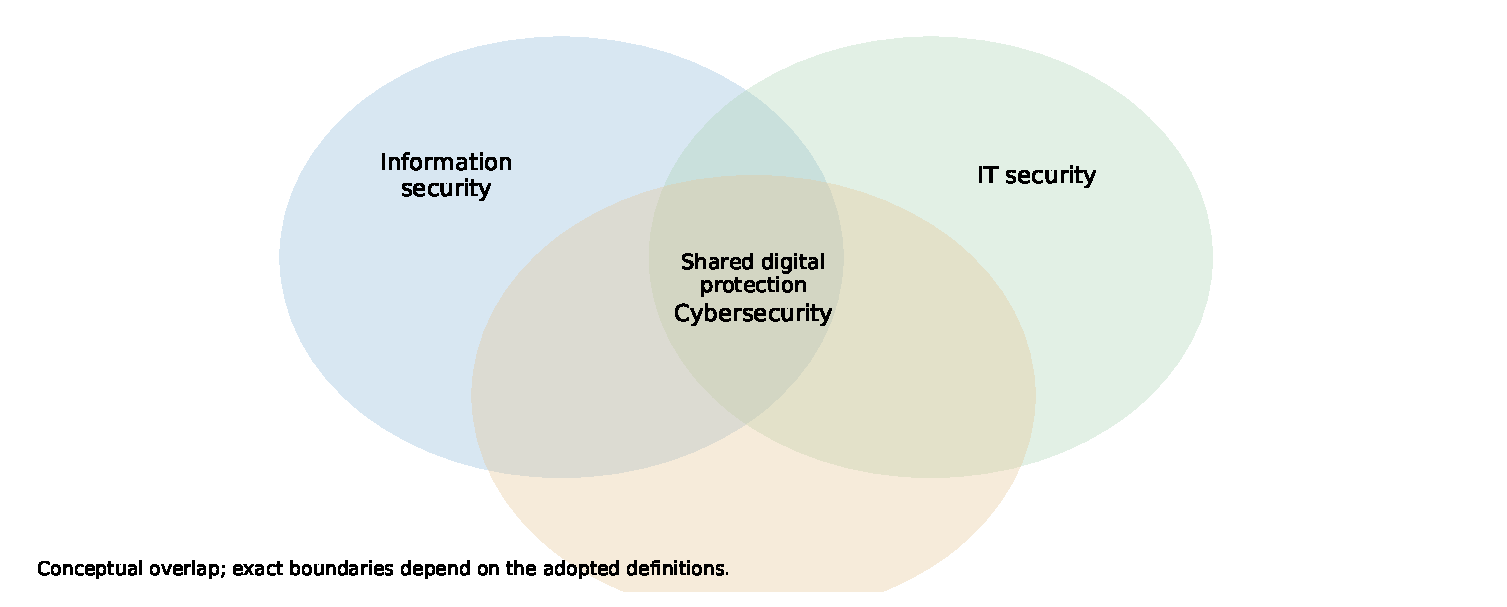
\includegraphics[width=\linewidth,height=.34\textheight,keepaspectratio]{assets/security-scopes.pdf}
\end{center}



The deck's CIA framework applies throughout the overlap. Label this as a conceptual convention,\allowbreak{} since the supplied slides do not define a unique formal set relationship.




\clearpage
\subsection{A046 · 2021–22 · Q2(a)}\label{a046}

\textbf{Classify attacks by the information-security CIA triad · 5 marks}


Original: \href{../../CSE405-Security_Merged.pdf\#page=15}{past-paper PDF p. 15}. Sitting date: 30 October 2023. Printed Section A.


\textbf{Topics:} CIA,\allowbreak{} attacker models and security scope.



\begin{quote}\small

\textbf{Question summary:} Categorize security attacks with respect to confidentiality,\allowbreak{} integrity and availability.



\end{quote}


\Needspace{4\baselineskip}
{\color{ForestGreen}\textbf{Exam tip.} Give a concrete attack for each goal and identify the property it violates.}


Use the \textbf{information-security} CIA triad:



{\small\setlength{\tabcolsep}{3pt}
\begin{longtable}{>{\raggedright\arraybackslash}p{0.19530\linewidth}>{\raggedright\arraybackslash}p{0.35657\linewidth}>{\raggedright\arraybackslash}p{0.40655\linewidth}}
\toprule
\textbf{Goal} & \textbf{Violation} & \textbf{Example} \\
\midrule
\endhead
Confidentiality & Unauthorized disclosure & Eavesdropping on a private conversation or reading a protected file. \\
Integrity & Unauthorized modification or fabrication & Altering a transaction,\allowbreak{} corrupting a file or injecting forged records. \\
Availability & Denial or degradation of timely authorized service & Flooding a server,\allowbreak{} exhausting its connection state or deliberately dropping traffic. \\
\bottomrule
\end{longtable}
}

One attack can violate several goals: malware can steal documents,\allowbreak{} change them and disable access. Classify its particular effects rather than assuming every attack has exactly one category. Authentication helps establish who is acting,\allowbreak{} but \textbf{A here means availability},\allowbreak{} as in Sec A's Introduction PDF p. 2.




\clearpage
\subsection{A066 · 2021–22 · Q8(a)}\label{a066}

\textbf{Delegation through GRANT OPTION and revocation dependencies · 12 marks}


Original: \href{../../CSE405-Security_Merged.pdf\#page=17}{past-paper PDF p. 17}. Sitting date: 30 October 2023. Printed Section B.


\textbf{Topics:} Access matrices,\allowbreak{} ACLs,\allowbreak{} capabilities and RBAC.



\begin{quote}\small

\textbf{Question summary:} Analyze GRANT SELECT ON employees TO Alice WITH GRANT OPTION and revoke access safely when Alice leaves.



\end{quote}

\textbf{Coverage:} related application/\allowbreak{}extension. Access-control delegation is an application of matrices/\allowbreak{}ACLs; DBMS-specific grant/\allowbreak{}revoke syntax is not taught in WebDB-security.



\Needspace{4\baselineskip}
{\color{ForestGreen}\textbf{Exam tip.} Revoke the delegation chain as well as the departing user's own privilege,\allowbreak{} and name the assumed SQL dialect.}


The statement lets Alice read \texttt{employees} and \textbf{delegate SELECT} to other principals. Read-only access to her own session is therefore not the whole authority: she can create additional readers,\allowbreak{} including an account she retains after departure.


On departure,\allowbreak{} remove Alice's direct SELECT and grant option,\allowbreak{} disable her authentication,\allowbreak{} terminate active sessions where needed and audit every grant derived from her authority. In SQL systems supporting dependency-aware cascading revocation,\allowbreak{} the intended form is:



\begin{Verbatim}[breaklines=true,breakanywhere=true,fontsize=\small,frame=single,rulecolor=\color{PanelBorder}]
REVOKE SELECT ON employees FROM Alice CASCADE;
\end{Verbatim}

Exact syntax/\allowbreak{}behavior is DBMS-dependent. PostgreSQL supports cascading dependent grants; MySQL has different privilege/\allowbreak{}revocation semantics and does not accept this generic clause as a portable solution. Inspect the actual grant graph and remove derived rights using the engine's mechanisms. Another independent grant to a recipient may survive revocation of Alice's grant path.


Revocation cannot erase previously copied data. Minimize exposure in advance: avoid unnecessary grant option,\allowbreak{} use managed roles,\allowbreak{} limit sensitive columns/\allowbreak{}rows and review grants.


\href{https://www.postgresql.org/docs/current/sql-revoke.html}{PostgreSQL REVOKE semantics}.




\clearpage
\subsection{A070 · 2020–21 · Q1(b)}\label{a070}

\textbf{Selective packet dropping against a competitor · 12 marks}


Original: \href{../../CSE405-Security_Merged.pdf\#page=18}{past-paper PDF p. 18}. Sitting date: 25 September 2022. Printed Section A.


\textbf{Topics:} CIA,\allowbreak{} attacker models and security scope; DoS/\allowbreak{}DDoS,\allowbreak{} reflection and resource exhaustion.



\begin{quote}\small

\textbf{Question summary:} An ISP deliberately drops 25\% of a competing provider’s VoIP packets traversing its routers. Identify the attack.



\end{quote}


\Needspace{4\baselineskip}
{\color{ForestGreen}\textbf{Exam tip.} Availability includes timely usable service. A 25\% degradation can be a DoS attack without a total outage.}


This is a \textbf{selective denial-of-service/\allowbreak{}degradation attack} by an on-path network operator. It violates availability by making the competitor's voice calls unreliable even if the service is not completely unavailable. The operator abuses a trusted forwarding position; the attacker need not impersonate an endpoint or decrypt the voice content.


Packet loss produces gaps,\allowbreak{} jitter/\allowbreak{}retransmissions where applicable and poor call quality. Encrypting VoIP can protect content and integrity but cannot force a malicious router to forward packets. Detection compares loss/\allowbreak{}quality across paths and traffic classes; mitigation can include independent paths/\allowbreak{}providers and routing around the hostile infrastructure.




\clearpage
\subsection{A071 · 2020–21 · Q1(c)}\label{a071}

\textbf{Why compromise recording matters and which tools support it · 11 marks}


Original: \href{../../CSE405-Security_Merged.pdf\#page=18}{past-paper PDF p. 18}. Sitting date: 25 September 2022. Printed Section A.


\textbf{Topics:} Security principles and scenario analysis; OS trust,\allowbreak{} paging,\allowbreak{} boot and persistent memory images.



\begin{quote}\small

\textbf{Question summary:} Explain the importance of compromise recording and name tools used for it.



\end{quote}


\Needspace{4\baselineskip}
{\color{ForestGreen}\textbf{Exam tip.} A log that nobody checks or an attacker can silently erase is weak compromise recording.}


Prevention can fail,\allowbreak{} so systems need evidence that a violation occurred. Compromise records support detection,\allowbreak{} incident reconstruction,\allowbreak{} identification of affected accounts/\allowbreak{}assets,\allowbreak{} containment and recovery. They can also deter abuse and support accountability.


Examples include OS security/\allowbreak{}event logs,\allowbreak{} authentication and privilege-change auditing,\allowbreak{} application/\allowbreak{}database access logs,\allowbreak{} file-integrity monitoring,\allowbreak{} network flow/\allowbreak{}packet metadata,\allowbreak{} IDS alerts and physical surveillance. A protected central log collector helps preserve evidence when an individual host is compromised.


Record reliable timestamps,\allowbreak{} actor/\allowbreak{}subject,\allowbreak{} action,\allowbreak{} target,\allowbreak{} result and source context. Protect log integrity/\allowbreak{}access,\allowbreak{} monitor collector health,\allowbreak{} retain relevant records and connect alerts to a response process. Logging everything indiscriminately can create privacy,\allowbreak{} storage and analysis problems; select evidence according to the threat model.




\clearpage
\subsection{A072 · 2020–21 · Q2(a)}\label{a072}

\textbf{RBAC diagram,\allowbreak{} benefits and limitations · 12 marks}


Original: \href{../../CSE405-Security_Merged.pdf\#page=18}{past-paper PDF p. 18}. Sitting date: 25 September 2022. Printed Section A.


\textbf{Topics:} Access matrices,\allowbreak{} ACLs,\allowbreak{} capabilities and RBAC.



\begin{quote}\small

\textbf{Question summary:} Define role-based access control with a figure,\allowbreak{} benefits and drawbacks.



\end{quote}


\Needspace{4\baselineskip}
{\color{ForestGreen}\textbf{Exam tip.} Separate user-to-role assignment from role-to-permission assignment in the diagram.}


RBAC associates permissions with organizational \textbf{roles},\allowbreak{} then assigns users to roles. A user's permitted actions come from their active role memberships rather than a separately edited list for every object.



\begin{Verbatim}[breaklines=true,breakanywhere=true,fontsize=\small,frame=single,rulecolor=\color{PanelBorder}]
Alice --+--> Accountant --> read ledger, enter transactions
Bob ----+ 
Carol ------> Auditor ----> read ledger, view audit trail
\end{Verbatim}

Roles can have hierarchies; constraints can enforce separation of duties,\allowbreak{} such as preventing one person from both initiating and approving a payment.


Benefits: simpler onboarding/\allowbreak{}offboarding,\allowbreak{} consistent least-privilege job profiles,\allowbreak{} reusable policy and more understandable audits. Limitations: role explosion when exceptions proliferate,\allowbreak{} stale memberships after job changes,\allowbreak{} conflicts between accumulated roles and difficulty expressing fine-grained context such as time,\allowbreak{} location or a particular patient's care relationship.


A role name alone is not a security control: authenticate the user,\allowbreak{} authorize each operation and review role assignments. Deny unauthorized actions by default.




\clearpage
\subsection{A073 · 2020–21 · Q2(b)}\label{a073}

\textbf{Mismatched boarding-pass and identity checks · 12 marks}


Original: \href{../../CSE405-Security_Merged.pdf\#page=18}{past-paper PDF p. 18}. Sitting date: 25 September 2022. Printed Section A.


\textbf{Topics:} Security principles and scenario analysis; Biometrics,\allowbreak{} authentication factors,\allowbreak{} SIM and RFID.



\begin{quote}\small

\textbf{Question summary:} Explain how online-printable boarding passes permit a no-fly-list bypass in the described airport checks,\allowbreak{} and fix the weakness.



\end{quote}

\textbf{Coverage:} related application/\allowbreak{}extension. An application of complete mediation/\allowbreak{}authentication; the exact airport workflow is in the paper.



\Needspace{4\baselineskip}
{\color{ForestGreen}\textbf{Exam tip.} Show what each checkpoint sees and why two individually plausible documents are not sufficient together.}


The described checks fail to bind \textbf{the same person,\allowbreak{} reservation and boarding pass} across all stages. A listed traveler could book under an unlisted identity. At the ID checkpoint,\allowbreak{} an altered paper pass bearing the traveler's real name might satisfy the local name comparison if the checkpoint does not validate the reservation. At boarding,\allowbreak{} the traveler presents the genuine pass for the unlisted booking if the gate checks the reservation but not the person's ID.


This is an illustrative failure of \textbf{complete mediation and consistent identity binding}. It depends on the precise split checks given in the problem; it is not a statement about every airport's procedures.


Authenticate the pass/\allowbreak{}barcode against the reservation system; bind it to the verified traveler and current screening result; recheck list eligibility and identity at the stages that authorize travel; prevent substitution/\allowbreak{}reuse after checking. A digital signature on the pass protects its fields only if the scanner verifies it and ties it to the person presenting it.



\clearpage
\section{Physical Security}

Primary deck: \href{../slides/Ch02-Physical-Security.pdf}{Ch02-Physical-Security.\allowbreak{}pdf}




\subsection{A044 · 2021–22 · Q1(b)}\label{a044}

\textbf{Biometric requirements,\allowbreak{} recognition pipeline and privacy · 10 marks}


Original: \href{../../CSE405-Security_Merged.pdf\#page=15}{past-paper PDF p. 15}. Sitting date: 30 October 2023. Printed Section A.


\textbf{Topics:} Biometrics,\allowbreak{} authentication factors,\allowbreak{} SIM and RFID.



\begin{quote}\small

\textbf{Question summary:} State biometric identification requirements,\allowbreak{} describe the process,\allowbreak{} and discuss privacy-preserving challenges.



\end{quote}


\Needspace{4\baselineskip}
{\color{ForestGreen}\textbf{Exam tip.} Explain both the matching error tradeoff and the permanence/\allowbreak{}revocation problem.}


A usable biometric should have \textbf{universality} (most people possess it),\allowbreak{} \textbf{distinctiveness},\allowbreak{} \textbf{permanence} and \textbf{collectability}. Practical criteria include accuracy/\allowbreak{}performance,\allowbreak{} user acceptability and resistance to circumvention.



\begin{Verbatim}[breaklines=true,breakanywhere=true,fontsize=\small,frame=single,rulecolor=\color{PanelBorder}]
enrollment: sensor -> quality/liveness checks -> feature extraction -> protected template
recognition: new sample -> features -> compare with template(s) -> threshold decision
\end{Verbatim}

Identification searches a population (\textbf{1:N}); verification checks a claimed identity (\textbf{1:1}). Noise means matching is approximate. Thresholds trade false accepts against false rejects; false enrollment and spoofing are separate risks.


Privacy is difficult because biometrics are persistent identifiers: a stolen fingerprint is hard to revoke,\allowbreak{} templates can enable cross-database linkage,\allowbreak{} and samples may reveal more personal information than necessary. Protect templates with access controls/\allowbreak{}encryption,\allowbreak{} minimize retention,\allowbreak{} separate databases,\allowbreak{} prefer local matching where feasible and use cancellable/\allowbreak{}template-protection methods with careful threat analysis. Plainly hashing a noisy sample does not solve approximate matching. Liveness checks and another factor reduce spoofing risk but do not make a biometric secret.




\clearpage
\subsection{A128 · 2018–19 · Q6(b)}\label{a128}

\textbf{Pin-tumbler cross section · 7 marks}


Original: \href{../../CSE405-Security_Merged.pdf\#page=27}{past-paper PDF p. 27}. Sitting date: 24 October 2019. Printed Section B.


\textbf{Topics:} Pin-tumbler locks and master-key extensions.



\begin{quote}\small

\textbf{Question summary:} Draw a pin-tumbler lock cross section and label its parts.



\end{quote}


\Needspace{4\baselineskip}
{\color{ForestGreen}\textbf{Exam tip.} The pins do not vanish or move sideways; rotation is possible because no solid pin crosses the shear line.}



\begin{center}
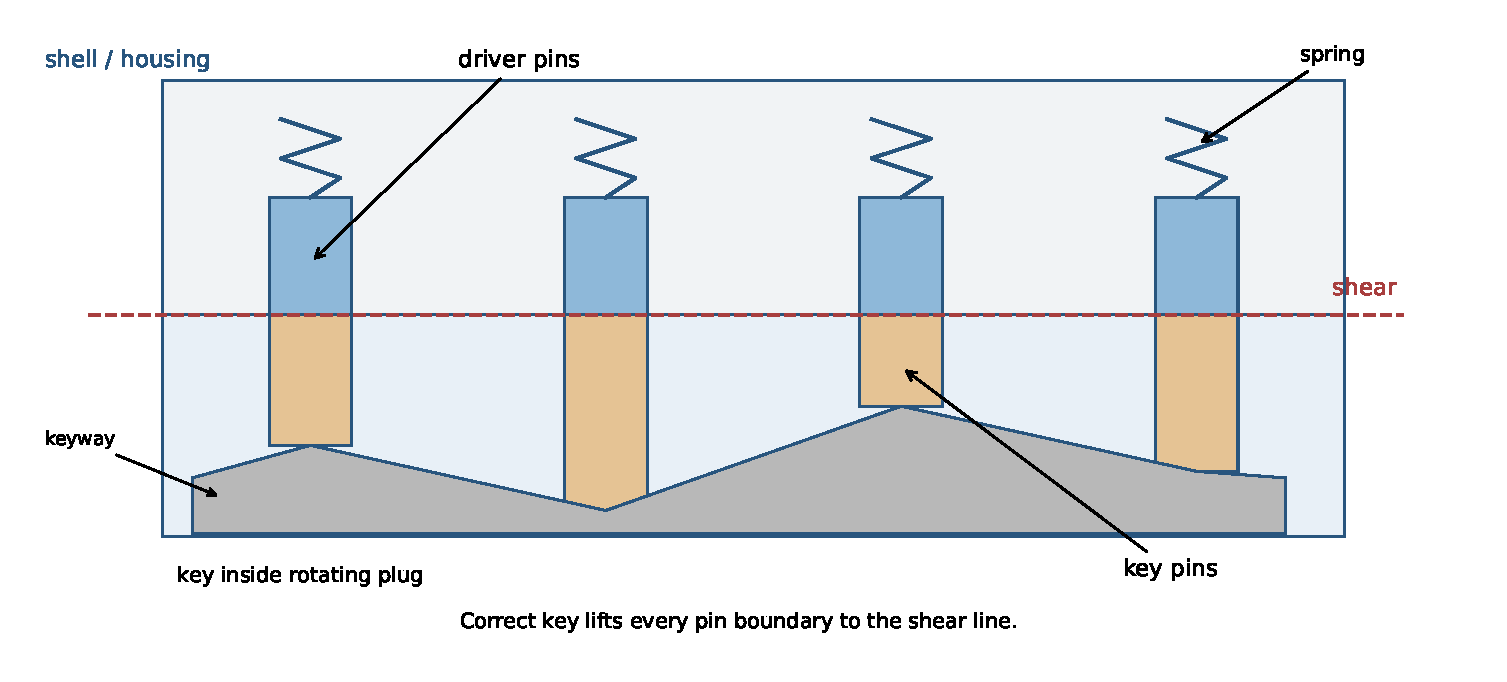
\includegraphics[width=\linewidth,height=.34\textheight,keepaspectratio]{assets/pin-lock.pdf}
\end{center}



The fixed \textbf{housing/\allowbreak{}shell} surrounds a rotatable \textbf{plug} containing the keyway. Each chamber has a spring,\allowbreak{} a driver pin above and a key pin below. With no key or a wrong key,\allowbreak{} a solid pin crosses the shell/\allowbreak{}plug \textbf{shear line},\allowbreak{} blocking rotation.


The correct key lifts each stack until its key-pin/\allowbreak{}driver-pin boundary lies at the shear line. The plug then rotates with the key and actuates the locking mechanism. Label springs,\allowbreak{} driver pins,\allowbreak{} key pins,\allowbreak{} key,\allowbreak{} plug,\allowbreak{} shell and shear line in the diagram.




\clearpage
\subsection{A129 · 2018–19 · Q7(a)}\label{a129}

\textbf{Count additional keys after three master wafers · 3 marks}


Original: \href{../../CSE405-Security_Merged.pdf\#page=27}{past-paper PDF p. 27}. Sitting date: 24 October 2019. Printed Section B.


\textbf{Topics:} Pin-tumbler locks and master-key extensions.



\begin{quote}\small

\textbf{Question summary:} A five-pin lock has driver pins of height 5 and key pins 2,\allowbreak{}4,\allowbreak{}5,\allowbreak{}2,\allowbreak{}6. Add one master wafer in each of three selected chambers. How many additional keys theoretically open it?



\end{quote}

\textbf{Coverage:} related application/\allowbreak{}extension. The deck teaches basic pin-tumbler operation; master-wafer combinatorics is an extension.



\Needspace{4\baselineskip}
{\color{ForestGreen}\textbf{Exam tip.} Distinguish eight total keys from seven additional keys.}


Assume the three selected chambers each gain \textbf{two distinct usable shear boundaries},\allowbreak{} and the resulting cut choices are independent and physically valid. Each contributes two possible cut heights; unchanged chambers contribute one.



\[
\text{total theoretical key profiles}=2^3=8.
\]

The original working key is one profile,\allowbreak{} so the number of \textbf{additional} theoretical keys is



\[
8-1=\boxed{7}.
\]

Driver-pin height and the original key-pin values are not needed for this count. Real bitting restrictions,\allowbreak{} wafer dimensions or coincident/\allowbreak{}unusable boundaries can reduce it; the question says theoretically.




\clearpage
\subsection{A130 · 2018–19 · Q7(b)}\label{a130}

\textbf{Construct a lock accepting both stated keys · 12 marks}


Original: \href{../../CSE405-Security_Merged.pdf\#page=27}{past-paper PDF p. 27}. Sitting date: 24 October 2019. Printed Section B.


\textbf{Topics:} Pin-tumbler locks and master-key extensions.



\begin{quote}\small

\textbf{Question summary:} Given L1 key-pin heights (2,\allowbreak{}4,\allowbreak{}5,\allowbreak{}2,\allowbreak{}6) and L2 (4,\allowbreak{}2,\allowbreak{}5,\allowbreak{}5,\allowbreak{}6),\allowbreak{} driver heights 5,\allowbreak{} design L3 with master wafers so both keys work,\allowbreak{} and show K1 opening it.



\end{quote}

\textbf{Coverage:} related application/\allowbreak{}extension. Master-key construction extends the basic lock slides; the geometric interpretation is stated explicitly.



\Needspace{4\baselineskip}
{\color{ForestGreen}\textbf{Exam tip.} Use a shorter bottom pin plus the difference wafer; two original pin lengths placed in series do not create the intended boundaries.}


Use a common key datum/\allowbreak{}shear height \(H\) and interpret the supplied numbers as the key-pin lengths required by the two key profiles. In each chamber take the \textbf{smaller key pin} and a wafer equal to the absolute difference:



{\small\setlength{\tabcolsep}{3pt}
\begin{longtable}{>{\raggedright\arraybackslash}p{0.14661\linewidth}>{\raggedright\arraybackslash}p{0.13573\linewidth}>{\raggedright\arraybackslash}p{0.13573\linewidth}>{\raggedright\arraybackslash}p{0.17523\linewidth}>{\raggedright\arraybackslash}p{0.19196\linewidth}>{\raggedright\arraybackslash}p{0.13573\linewidth}}
\toprule
\textbf{Chamber} & \textbf{L1 pin} & \textbf{L2 pin} & \textbf{L3 key pin} & \textbf{Master wafer} & \textbf{Driver} \\
\midrule
\endhead
1 & 2 & 4 & 2 & 2 & 5 \\
2 & 4 & 2 & 2 & 2 & 5 \\
3 & 5 & 5 & 5 & none & 5 \\
4 & 2 & 5 & 2 & 3 & 5 \\
5 & 6 & 6 & 6 & none & 5 \\
\bottomrule
\end{longtable}
}

For a concrete sketch choose \(H=10\). K1 lifts the stacks by \((8,6,5,8,4)\) units,\allowbreak{} since lift equals \(H\) minus its corresponding original key-pin length. In chamber 1 the top of the 2-unit key pin is at \(H\) (wafer above); in chamber 2 the top of key pin plus wafer is at \(H\); chambers 3/\allowbreak{}5 have their ordinary boundary at \(H\); chamber 4 uses the top of its 2-unit pin with wafer above. Thus no solid pin crosses the shear line.


K2 uses lifts \((6,8,5,5,4)\),\allowbreak{} selecting the alternative boundary in chambers 1,\allowbreak{}2,\allowbreak{}4. Keep adequate spring/\allowbreak{}chamber clearance for the chosen dimensions.



\begin{center}
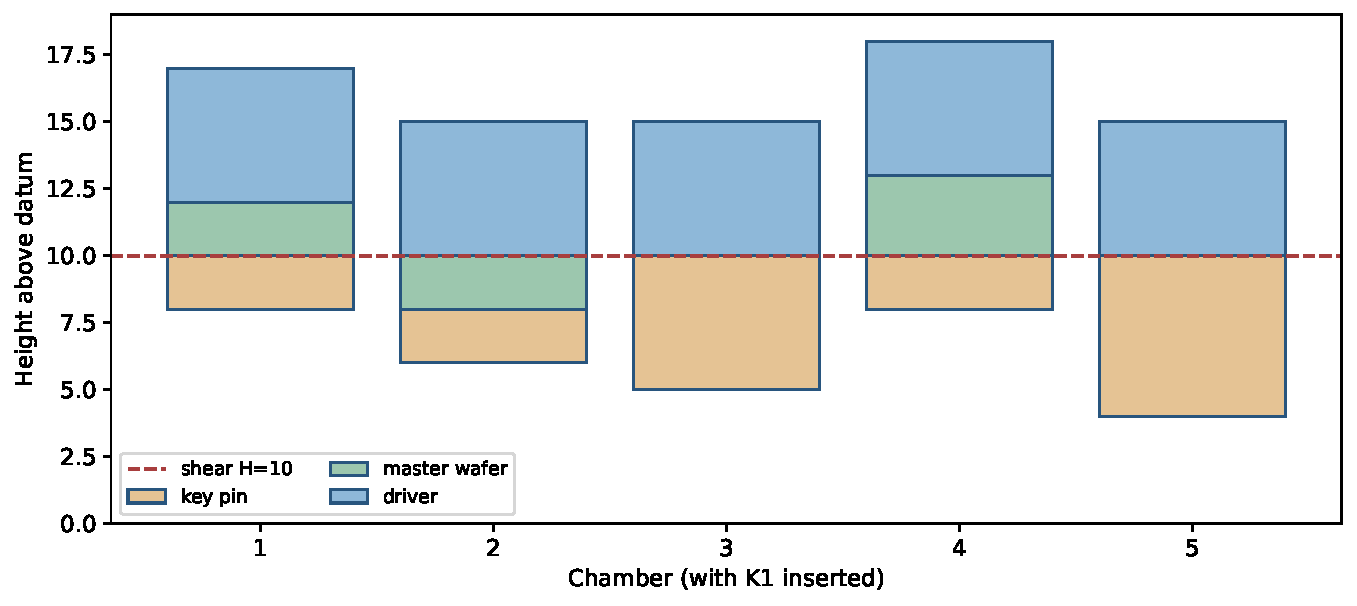
\includegraphics[width=\linewidth,height=.34\textheight,keepaspectratio]{assets/master-lock.pdf}
\end{center}



Three independently mastered chambers theoretically also admit six unintended mixed profiles besides the two named keys: \(2^3-2=6\).




\clearpage
\subsection{A131 · 2018–19 · Q8(a)}\label{a131}

\textbf{Good biometric criteria · 6 marks}


Original: \href{../../CSE405-Security_Merged.pdf\#page=28}{past-paper PDF p. 28}. Sitting date: 24 October 2019. Printed Section B.


\textbf{Topics:} Biometrics,\allowbreak{} authentication factors,\allowbreak{} SIM and RFID.



\begin{quote}\small

\textbf{Question summary:} Name essential and desirable characteristics of biometric authentication.



\end{quote}


\Needspace{4\baselineskip}
{\color{ForestGreen}\textbf{Exam tip.} Give a short explanation of each property; “secure and fast” is too vague.}


The usual core criteria are \textbf{universality},\allowbreak{} \textbf{distinctiveness/\allowbreak{}uniqueness},\allowbreak{} \textbf{permanence} and \textbf{collectability}. A useful implementation also needs good \textbf{performance} (speed,\allowbreak{} accuracy and robustness),\allowbreak{} \textbf{acceptability} to users and resistance to \textbf{circumvention} such as spoofed samples.


In practice these are degrees rather than absolutes: some people lack a measurable feature,\allowbreak{} samples change with age/\allowbreak{}injury,\allowbreak{} and environmental noise affects capture. Provide alternatives and evaluate false-accept/\allowbreak{}false-reject rates rather than promising perfect identity recognition.




\clearpage
\subsection{A132 · 2018–19 · Q8(b)}\label{a132}

\textbf{Faraday cage and OS impersonation-token short notes · 9 printed marks (mixed question)}


Original: \href{../../CSE405-Security_Merged.pdf\#page=28}{past-paper PDF p. 28}. Sitting date: 24 October 2019. Printed Section B.


\textbf{Topics:} Faraday shielding and physical information leakage; OS trust,\allowbreak{} paging,\allowbreak{} boot and persistent memory images.



\begin{quote}\small

\textbf{Question summary:} From the printed “any three” short notes,\allowbreak{} cover the Sec A options: (i) Faraday cage and (iii) impersonation token.



\end{quote}

\textbf{Sec A scope:} Covers only options (i) Faraday cage and (iii) OS impersonation token,\allowbreak{} 3 marks each. Options (ii) blind SQL injection and (iv) homograph attack remain in Sec B. The printed 9 marks require any three choices.


\textbf{Coverage:} related application/\allowbreak{}extension. The printed subquestion is 9 marks for any three choices. This guide covers only two Sec A choices (3 marks each); it is not a full 9-mark answer. OS impersonation-token mechanics extend the supplied privilege material.



\Needspace{4\baselineskip}
{\color{ForestGreen}\textbf{Exam tip.} Keep shielding under physical security and impersonation under OS identity/\allowbreak{}privilege. The printed question's remaining two options belong to Sec B and are excluded from this answer.}


\textbf{(i) Faraday cage.} A conductive enclosure attenuates electromagnetic coupling between its interior and exterior. Charge redistribution and induced currents help shield against external fields and reduce information leakage from electronic emanations. In computer security,\allowbreak{} shielding can protect equipment or reduce unintended radio emissions. Its effectiveness depends on frequency,\allowbreak{} material,\allowbreak{} seams,\allowbreak{} openings and construction; it does not guarantee perfect isolation at every frequency or block unrelated acoustic leakage.


\textbf{(iii) Impersonation token.} In an operating-system security context,\allowbreak{} a token represents a principal's security context,\allowbreak{} such as identity,\allowbreak{} groups and privileges. A server thread can temporarily impersonate a client so that access checks use the client's rights rather than the server's broader authority. This supports least privilege when the token and permitted impersonation level are properly checked. Token theft or excessive impersonation rights can permit unauthorized access. Limit the scope,\allowbreak{} protect token handles and reliably restore the original context after the operation.


\href{https://learn.microsoft.com/en-us/windows/win32/secauthz/access-tokens}{Microsoft access-token documentation} describes these identity and privilege contexts.


The OS-token explanation extends the supplied process-privilege material. It is distinct from a web session cookie and is not a SQL-injection mechanism.




\clearpage
\subsection{A134 · 2018–19 · Q9(b)}\label{a134}

\textbf{Expand ICCID,\allowbreak{} IMSI and ASLR · 3 marks}


Original: \href{../../CSE405-Security_Merged.pdf\#page=28}{past-paper PDF p. 28}. Sitting date: 24 October 2019. Printed Section B.


\textbf{Topics:} Biometrics,\allowbreak{} authentication factors,\allowbreak{} SIM and RFID; StackGuard,\allowbreak{} ASLR and memory-corruption defenses.



\begin{quote}\small

\textbf{Question summary:} Write the full forms of ICCID,\allowbreak{} IMSI and ASLR.



\end{quote}

\textbf{Coverage:} related application/\allowbreak{}extension. SIM identifiers are in the physical deck/\allowbreak{}notes; ASLR is a memory-defense extension.



\Needspace{4\baselineskip}
{\color{ForestGreen}\textbf{Exam tip.} Write “Identity” for IMSI and “Randomization” for ASLR.}



\begin{itemize}

\item \textbf{ICCID:} Integrated Circuit Card Identifier.

\item \textbf{IMSI:} International Mobile Subscriber Identity.

\item \textbf{ASLR:} Address Space Layout Randomization.

\end{itemize}

ICCID identifies the card/\allowbreak{}profile; IMSI identifies the mobile subscription. Neither should be confused with a phone number. ASLR randomizes memory locations to make address prediction harder; it does not correct an unsafe memory access.



\clearpage
\section{Operating Systems Security}

Primary deck: \href{../slides/Ch03-OS-Security.pdf}{Ch03-OS-Security.\allowbreak{}pdf}




\subsection{A053 · 2021–22 · Q4(a)}\label{a053}

\textbf{Secrets persisted in swap/\allowbreak{}hibernation · 5 marks}


Original: \href{../../CSE405-Security_Merged.pdf\#page=16}{past-paper PDF p. 16}. Sitting date: 30 October 2023. Printed Section A.


\textbf{Topics:} OS trust,\allowbreak{} paging,\allowbreak{} boot and persistent memory images.



\begin{quote}\small

\textbf{Question summary:} Explain how virtual memory or a swap partition can be an attacker target.



\end{quote}


\Needspace{4\baselineskip}
{\color{ForestGreen}\textbf{Exam tip.} Connect the RAM secret to its disk copy; “virtual memory is fake memory” is not an explanation.}


Paging can write memory pages to disk; hibernation writes a much larger memory snapshot. Passwords,\allowbreak{} keys,\allowbreak{} documents and session tokens that were temporarily present in RAM can therefore remain in swap/\allowbreak{}hibernation storage after an application exits or the screen locks.


An attacker with physical disk access,\allowbreak{} an alternate boot path or sufficient privileges may extract those remnants,\allowbreak{} bypassing the original OS's access checks. Virtual memory itself is not a vulnerability: the exposure is sensitive state persisted without suitable protection.


Use disk/\allowbreak{}swap encryption with appropriate key handling,\allowbreak{} protect boot and physical access,\allowbreak{} restrict dump/\allowbreak{}image files and minimize secret lifetime. An encrypted disk whose key is accessible to an attacker in a live unlocked system has a different threat model.




\clearpage
\subsection{A074 · 2020–21 · Q2(c)}\label{a074}

\textbf{Forensic preservation: master and working images,\allowbreak{} custody · 11 marks}


Original: \href{../../CSE405-Security_Merged.pdf\#page=18}{past-paper PDF p. 18}. Sitting date: 25 September 2022. Printed Section A.


\textbf{Topics:} OS trust,\allowbreak{} paging,\allowbreak{} boot and persistent memory images.



\begin{quote}\small

\textbf{Question summary:} Why make two copies of digital evidence? State precautions and how to maintain chain of custody.



\end{quote}

\textbf{Coverage:} related application/\allowbreak{}extension. OS/\allowbreak{}hibernation notes mention forensic investigation; full acquisition and custody procedures are supplementary.



\Needspace{4\baselineskip}
{\color{ForestGreen}\textbf{Exam tip.} Explain what each copy is for and how you establish that it faithfully represents the acquired evidence.}


Keep one verified \textbf{preservation/\allowbreak{}master image} and use a separate \textbf{working copy} for examination. Analysis can alter metadata,\allowbreak{} recovery state or software behavior; a preserved baseline allows repeatable checking. Preserve the original device as well,\allowbreak{} when applicable. Merely possessing two unverified copies proves nothing.


Acquire a suitable bit-stream image using validated tools and a write blocker where appropriate. Record device identifiers,\allowbreak{} acquisition time,\allowbreak{} tool/\allowbreak{}version,\allowbreak{} operator and relevant system state. Hash the acquired image with a suitable cryptographic hash and verify copied images against it. Decide separately how to capture volatile evidence before power changes; imaging a live system may itself change data and needs documented handling.


Maintain a custody record for every transfer: evidence ID,\allowbreak{} who released/\allowbreak{}received it,\allowbreak{} timestamps,\allowbreak{} purpose,\allowbreak{} storage/\allowbreak{}location and integrity checks. Store originals/\allowbreak{}master images with restricted access and tamper-evident handling. A hash establishes consistency,\allowbreak{} while custody documentation establishes the handling history; neither substitutes for the other.


\href{https://nvlpubs.nist.gov/nistpubs/legacy/sp/nistspecialpublication800-86.pdf}{Technical reference: NIST SP 800-86}.




\clearpage
\subsection{A075 · 2020–21 · Q3(a)}\label{a075}

\textbf{Why preserve memory-region boundaries? · 12 marks}


Original: \href{../../CSE405-Security_Merged.pdf\#page=18}{past-paper PDF p. 18}. Sitting date: 25 September 2022. Printed Section A.


\textbf{Topics:} OS trust,\allowbreak{} paging,\allowbreak{} boot and persistent memory images; Stack/\allowbreak{}heap corruption and buffer-overflow payload reasoning.



\begin{quote}\small

\textbf{Question summary:} Explain the risks of mixing heap and stack storage and give an example manipulation.



\end{quote}


\Needspace{4\baselineskip}
{\color{ForestGreen}\textbf{Exam tip.} Distinguish address-space sharing from unsafe overlap or lack of bounds enforcement.}


Stack storage follows call/\allowbreak{}return lifetimes; heap allocations have explicit allocator-managed lifetimes. Both usually occupy one process's \textbf{virtual address space} already. The security goal is valid bounds,\allowbreak{} lifetimes and suitable protections—not a false claim that separate labeled regions prevent all overflow.


If an unchecked heap allocation/\allowbreak{}overflow can reach live stack control data,\allowbreak{} an attacker can corrupt local state,\allowbreak{} saved frame pointers or return addresses. Conversely,\allowbreak{} an unbounded stack allocation can collide with heap mappings or other regions if guards/\allowbreak{}limits are absent. For example,\allowbreak{} copying an oversized request into a heap buffer adjacent to a control structure can overwrite a callback pointer; if storage is mixed with a stack frame,\allowbreak{} the analogous overwrite may replace the saved return address.


Region separation and guard pages reduce accidental collisions and help enforce stack/\allowbreak{}heap limits. They are not complete isolation within the process: an arbitrary write can still target either region. Use bounds/\allowbreak{}lifetime-safe code,\allowbreak{} guarded mappings,\allowbreak{} allocation checks and control-flow defenses.



\clearpage
\section{Buffer Overflow}

Primary deck: \href{../slides/Ch03-BufferOverflow.pdf}{Ch03-BufferOverflow.\allowbreak{}pdf}




\subsection{A001 · 2023–24 · Q1(a)}\label{a001}

\textbf{Trace the actual unsafe copies and construct a conditional control-flow payload · 10 marks}


Original: \href{../../CSE405-Security_Merged.pdf\#page=1}{past-paper PDF p. 1}. Sitting date: 06 September 2025. Printed Section A.


\textbf{Topics:} Stack/\allowbreak{}heap corruption and buffer-overflow payload reasoning.



\begin{quote}\small

\textbf{Question summary:} For the printed 32-bit little-endian C program,\allowbreak{} decide whether hack() can be invoked and give symbolic-address payload pseudocode. All defenses are disabled; main reads 300 bytes into str[30]; overflow\_in\_action has buffer[300],\allowbreak{} two heap pointers,\allowbreak{} strcpy calls and an indirect callback.



\end{quote}

\textbf{Coverage:} related application/\allowbreak{}extension. The source does not fix frame offsets or heap allocator layout. A conditional symbolic payload is justified; an unconditional offset is not.



\Needspace{4\baselineskip}
{\color{ForestGreen}\textbf{Exam tip.} Mark the destination and bound for every write. A stack overflow and a heap overflow have different reachable targets.}


\textbf{Find all three writes before choosing an attack.} \texttt{fread(str,\allowbreak{}1,\allowbreak{}300,\allowbreak{}...)} already overflows main's 30-byte stack array. It does not append a NUL. \texttt{strcpy(buffer,\allowbreak{}str)} may also exceed 300 bytes if no earlier terminator exists. Finally,\allowbreak{} \texttt{strcpy(data->name,\allowbreak{}str)} overruns the 30-byte heap allocation for sufficiently long strings.


A robust exam answer uses the first overflow to replace \textbf{main's saved return address},\allowbreak{} provided execution survives the intervening copies/\allowbreak{}callback and returns normally. Define \(S\) as the address of \texttt{str[0]},\allowbreak{} \(R\) as the address of main's saved return word,\allowbreak{} \(H\) as the address of \texttt{hack},\allowbreak{} and \(d=R-S\). Derive \(d\) from the actual frame; declaration order does not specify padding/\allowbreak{}alignment.



\begin{Verbatim}[breaklines=true,breakanywhere=true,fontsize=\small,frame=single,rulecolor=\color{PanelBorder}]
from struct import pack
# S, R, H come from the particular exam/debugger stack layout.
d = R - S
assert 30 <= d and d + 5 <= 300
payload = b'A' * d + pack('<I', H) + b'\0'
\end{Verbatim}

The terminating zero bounds subsequent copies \textbf{only if} the packed address contains no earlier zero; it does not undo their memory corruption. This payload establishes the intended overwritten return word,\allowbreak{} but success is conditional on heap layout,\allowbreak{} valid pointer variables,\allowbreak{} allocation metadata and successful return from \texttt{overflow\_in\_action}. A chain may need to preserve intervening words. If \texttt{hack} returns,\allowbreak{} a valid continuation is also needed.


\textbf{Do not invent a heap adjacency guarantee.} \texttt{ptr} is allocated before \texttt{data}; an ordinary forward overflow from \texttt{data->name} does not necessarily overwrite the earlier callback allocation. Also \texttt{ptr->fp=\allowbreak{}random\_print} is assigned after the stack copy. The printed C plus “all defenses disabled” does not determine a universal byte-exact successful payload. State the layout/\allowbreak{}survival assumptions instead of claiming that 30 heap bytes automatically reach \texttt{fp}.


\textbf{Fix:} read at most \texttt{sizeof str-1} bytes,\allowbreak{} terminate explicitly,\allowbreak{} validate lengths before both copies,\allowbreak{} and eliminate unnecessary mutable callback/\allowbreak{}heap state.




\clearpage
\subsection{A005 · 2023–24 · Q2(b)}\label{a005}

\textbf{Leaked stack address and one-byte saved-frame-pointer overwrite · 10 marks}


Original: \href{../../CSE405-Security_Merged.pdf\#page=3}{past-paper PDF p. 3}. Sitting date: 06 September 2025. Printed Section A.


\textbf{Topics:} Stack/\allowbreak{}heap corruption and buffer-overflow payload reasoning; StackGuard,\allowbreak{} ASLR and memory-corruption defenses.



\begin{quote}\small

\textbf{Question summary:} 32-bit x86 with ASLR: main prints simple[32] address and reads with fgets(simple,\allowbreak{}32). hack copies nine input bytes backward into buf[8]. Construct inputs for a 31-byte shellcode,\allowbreak{} identifying necessary stack-layout assumptions.



\end{quote}

\textbf{Coverage:} related application/\allowbreak{}extension. Compiler local ordering,\allowbreak{} padding and the location of a surviving fake frame are not specified,\allowbreak{} so the intended off-by-one exploit is conditional.



\Needspace{4\baselineskip}
{\color{ForestGreen}\textbf{Exam tip.} A leaked address bypasses secrecy,\allowbreak{} not bounds checks or frame-layout constraints. Show both the one-byte overwrite and the later pivot.}


The first input can put the \textbf{31-byte shellcode} in \texttt{simple}; \texttt{fgets(...,\allowbreak{}32,\allowbreak{}...)} reads at most 31 bytes and appends NUL. The printed address \(S\) reveals its location despite ASLR. Shellcode bytes must be suitable for this input path (in particular,\allowbreak{} avoid an early newline). Executable stack is assumed because other defenses are disabled.


The second read fills \texttt{input[9]} exactly. The loop's first write is \texttt{buf[8]=\allowbreak{}input[8]},\allowbreak{} one byte beyond \texttt{buf}. The intended exploit is an \textbf{off-by-one saved-EBP overwrite}. This requires \texttt{buf+8} to be the low byte of saved EBP; compiler padding or a different local ordering defeats that premise. The source alone does not establish this layout.


With a \texttt{leave; ret} epilogue,\allowbreak{} corrupting hack's saved EBP changes the EBP restored in main. When main later executes \texttt{leave},\allowbreak{} it pivots ESP to a chosen address \(F\). The word at \(F\) is treated as saved EBP and the word at \(F+4\) as the return address. Place \(S\) at \(F+4\) and arrange a usable continuation. Because only one byte is changed,\allowbreak{} \(F\) must share the original saved frame pointer's upper 24 bits; a low-byte wrap cannot change the other bytes.


One possible \textbf{conditional layout} puts a fake two-word frame in the eight controlled bytes of \texttt{buf},\allowbreak{} sets the ninth byte to the low byte of its address,\allowbreak{} and returns into \texttt{simple}. It additionally requires that this memory survive main's epilogue and that saved EBP has the required upper bytes. Alternatively place a fake frame in another controlled area satisfying the same constraints. A 31-byte shellcode already consumes almost all of \texttt{simple}; do not silently also assume eight extra writable frame bytes fit there.


Under that intended layout,\allowbreak{} define \(F\) as the address of \texttt{buf[0]} and \(M\) as main's original frame pointer. The second input has the concrete symbolic form:



\begin{Verbatim}[breaklines=true,breakanywhere=true,fontsize=\small,frame=single,rulecolor=\color{PanelBorder}]
from struct import pack
assert (F & 0xffffff00) == (M & 0xffffff00)
second_input = pack('<I', 0x41414141) + pack('<I', S) + bytes([F & 0xff])
# 8 bytes form the fake frame in buf; byte 9 alters saved EBP.
\end{Verbatim}

The first input is the stipulated 31-byte shellcode itself; \texttt{fgets} supplies its terminating NUL. The fake frame's first word becomes EBP after main's \texttt{leave},\allowbreak{} while its second word transfers to \(S\). A shellcode that does not return avoids needing a valid later stack continuation. Without the assumed adjacency/\allowbreak{}address relation this byte sequence is not guaranteed to work.




\clearpage
\subsection{A083 · 2020–21 · Q5(c)}\label{a083}

\textbf{Four defenses against return-to-libc · 10 marks}


Original: \href{../../CSE405-Security_Merged.pdf\#page=19}{past-paper PDF p. 19}. Sitting date: 25 September 2022. Printed Section B.


\textbf{Topics:} Return-to-libc and calling conventions; StackGuard,\allowbreak{} ASLR and memory-corruption defenses.



\begin{quote}\small

\textbf{Question summary:} Briefly explain four countermeasures against return-to-libc attacks.



\end{quote}

\textbf{Coverage:} related application/\allowbreak{}extension. Buffer-overflow basics are taught; code reuse and several defense mechanisms require supplementary material.



\Needspace{4\baselineskip}
{\color{ForestGreen}\textbf{Exam tip.} State what each defense interrupts and one relevant limitation; do not count “NX” as if it prevents code reuse by itself.}



\begin{enumerate}

\item \textbf{Remove the memory-corruption primitive:} bounded operations,\allowbreak{} correct allocation/\allowbreak{}lifetime checks and memory-safe implementation prevent the overwrite used to redirect control.

\item \textbf{Stack canaries:} verify a protected value before returning to detect many contiguous overwrites of saved control data. Leaks and noncontiguous writes can bypass this protection.

\item \textbf{ASLR with PIE and randomized libraries:} make target code/\allowbreak{}data addresses hard to predict. Information leaks and weak entropy reduce its effectiveness.

\item \textbf{Control-flow/\allowbreak{}return protection:} a protected shadow stack checks return addresses; suitable CFI constrains indirect transfers. These directly limit forged return/\allowbreak{}call chains,\allowbreak{} subject to the mechanism's coverage.

\end{enumerate}

A non-executable stack alone is \textbf{not} a sufficient return-to-libc defense: the attack reuses existing executable code. W\textasciicircum{}X/\allowbreak{}NX still reduces code-injection options and belongs in layered protection.




\clearpage
\subsection{A085 · 2020–21 · Q6(c)}\label{a085}

\textbf{Place system arguments using 32-bit cdecl · 10 marks}


Original: \href{../../CSE405-Security_Merged.pdf\#page=20}{past-paper PDF p. 20}. Sitting date: 25 September 2022. Printed Section B.


\textbf{Topics:} Return-to-libc and calling conventions.



\begin{quote}\small

\textbf{Question summary:} Using diagrams,\allowbreak{} determine placement of the system() argument in a return-to-libc attack.



\end{quote}

\textbf{Coverage:} related application/\allowbreak{}extension. The supplied C/\allowbreak{}stack material is background; the cdecl libc-chain layout is an extension.



\Needspace{4\baselineskip}
{\color{ForestGreen}\textbf{Exam tip.} Simulate ESP after each \texttt{ret}; that removes the common off-by-four mistake.}


Assume the paper's conventional \textbf{32-bit x86 cdecl} frame and a vulnerable function whose saved return address can be overwritten. Let \(R\) denote that saved return slot,\allowbreak{} \(S\) the address of \texttt{system},\allowbreak{} \(E\) a usable continuation such as \texttt{exit},\allowbreak{} and \(B\) a valid pointer to the NUL-terminated command string in this toy layout.



\begin{Verbatim}[breaklines=true,breakanywhere=true,fontsize=\small,frame=single,rulecolor=\color{PanelBorder}]
higher addresses
R+8   B       first argument to system
R+4   E       system's apparent return address
R     S       vulnerable function's overwritten return address
... padding/local buffer ...
lower addresses
\end{Verbatim}

When the vulnerable function executes \texttt{ret},\allowbreak{} it loads EIP from \(R\) and ESP becomes \(R+4\). On entry,\allowbreak{} \texttt{system} expects its return address at \texttt{[ESP]} and its first argument at \texttt{[ESP+4]},\allowbreak{} so the argument belongs at \textbf{R+8},\allowbreak{} not immediately after the overwritten return word.


If \texttt{system} returns,\allowbreak{} a safe continuation needs its own correctly arranged arguments/\allowbreak{}frame; simply writing an \texttt{exit} address does not guarantee a clean exit status argument. Addresses,\allowbreak{} offset to \(R\),\allowbreak{} input NUL constraints,\allowbreak{} ASLR and canary state must be established for the exact program.



\begin{center}
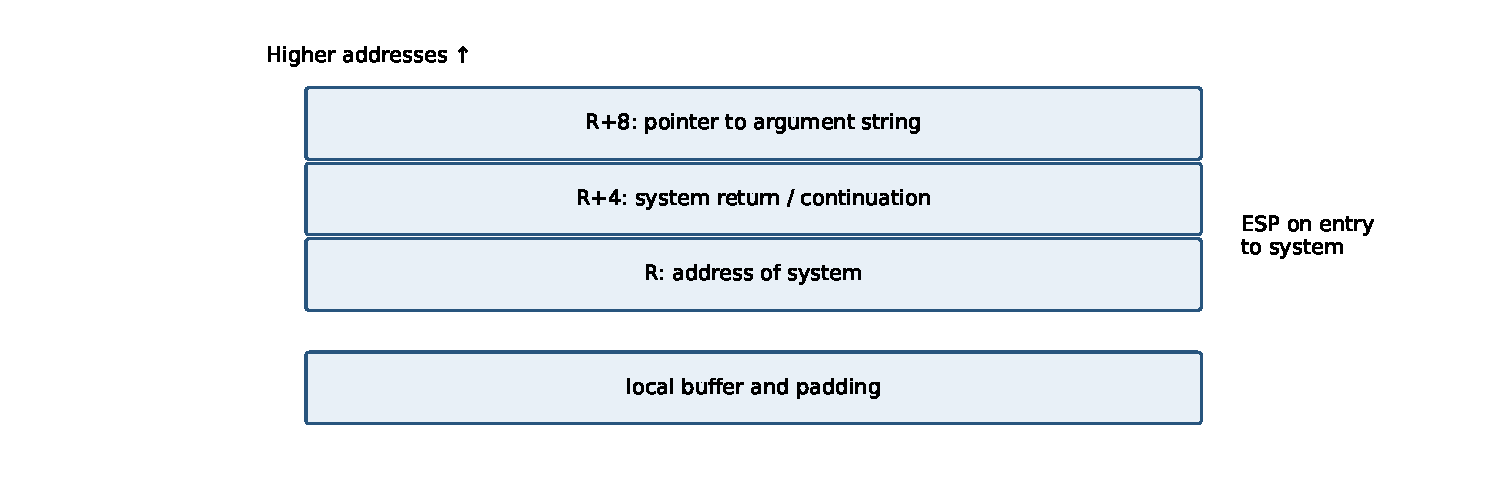
\includegraphics[width=\linewidth,height=.34\textheight,keepaspectratio]{assets/retlibc-stack.pdf}
\end{center}



This arrangement does not carry over unchanged to x86-64 ABIs,\allowbreak{} which generally pass initial arguments in registers.




\clearpage
\subsection{A086 · 2020–21 · Q7(c)}\label{a086}

\textbf{StackGuard check and scope · 10 marks}


Original: \href{../../CSE405-Security_Merged.pdf\#page=20}{past-paper PDF p. 20}. Sitting date: 25 September 2022. Printed Section B.


\textbf{Topics:} StackGuard,\allowbreak{} ASLR and memory-corruption defenses.



\begin{quote}\small

\textbf{Question summary:} Define StackGuard and explain with a diagram how it counters buffer overflow.



\end{quote}


\Needspace{4\baselineskip}
{\color{ForestGreen}\textbf{Exam tip.} Put the check before control transfer and state which overwrite path crosses the canary.}


StackGuard is a compiler-inserted stack-canary defense. A protected word is placed between vulnerable stack storage and saved control data in a function frame. Before returning,\allowbreak{} generated code checks that the canary still equals its expected value; a mismatch aborts rather than using a corrupted return address.



\begin{Verbatim}[breaklines=true,breakanywhere=true,fontsize=\small,frame=single,rulecolor=\color{PanelBorder}]
higher addresses: caller state / return address
                  saved frame pointer
                  CANARY  <-- checked before return
                  local arrays / other locals
lower addresses
\end{Verbatim}

A conventional sequential overflow from a local buffer toward the return address must cross the canary. Random canaries make an unseen correct replacement difficult; some historical schemes use terminator values to obstruct string copying. Exact frame ordering depends on implementation.


This \textbf{detects some corruption},\allowbreak{} not the unsafe write itself. A canary leak,\allowbreak{} an overwrite that skips the canary,\allowbreak{} corruption of non-control data or a heap attack may avoid the check. A process may also be harmed before reaching its epilogue. Combine it with bounds-safe code,\allowbreak{} ASLR,\allowbreak{} NX and control-flow protection.




\clearpage
\subsection{A087 · 2020–21 · Q8(a)}\label{a087}

\textbf{Audit scanf,\allowbreak{} privileged file opening and a name-based access race · 15 marks}


Original: \href{../../CSE405-Security_Merged.pdf\#page=20}{past-paper PDF p. 20}. Sitting date: 25 September 2022. Printed Section B.


\textbf{Topics:} Stack/\allowbreak{}heap corruption and buffer-overflow payload reasoning; Unix permissions,\allowbreak{} setuid and filesystem access; Security principles and scenario analysis.



\begin{quote}\small

\textbf{Question summary:} Analyze attacks on the printed C program (code on p. 21): scanf into buffer[60],\allowbreak{} fopen(fn,\allowbreak{}"a+"),\allowbreak{} access(fn,\allowbreak{}W\_OK),\allowbreak{} fwrite; state environmental assumptions.



\end{quote}

\textbf{Coverage:} related application/\allowbreak{}extension. Unsafe C,\allowbreak{} Unix privileges and complete-mediation principles support the answer; the exact race analysis is an application.



\Needspace{4\baselineskip}
{\color{ForestGreen}\textbf{Exam tip.} Trace object identity through the descriptor. This example is an open-then-check race,\allowbreak{} not the usual check-then-open ordering.}


\textbf{Unbounded input:} \texttt{scanf("\%s",\allowbreak{}buffer)} has no width,\allowbreak{} so an input exceeding the 60-byte array (including its terminator) can corrupt neighboring locals or saved control state. A specific control-flow attack depends on frame layout,\allowbreak{} address knowledge,\allowbreak{} protections and process privileges. Use a bounded read,\allowbreak{} check its result and handle long input deliberately.


\textbf{Privilege/\allowbreak{}identity mismatch:} if this is a setuid program,\allowbreak{} \texttt{fopen} uses effective-identity permissions,\allowbreak{} whereas \texttt{access} ordinarily checks the real identity. Opening before the authorization decision may already create a file or otherwise have effects; the program should not acquire unauthorized capabilities and then rely on a later pathname check.


\textbf{Name race,\allowbreak{} with the printed order preserved:} the code opens \texttt{fn} \textbf{before} \texttt{access}. In a writable directory an attacker can arrange for the name to resolve to a protected target during \texttt{fopen},\allowbreak{} then replace the name with an allowed file before \texttt{access}. The check succeeds for the new name,\allowbreak{} but \texttt{fp} still refers to the originally opened target,\allowbreak{} so \texttt{fwrite} affects that object. This requires a useful effective privilege and attacker control of the pathname/\allowbreak{}directory (plus applicable symlink protections). A literal fixed relative pathname is not automatically attacker-controlled.


Other defects include unchecked \texttt{fopen} failure and insufficient handling of I/\allowbreak{}O errors. \texttt{strlen} also requires a valid terminated input string.


\textbf{Repair:} avoid setuid where possible; drop privileges before opening; use a trusted directory/\allowbreak{}descriptor-based access strategy,\allowbreak{} constrain symlink traversal as appropriate,\allowbreak{} and operate on the verified opened object. A separate earlier \texttt{access} followed by \texttt{fopen} would still be race-prone.




\clearpage
\subsection{A090 · 2019–20 · Q1(b)}\label{a090}

\textbf{Heartbleed as an out-of-bounds read · 12 marks}


Original: \href{../../CSE405-Security_Merged.pdf\#page=22}{past-paper PDF p. 22}. Sitting date: 07 September 2021. Printed Section A.


\textbf{Topics:} Stack/\allowbreak{}heap corruption and buffer-overflow payload reasoning.



\begin{quote}\small

\textbf{Question summary:} Define Heartbleed and explain its major consequences.



\end{quote}

\textbf{Coverage:} related application/\allowbreak{}extension. The buffer deck teaches memory-bound errors; the particular OpenSSL case is supplementary.



\Needspace{4\baselineskip}
{\color{ForestGreen}\textbf{Exam tip.} Name the trust error: using the peer's claimed length instead of validating it against the actual received buffer.}


Heartbleed (CVE-2014-0160) was a missing-bounds-check bug in affected OpenSSL TLS/\allowbreak{}DTLS heartbeat handling. A peer supplied a small payload but claimed a larger length; the implementation copied the claimed number of bytes from process memory into its reply without checking that those bytes belonged to the received payload.


This is a \textbf{buffer over-read/\allowbreak{}information disclosure},\allowbreak{} not intrinsically an overwrite or a break of TLS mathematics. A request could expose up to roughly 64 KiB of nearby memory,\allowbreak{} and repetition could expose more. Possible leaked values included passwords,\allowbreak{} session tokens,\allowbreak{} application data and private-key material present in that process; any particular secret's presence was not guaranteed.


Patch affected software and restart it so vulnerable processes are gone; then replace potentially exposed keys/\allowbreak{}certificates and reset affected credentials/\allowbreak{}sessions as appropriate. Replacing a certificate without fixing the vulnerable process can expose the new key again. Network encryption does not protect secrets the endpoint itself mistakenly returns.


\href{https://www.heartbleed.com/}{Original disclosure}.




\clearpage
\subsection{A133 · 2018–19 · Q9(a)}\label{a133}

\textbf{Four format-string tasks using the stated stack-word cursor · 12 marks}


Original: \href{../../CSE405-Security_Merged.pdf\#page=28}{past-paper PDF p. 28}. Sitting date: 24 October 2019. Printed Section B.


\textbf{Topics:} Format-string reads and writes.



\begin{quote}\small

\textbf{Question summary:} For gets(user\_input); printf(user\_input),\allowbreak{} construct inputs to print secret1,\allowbreak{} change secret1,\allowbreak{} print secret2 and print secret3. Cursor starts 0xaabbcc20; secret1=\allowbreak{}0xaabbcc34,\allowbreak{} secret2=\allowbreak{}0xaabbcc38,\allowbreak{} secret3=\allowbreak{}0x11223344,\allowbreak{} input=\allowbreak{}0xaabbcc50; integers are 4 bytes.



\end{quote}

\textbf{Coverage:} related application/\allowbreak{}extension. The slides teach unsafe C but do not develop format-string exploitation; the paper supplies a special cursor model.



\Needspace{4\baselineskip}
{\color{ForestGreen}\textbf{Exam tip.} \texttt{\%x} consumes a value; \texttt{\%s} and \texttt{\%n} consume a pointer. Keep those roles separate.}


Adopt the paper's toy convention that the first variadic word consumed by a conversion is at \textbf{0xaabbcc20},\allowbreak{} with 4-byte progression. Real \texttt{printf} has no portable exposed “internal pointer,\allowbreak{}” so these offsets are an explicit exam model.


The word index (1-based) for address \(a\) is



\[
j=1+\frac{a-\mathtt{0xaabbcc20}}4.
\]

Thus secret1's slot is 6,\allowbreak{} secret2 begins at 7,\allowbreak{} and the first controlled input word is slot 13. Assume little-endian and a \texttt{printf} dialect supporting positional conversions.



{\small\setlength{\tabcolsep}{3pt}
\begin{longtable}{>{\raggedright\arraybackslash}p{0.24618\linewidth}>{\raggedright\arraybackslash}p{0.27914\linewidth}>{\raggedright\arraybackslash}p{0.43311\linewidth}}
\toprule
\textbf{Task} & \textbf{Toy input bytes} & \textbf{Meaning} \\
\midrule
\endhead
Print secret1 integer & \texttt{b'\%6\$x'} (or \texttt{\%6\$d}) & Read slot 6 as the integer,\allowbreak{} not as a pointer. \\
Modify secret1 & \texttt{b'\textbackslash{}x34\textbackslash{}xcc\textbackslash{}xbb\textbackslash{}xaa\%13\$n'} & Controlled slot 13 contains its address; \texttt{\%n} writes the number printed so far (4 for this literal prefix). \\
Print secret2 string & \texttt{b'\textbackslash{}x38\textbackslash{}xcc\textbackslash{}xbb\textbackslash{}xaa\%13\$.10s'} & Dereference its address,\allowbreak{} displaying at most 10 bytes. \\
Print secret3 string & \texttt{b'\textbackslash{}x44\textbackslash{}x33\textbackslash{}x22\textbackslash{}x11\%13\$.10s'} & Dereference address 0x11223344,\allowbreak{} even in a different frame; assumes those 10 bytes are readable. \\
\bottomrule
\end{longtable}
}

For secret1,\allowbreak{} skipping five 4-byte words with five \texttt{\%08x} conversions then using \texttt{\%x} is the non-positional conceptual equivalent. Do \textbf{not} use \texttt{\%6\$n} to modify the integer: that interprets secret1's current value as an address. The supplied address must be placed in a controlled argument slot.


The raw address bytes in the Python byte literals must actually be supplied as bytes; typing the characters \texttt{\textbackslash{}x34} at runtime does not make \texttt{printf} decode a C string escape. The paper's hint confusing C lexical escapes and runtime format parsing should not be copied literally. String termination,\allowbreak{} input newlines and implementation support must be checked.


Fix by using a constant format: \texttt{printf("\%s",\allowbreak{}user\_input)} and a bounded read. This removes the attacker-controlled format rather than filtering selected percent sequences.




\clearpage
\subsection{A135 · 2018–19 · Q10}\label{a135}

\textbf{Toy stack frames and an alphabet-only return target · 15 marks}


Original: \href{../../CSE405-Security_Merged.pdf\#page=29}{past-paper PDF p. 29}. Sitting date: 24 October 2019. Printed Section B.


\textbf{Topics:} Stack/\allowbreak{}heap corruption and buffer-overflow payload reasoning.



\begin{quote}\small

\textbf{Question summary:} For the printed main/\allowbreak{}foo/\allowbreak{}bar C snippets,\allowbreak{} draw all frames using supplied addresses and create alphabet-only sample.\allowbreak{}txt so bar returns directly to main. Each source instruction is stipulated to occupy one byte; integer=\allowbreak{}4 bytes.



\end{quote}

\textbf{Coverage:} related application/\allowbreak{}extension. Stack reasoning is taught,\allowbreak{} but this question imposes artificial instruction sizes/\allowbreak{}frame addresses and leaves the file-read body unspecified.



\Needspace{4\baselineskip}
{\color{ForestGreen}\textbf{Exam tip.} Show both the alphabetic return address and the invalid restored-frame caveat. A control transfer is weaker than clean continued execution.}


Use the problem's \textbf{toy 32-bit frame-pointer model} (downward stack,\allowbreak{} saved EBP at EBP and return at EBP+4). It is intentionally not a realistic compiler/\allowbreak{}ISA layout. Given frame pointers are main \textbf{0xaabbccdd},\allowbreak{} foo \textbf{0xaabbddcc},\allowbreak{} bar \textbf{0xaaccbbdd}.



{\small\setlength{\tabcolsep}{3pt}
\begin{longtable}{>{\raggedright\arraybackslash}p{0.14009\linewidth}>{\raggedright\arraybackslash}p{0.31324\linewidth}>{\raggedright\arraybackslash}p{0.50509\linewidth}}
\toprule
\textbf{Frame} & \textbf{Slot} & \textbf{Address/\allowbreak{}value} \\
\midrule
\endhead
main & saved caller EBP /\allowbreak{} return & EBP /\allowbreak{} EBP+4; caller values arbitrary as allowed \\
main & a,\allowbreak{} then b & EBP−4 holds 3; EBP−8 reserved for b (not yet assigned at the call) \\
foo & saved EBP & 0xaabbddcc holds 0xaabbccdd \\
foo & return to main & 0xaabbddd0 holds 0x41424349 under the stipulated source-statement counting \\
foo & p & 0xaabbddd4 holds 3 \\
foo & str[100],\allowbreak{} then c & EBP−100 through EBP−1; c at EBP−104 (not yet assigned) \\
bar & saved EBP & 0xaaccbbdd holds 0xaabbddcc \\
bar & return to foo & 0xaaccbbe1 holds the instruction after \texttt{bar(str)} \\
bar & s & 0xaaccbbe5 points to foo's str at 0xaabbdd68 \\
bar & buf[10] & 0xaaccbbd3 through 0xaaccbbdc \\
\bottomrule
\end{longtable}
}

The desired main instruction is \texttt{int b=\allowbreak{}4},\allowbreak{} two one-byte source instructions after \texttt{int a=\allowbreak{}3},\allowbreak{} hence \(0x41424347+2=0x41424349\). Its little-endian encoding is \textbf{\texttt{ICBA}},\allowbreak{} all English letters. Under the no-padding model,\allowbreak{} the return slot is \(10+4=14\) bytes after \texttt{buf[0]}:



\begin{Verbatim}[breaklines=true,breakanywhere=true,fontsize=\small,frame=single,rulecolor=\color{PanelBorder}]
sample = b'A'*10 + b'BBBB' + b'ICBA'
\end{Verbatim}

\texttt{strcpy} writes these 18 bytes then its NUL. \texttt{bar}'s \texttt{ret} loads the chosen main address directly,\allowbreak{} skipping foo's normal continuation.


\textbf{Limitations that matter:} \texttt{BBBB} restores EBP to 0x42424242,\allowbreak{} not main's actual frame pointer. The alphabets-only restriction cannot encode the supplied main EBP bytes for a full clean restore; reaching the chosen instruction does not guarantee subsequent correct accesses/\allowbreak{}return. A real compiler,\allowbreak{} padding or stack protections change the payload. The body of the “necessary code to read str” is unspecified,\allowbreak{} so its length prevents a unique numeric normal return-to-foo address unless a further source-statement convention is given. The stipulated frame addresses also leave gaps; do not invent a contiguous real call-stack layout from them.



\clearpage
\section{Filesystem Security}

Primary deck: \href{../slides/Ch03-FilesystemSecurity.pdf}{Ch03-FilesystemSecurity.\allowbreak{}pdf}




\subsection{A097 · 2019–20 · Q3(c)}\label{a097}

\textbf{Setuid/\allowbreak{}chmod under the paper’s no-revert assumption · 11 marks}


Original: \href{../../CSE405-Security_Merged.pdf\#page=22}{past-paper PDF p. 22}. Sitting date: 07 September 2021. Printed Section A.


\textbf{Topics:} Unix permissions,\allowbreak{} setuid and filesystem access.



\begin{quote}\small

\textbf{Question summary:} Alice wants Bob’s photo program without exposing her confidential files; Bob wants his code unreadable to Alice. Use Unix setuid/\allowbreak{}chmod,\allowbreak{} assume the process cannot revert to real UID after adopting its setuid identity,\allowbreak{} and consider exfiltration by malicious code.



\end{quote}


\Needspace{4\baselineskip}
{\color{ForestGreen}\textbf{Exam tip.} State the prompt's artificial assumption and separate inaccessible secrets from deliberately granted input.}


Under the \textbf{paper's simplified identity rule},\allowbreak{} Bob can own the executable,\allowbreak{} keep Alice from reading/\allowbreak{}writing it,\allowbreak{} allow her to execute it and set its setuid bit. For example \texttt{chmod 4711 photo-tool} makes it executable by others but not readable/\allowbreak{}writable by them. Its effective UID becomes Bob's when Alice runs it.


Keep Alice's confidential directories/\allowbreak{}files inaccessible to Bob (for example private directory mode 700 and files 600),\allowbreak{} while granting Bob/\allowbreak{}the program only the needed photo access through a selected group/\allowbreak{}ACL or separate shared directory. The program then cannot read Alice's private files using Bob's effective identity; no access means no contents to exfiltrate,\allowbreak{} even if it can write to a public location or network socket.


This does \textbf{not} mean arbitrary setuid code is generally safe. An application that must read a sensitive photo can also leak that photo; permissions cannot distinguish an authorized read for processing from an unauthorized use of the same read data. The process may also inherit open file descriptors from its caller,\allowbreak{} so do not pass confidential descriptors.


The prompt explicitly rules out reverting to the caller's real UID. Real Unix credential/\allowbreak{}saved-UID behavior is more complicated,\allowbreak{} and an unreadable executable is not universal source-code protection (binaries can leak implementation details). For actual deployment use an isolated account/\allowbreak{}sandbox,\allowbreak{} explicit data access and controlled output.



\clearpage
\section{Malware}

Primary deck: \href{../slides/Ch04-Malware.pdf}{Ch04-Malware.\allowbreak{}pdf}




\subsection{A008 · 2023–24 · Q3(b)}\label{a008}

\textbf{Code Red patch status and propagation · 5 marks}


Original: \href{../../CSE405-Security_Merged.pdf\#page=4}{past-paper PDF p. 4}. Sitting date: 06 September 2025. Printed Section A.


\textbf{Topics:} Worm propagation,\allowbreak{} epidemic models and case studies.



\begin{quote}\small

\textbf{Question summary:} Did Code Red exploit a zero-day vulnerability? Explain its propagation.



\end{quote}


\Needspace{4\baselineskip}
{\color{ForestGreen}\textbf{Exam tip.} Distinguish a newly observed worm from a previously unknown vulnerability. New malware can exploit an old bug.}


The major July 2001 \textbf{Code Red} outbreak exploited an IIS Indexing Service buffer overflow for which Microsoft had already published a patch in June 2001. In that outbreak it was a known,\allowbreak{} unpatched vulnerability,\allowbreak{} rather than a zero-day exploit.


An infected IIS server scanned for other vulnerable servers and sent a specially crafted HTTP request. Successful exploitation ran the worm on the next server,\allowbreak{} which repeated the scanning. This automated replication produced rapid growth; it did not require each new victim to open an email attachment.


\href{https://learn.microsoft.com/en-us/security-updates/securitybulletins/2001/ms01-033}{Microsoft MS01-033} documents the patched flaw; \href{https://www.caida.org/archive/code-red/}{CAIDA's Code Red analysis} records the July propagation.




\clearpage
\subsection{A028 · 2022–23 · Q3(b)}\label{a028}

\textbf{Kernel API hooking and rootkit concealment · 12 marks}


Original: \href{../../CSE405-Security_Merged.pdf\#page=11}{past-paper PDF p. 11}. Sitting date: 18 April 2024. Printed Section A.


\textbf{Topics:} Rootkit cloaking,\allowbreak{} hooking and DLL injection.



\begin{quote}\small

\textbf{Question summary:} List rootkit features and explain kernel-level hiding through function hooking.



\end{quote}


\Needspace{4\baselineskip}
{\color{ForestGreen}\textbf{Exam tip.} Draw the intercepted query path and distinguish hooking from direct structure modification.}


A rootkit provides concealment/\allowbreak{}persistence for other malicious activity. It can hide processes,\allowbreak{} files,\allowbreak{} services,\allowbreak{} registry entries,\allowbreak{} ports or user accounts. It is distinct from the payload it hides.


In a kernel hook,\allowbreak{} privileged malicious code redirects a kernel query's dispatch path or alters its result. For example:



\begin{Verbatim}[breaklines=true,breakanywhere=true,fontsize=\small,frame=single,rulecolor=\color{PanelBorder}]
process-list tool -> system query -> hooked enumeration routine
                                  -> remove malicious process record
                                  -> return a plausible filtered list
\end{Verbatim}

The process may keep executing while ordinary tools report it absent. File/\allowbreak{}directory and network enumeration can be filtered similarly. Installing a kernel hook normally needs elevated privileges or a separate privilege-escalation vulnerability. A user-mode API hook affects fewer observation paths; \textbf{DKOM} instead directly alters kernel bookkeeping structures and need not hook the query itself.


Detect with cross-view comparisons,\allowbreak{} integrity checks and trusted offline examination. A compromised kernel can lie to tools running under it,\allowbreak{} so ordinary successful antivirus output is not proof of a clean system. Recover from trusted media and rebuild when confidence cannot be restored.




\clearpage
\subsection{A029 · 2022–23 · Q3(c)}\label{a029}

\textbf{Adware data flow and spyware revenue · 11 marks}


Original: \href{../../CSE405-Security_Merged.pdf\#page=11}{past-paper PDF p. 11}. Sitting date: 18 April 2024. Printed Section A.


\textbf{Topics:} Adware,\allowbreak{} spyware and malware economics.



\begin{quote}\small

\textbf{Question summary:} Explain adware operation with a figure and why its author benefits from adding spyware.



\end{quote}


\Needspace{4\baselineskip}
{\color{ForestGreen}\textbf{Exam tip.} Label both the money flow and the information flow.}



\begin{center}
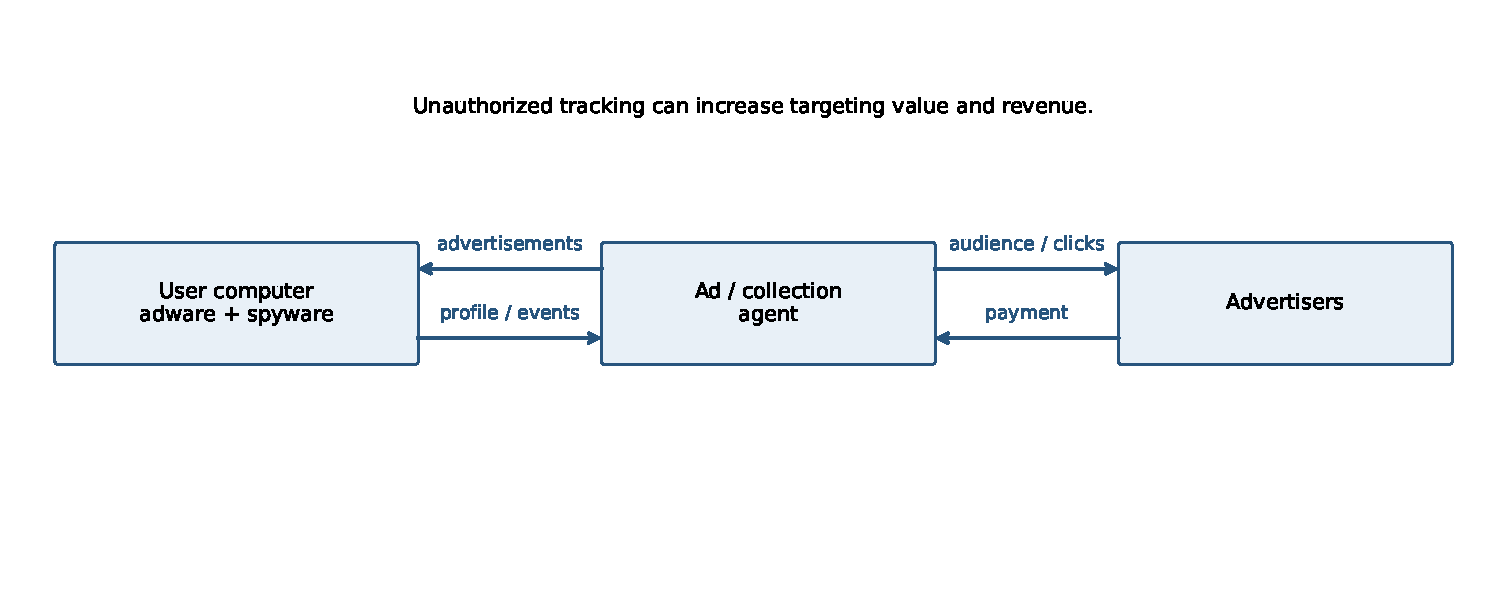
\includegraphics[width=\linewidth,height=.34\textheight,keepaspectratio]{assets/adware.pdf}
\end{center}



An installed adware component contacts an advertising agent,\allowbreak{} obtains advertisements and displays or injects them on the user's system. Advertisers pay the agent/\allowbreak{}operator for impressions,\allowbreak{} clicks or conversions.


Spyware adds collection of browsing interests,\allowbreak{} searches,\allowbreak{} application usage or other personal data. The operator can profile users,\allowbreak{} choose more profitable targeted ads and sell the data; abusive variants also steal credentials. More relevant ads can increase click/\allowbreak{}conversion revenue,\allowbreak{} explaining the incentive to combine the two components.


Keep the roles distinct: the \textbf{adware engine} displays ads,\allowbreak{} the \textbf{spyware engine} collects data,\allowbreak{} the \textbf{agent} distributes ads/\allowbreak{}receives reports,\allowbreak{} and \textbf{advertisers} fund the campaign. Not every ad-supported application secretly steals passwords; the security issue is unauthorized collection/\allowbreak{}actions and excessive privileges.




\clearpage
\subsection{A033 · 2022–23 · Q4(d)}\label{a033}

\textbf{Zero-day meaning and detection limits · 6 marks}


Original: \href{../../CSE405-Security_Merged.pdf\#page=12}{past-paper PDF p. 12}. Sitting date: 18 April 2024. Printed Section A.


\textbf{Topics:} Worm propagation,\allowbreak{} epidemic models and case studies.



\begin{quote}\small

\textbf{Question summary:} Define a zero-day attack and explain why it is dangerous.



\end{quote}


\Needspace{4\baselineskip}
{\color{ForestGreen}\textbf{Exam tip.} Distinguish “zero-day vulnerability,\allowbreak{}” “exploit” and “new malware signature.”}


A zero-day attack exploits a vulnerability before defenders have an effective available fix or established response; the issue may be unknown to the vendor. Usage varies about discovery/\allowbreak{}disclosure,\allowbreak{} so state this timing convention.


It is dangerous because patch-based prevention may be unavailable,\allowbreak{} known signatures may not match the exploit,\allowbreak{} and a widely deployed product can expose many systems before diagnosis and mitigation. Successful exploitation can give an attacker the victim process's privileges and access.


Least privilege,\allowbreak{} isolation,\allowbreak{} attack-surface reduction,\allowbreak{} memory-safety mechanisms,\allowbreak{} behavior monitoring and incident response can reduce impact even without a specific patch. Zero-day does not mean unstoppable; nor is every attack on an unpatched machine a zero-day if the patch already exists.




\clearpage
\subsection{A049 · 2021–22 · Q3(a)}\label{a049}

\textbf{DLL injection and inherited process authority · 5 marks}


Original: \href{../../CSE405-Security_Merged.pdf\#page=15}{past-paper PDF p. 15}. Sitting date: 30 October 2023. Printed Section A.


\textbf{Topics:} Rootkit cloaking,\allowbreak{} hooking and DLL injection.



\begin{quote}\small

\textbf{Question summary:} Explain why DLL injection poses high security risks.



\end{quote}

\textbf{Coverage:} related application/\allowbreak{}extension. Rootkit/\allowbreak{}API filtering and process hijacking are taught; detailed DLL-injection mechanics are not.



\Needspace{4\baselineskip}
{\color{ForestGreen}\textbf{Exam tip.} State whose privileges the code receives and how the trust boundary was crossed.}


DLL injection causes a target process to load/\allowbreak{}execute attacker-chosen library code. The injected code runs inside that process's address space and normally with its security context. It may read secrets,\allowbreak{} intercept API calls,\allowbreak{} change behavior or conceal activity behind a trusted process name.


Injection is especially serious when a less trusted actor can influence a privileged target. Loading a DLL requires some mechanism—such as already granted debugging/\allowbreak{}write access,\allowbreak{} an unsafe loading/\allowbreak{}search path or a vulnerability. The term itself does not imply any process can inject into any other process.


Use least privilege,\allowbreak{} protected loading paths,\allowbreak{} explicit trusted library resolution,\allowbreak{} integrity controls and restrictions on cross-process modification. Rootkit API filtering is one possible consequence; injection and hooking are related but not identical.




\clearpage
\subsection{A057 · 2021–22 · Q5(a)}\label{a057}

\textbf{Why sell many signature-distinct variants of one exploit? · 12 marks}


Original: \href{../../CSE405-Security_Merged.pdf\#page=16}{past-paper PDF p. 16}. Sitting date: 30 October 2023. Printed Section B.


\textbf{Topics:} Encrypted,\allowbreak{} polymorphic and metamorphic viruses; Adware,\allowbreak{} spyware and malware economics.



\begin{quote}\small

\textbf{Question summary:} Explain the financial benefits of creating many malware variants exploiting the same popular-software vulnerability but having different signatures.



\end{quote}


\Needspace{4\baselineskip}
{\color{ForestGreen}\textbf{Exam tip.} Identify the reusable cost,\allowbreak{} the cheap variation and the revenue gained from longer evasion.}


An exploit and the malware bytes delivered by it are different assets. Reusing one working exploit reduces development cost,\allowbreak{} while mutation/\allowbreak{}packing changes the payload's byte patterns and hashes. Customers can receive apparently distinct products without the author discovering a new vulnerability each time.


A new variant may evade a scanner that only recognizes older byte signatures,\allowbreak{} extending infection lifetime and increasing income from spam,\allowbreak{} fraud,\allowbreak{} credential theft or ransomware. Cheap automated variation also makes defenders analyze/\allowbreak{}update many samples,\allowbreak{} while the attacker amortizes the original exploit investment over a large vulnerable population.


This is an economic advantage rather than a proof of invisibility: patching the underlying flaw blocks all variants using it; behavioral detection,\allowbreak{} emulation and integrity controls can recognize shared effects. Polymorphism changes encrypted representations/\allowbreak{}decryptors; metamorphism rewrites the body while preserving behavior.




\clearpage
\subsection{A059 · 2021–22 · Q5(c)}\label{a059}

\textbf{Disrupting C\&C through coordinated investigation · 11 marks}


Original: \href{../../CSE405-Security_Merged.pdf\#page=16}{past-paper PDF p. 16}. Sitting date: 30 October 2023. Printed Section B.


\textbf{Topics:} Botnet creation,\allowbreak{} C\&C and malicious agents; Honeypot topology,\allowbreak{} monitoring and overhead.



\begin{quote}\small

\textbf{Question summary:} Formulate a process to take down a botnet command-and-control server.



\end{quote}


\Needspace{4\baselineskip}
{\color{ForestGreen}\textbf{Exam tip.} Include discovery,\allowbreak{} coordinated disruption and endpoint cleanup; a DoS attack on the suspected server is not a sound takedown plan.}


Observe representative malware in a contained analysis environment or honeypot; record C\&C domains/\allowbreak{}IPs,\allowbreak{} protocol,\allowbreak{} certificate/\allowbreak{}key material,\allowbreak{} connection patterns and fallback channels. Correlate evidence from multiple infections before identifying control infrastructure.


Coordinate with the responsible hosting providers,\allowbreak{} registrars,\allowbreak{} network operators and authorized response teams. Preserve evidence,\allowbreak{} arrange suspension/\allowbreak{}seizure or a controlled sinkhole of confirmed infrastructure,\allowbreak{} and prevent the replacement endpoint from becoming an attacker tool. Block validated indicators,\allowbreak{} notify affected owners and remove/\allowbreak{}rebuild infected hosts so they cannot simply reconnect elsewhere.


A centralized botnet may lose command delivery if its key server disappears. Redundant servers,\allowbreak{} domain-generation algorithms and peer-to-peer C\&C can survive a single-server action; map those dependencies and plan simultaneous disruption. Taking down a C\&C endpoint does not remove installed malware or recover stolen credentials.




\clearpage
\subsection{A069 · 2020–21 · Q1(a)}\label{a069}

\textbf{WannaCry vulnerability,\allowbreak{} success and zero-day status · 12 marks}


Original: \href{../../CSE405-Security_Merged.pdf\#page=18}{past-paper PDF p. 18}. Sitting date: 25 September 2022. Printed Section A.


\textbf{Topics:} Worm propagation,\allowbreak{} epidemic models and case studies.



\begin{quote}\small

\textbf{Question summary:} Identify WannaCry’s main vulnerability,\allowbreak{} why it succeeded and whether it was a zero-day attack.



\end{quote}


\Needspace{4\baselineskip}
{\color{ForestGreen}\textbf{Exam tip.} Give the patch-versus-outbreak timeline,\allowbreak{} not just the word “ransomware.”}


WannaCry combined ransomware with worm-like propagation through vulnerable Windows \textbf{SMBv1} services,\allowbreak{} using an exploit associated with EternalBlue. The widely observed May 2017 outbreak reached systems missing the \textbf{MS17-010} update released on \textbf{14 March 2017}.


It succeeded because many exposed/\allowbreak{}reachable systems remained unpatched,\allowbreak{} legacy systems were widespread and weak segmentation allowed lateral propagation. The payload encrypted files and demanded payment; automatic spread amplified the damage.


For that outbreak,\allowbreak{} the exploited flaw was \textbf{not a zero-day}: a fix had been available before the attacks. A newly encountered ransomware executable or unavailable local signature does not make the underlying patched vulnerability unknown.


\href{https://www.microsoft.com/en-us/security/blog/2017/05/12/wannacrypt-ransomware-worm-targets-out-of-date-systems/}{Microsoft's contemporaneous analysis},\allowbreak{} \href{https://learn.microsoft.com/en-us/security-updates/securitybulletins/2017/ms17-010}{MS17-010}.




\clearpage
\subsection{A077 · 2020–21 · Q3(c)}\label{a077}

\textbf{Derive the SI epidemic worm model · 11 marks}


Original: \href{../../CSE405-Security_Merged.pdf\#page=18}{past-paper PDF p. 18}. Sitting date: 25 September 2022. Printed Section A.


\textbf{Topics:} Worm propagation,\allowbreak{} epidemic models and case studies.



\begin{quote}\small

\textbf{Question summary:} Explain an epidemic model of worm propagation with a figure.



\end{quote}


\Needspace{4\baselineskip}
{\color{ForestGreen}\textbf{Exam tip.} Define the rate convention and explain all three phases of the S curve.}


Let \(N\) be the fixed vulnerable population,\allowbreak{} \(I(t)\) infected hosts and \(S(t)=N-I(t)\) susceptible hosts. With uniform random contact and rate constant \(\beta\),\allowbreak{} infections occur at rate



\[
\frac{dI}{dt}=\beta I S=\beta I(N-I).
\]

Separate variables and integrate:



\[
\frac{1}{N}\log\frac{I}{N-I}=\beta t+C,
\]

so for \(I(0)=I_0\),\allowbreak{}



\[
I(t)=\frac{N}{1+\left(\frac{N-I_0}{I_0}\right)e^{-\beta Nt}}.
\]

Initially \(I\ll N\) and growth is approximately exponential,\allowbreak{} \(I(t)\approx I_0e^{\beta Nt}\). Around \(I=N/2\),\allowbreak{} new infections grow fastest. Eventually few susceptible hosts remain and the curve saturates.



\begin{center}
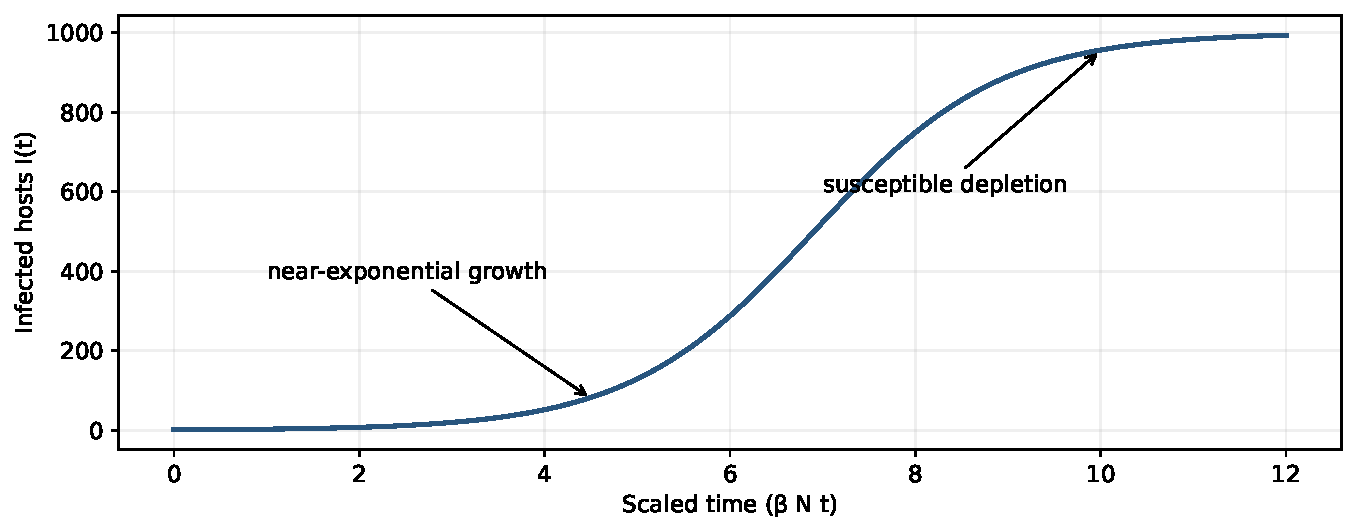
\includegraphics[width=\linewidth,height=.34\textheight,keepaspectratio]{assets/worm-growth.pdf}
\end{center}



An alternative convention defines \(\lambda=\beta N\) and writes \(dI/dt=\lambda I(1-I/N)\); do not confuse the units of the constants. Real networks violate uniform mixing and may have patching,\allowbreak{} recovery,\allowbreak{} scanning bias,\allowbreak{} congestion or disconnected hosts. The SI model here assumes no recovery during the modeled interval.




\clearpage
\subsection{A079 · 2020–21 · Q4(b)}\label{a079}

\textbf{Value and defense of an internal malware agent · 12 marks}


Original: \href{../../CSE405-Security_Merged.pdf\#page=19}{past-paper PDF p. 19}. Sitting date: 25 September 2022. Printed Section A.


\textbf{Topics:} Botnet creation,\allowbreak{} C\&C and malicious agents; Firewall state,\allowbreak{} evasion and defense limits.



\begin{quote}\small

\textbf{Question summary:} Explain why an attacker installs an agent inside a corporate network,\allowbreak{} delivery methods and prevention; assess whether a firewall can help.



\end{quote}


\Needspace{4\baselineskip}
{\color{ForestGreen}\textbf{Exam tip.} Draw the outbound connection from the inside agent; that explains why “there is a firewall” is not a complete defense.}


An internal agent provides persistence,\allowbreak{} local discovery,\allowbreak{} access to internal services,\allowbreak{} credential theft and a foothold for lateral movement. It can initiate an outbound C\&C connection,\allowbreak{} so a perimeter policy blocking only unsolicited inbound connections may not stop it.


Delivery can involve phishing attachments,\allowbreak{} malicious installers/\allowbreak{}updates,\allowbreak{} browser/\allowbreak{}application vulnerabilities or compromised credentials used to install code. The exact route determines prevention: patching,\allowbreak{} least privilege,\allowbreak{} restricted software execution,\allowbreak{} strong authentication,\allowbreak{} segmentation and endpoint monitoring are complementary controls.


A firewall helps by limiting exposed services,\allowbreak{} enforcing internal segmentation and restricting outbound destinations/\allowbreak{}protocols. It is insufficient when malicious traffic is carried over a permitted encrypted session or authorized-looking channel,\allowbreak{} and it does not clean an already compromised endpoint. Correlate endpoint and network evidence,\allowbreak{} isolate affected systems and restore trustworthy state.




\clearpage
\subsection{A092 · 2019–20 · Q2(a)}\label{a092}

\textbf{Botnet architecture and distributed floods · 12 marks}


Original: \href{../../CSE405-Security_Merged.pdf\#page=22}{past-paper PDF p. 22}. Sitting date: 07 September 2021. Printed Section A.


\textbf{Topics:} Botnet creation,\allowbreak{} C\&C and malicious agents; DoS/\allowbreak{}DDoS,\allowbreak{} reflection and resource exhaustion.



\begin{quote}\small

\textbf{Question summary:} Explain botnet components and how they launch DDoS,\allowbreak{} with a figure.



\end{quote}


\Needspace{4\baselineskip}
{\color{ForestGreen}\textbf{Exam tip.} Separate infection/\allowbreak{}agent installation,\allowbreak{} C\&C command delivery and the eventual flood payload.}


A botnet is a collection of compromised hosts running remotely controlled agents. A botmaster distributes instructions via one or more C\&C endpoints or a peer-to-peer overlay. Agents report status and execute commands,\allowbreak{} often without their owners' knowledge.



\begin{Verbatim}[breaklines=true,breakanywhere=true,fontsize=\small,frame=single,rulecolor=\color{PanelBorder}]
                    botmaster
                  /           \
              C&C 1           C&C 2
             /  |  \         /  |  \
           bot bot bot     bot bot bot
              \   \         /   /
                coordinated traffic
                        victim
\end{Verbatim}

For DDoS,\allowbreak{} many bots simultaneously send requests/\allowbreak{}packets that exhaust the victim's link,\allowbreak{} state,\allowbreak{} CPU or application capacity. Distribution increases aggregate rate and makes simple source-IP blocking costly because legitimate users can share networks with bots. Spoofing is optional: many botnet floods use the bots' real addresses.


Defend with endpoint prevention/\allowbreak{}cleanup,\allowbreak{} segmentation,\allowbreak{} C\&C disruption,\allowbreak{} rate/\allowbreak{}admission controls and upstream traffic mitigation. A perimeter filter alone cannot restore an already saturated incoming link.




\clearpage
\subsection{A095 · 2019–20 · Q3(a)}\label{a095}

\textbf{Three reasons ransomware grew during COVID-era disruption · 12 marks}


Original: \href{../../CSE405-Security_Merged.pdf\#page=22}{past-paper PDF p. 22}. Sitting date: 07 September 2021. Printed Section A.


\textbf{Topics:} Adware,\allowbreak{} spyware and malware economics; Worm propagation,\allowbreak{} epidemic models and case studies.



\begin{quote}\small

\textbf{Question summary:} Give three major reasons ransomware attacks increased during the COVID-19 pandemic.



\end{quote}

\textbf{Coverage:} related application/\allowbreak{}extension. Malware economics is taught,\allowbreak{} but COVID-specific comparative evidence is not supplied.



\Needspace{4\baselineskip}
{\color{ForestGreen}\textbf{Exam tip.} Give three different causal mechanisms rather than three examples of phishing.}


Three plausible mechanisms are:



\begin{enumerate}

\item \textbf{Expanded remote access:} hurried deployment of remote desktops/\allowbreak{}VPNs,\allowbreak{} unmanaged devices and weak authentication exposed more entry points.

\item \textbf{Social and operational disruption:} pandemic-themed phishing,\allowbreak{} overloaded support teams and delayed maintenance made initial compromise and persistence easier.

\item \textbf{Strong criminal incentives:} high dependence on online services and downtime-sensitive organizations increased payment pressure; reusable ransomware services/\allowbreak{}affiliates reduced attackers' development cost.

\end{enumerate}

These are reasoned explanations,\allowbreak{} not a quantitative causal ranking established by the supplied slides. Connect each mechanism to the attack lifecycle: entry,\allowbreak{} propagation or monetization. Defenses follow accordingly—harden remote access,\allowbreak{} authenticate strongly,\allowbreak{} maintain patches,\allowbreak{} constrain lateral movement and keep tested isolated backups.




\clearpage
\subsection{A096 · 2019–20 · Q3(b)}\label{a096}

\textbf{Encrypted-virus structure and detection · 12 marks}


Original: \href{../../CSE405-Security_Merged.pdf\#page=22}{past-paper PDF p. 22}. Sitting date: 07 September 2021. Printed Section A.


\textbf{Topics:} Encrypted,\allowbreak{} polymorphic and metamorphic viruses.



\begin{quote}\small

\textbf{Question summary:} Explain how an encrypted virus is formed and how to detect it.



\end{quote}


\Needspace{4\baselineskip}
{\color{ForestGreen}\textbf{Exam tip.} Encrypting the body changes its bytes; the decryptor is still executable code that defenders may recognize.}


A basic encrypted virus consists of a relatively fixed \textbf{decryptor/\allowbreak{}loader} plus an encrypted copy of its malicious body. At execution,\allowbreak{} the loader reconstructs the body in memory and transfers control to it. Different keys can change the ciphertext without changing the behavior.



\begin{Verbatim}[breaklines=true,breakanywhere=true,fontsize=\small,frame=single,rulecolor=\color{PanelBorder}]
on disk: [decryptor | key/derivation data | encrypted body]
run: decryptor -> plaintext body in memory -> malicious execution
\end{Verbatim}

A scanner may recognize the fixed decryptor even when the encrypted body differs. Emulation/\allowbreak{}sandbox execution can let the sample decrypt and then recognize the exposed body or behavior. Integrity baselines detect unexpected changes to legitimate files. Static heuristics may identify suspicious loading patterns but can produce false positives.


A polymorphic virus also varies its decryptor; a metamorphic virus rewrites the body itself. Emulation has time/\allowbreak{}visibility limits and can be evaded,\allowbreak{} so it is one layer rather than guaranteed detection.




\clearpage
\subsection{A112 · 2018–19 · Q1(c)}\label{a112}

\textbf{Threshold-triggered banking-data exfiltration · 9 marks}


Original: \href{../../CSE405-Security_Merged.pdf\#page=26}{past-paper PDF p. 26}. Sitting date: 24 October 2019. Printed Section A.


\textbf{Topics:} Backdoors,\allowbreak{} logic bombs and insider abuse.



\begin{quote}\small

\textbf{Question summary:} A programmer secretly emails account details whenever a balance exceeds USD 5,\allowbreak{}000. Identify the attack and risks.



\end{quote}


\Needspace{4\baselineskip}
{\color{ForestGreen}\textbf{Exam tip.} Identify actor,\allowbreak{} trigger and payload separately rather than assigning a label without explaining the violation.}


This is an \textbf{insider-planted malicious feature} with a condition-triggered payload. The balance threshold is a logic-bomb-style trigger; emailing private account information is a confidentiality violation. It can also be described as a Trojanized banking application because normal banking behavior conceals the malicious action. It is not necessarily a backdoor unless it also provides an unauthorized access/\allowbreak{}bypass mechanism.


Risks include theft of customer financial data,\allowbreak{} fraud targeting,\allowbreak{} regulatory/\allowbreak{}contractual exposure and loss of trust. The program's ordinary database/\allowbreak{}email privileges may make the action appear legitimate to coarse controls.


Use independent code review,\allowbreak{} separation of development/\allowbreak{}deployment authority,\allowbreak{} least-privilege database/\allowbreak{}mail access,\allowbreak{} controlled builds and monitoring for unusual outbound data. Maintain protected audit records so a privileged developer cannot erase the evidence easily.




\clearpage
\subsection{A114 · 2018–19 · Q2(a)}\label{a114}

\textbf{Polymorphic versus metamorphic viruses with examples · 7 marks}


Original: \href{../../CSE405-Security_Merged.pdf\#page=26}{past-paper PDF p. 26}. Sitting date: 24 October 2019. Printed Section A.


\textbf{Topics:} Encrypted,\allowbreak{} polymorphic and metamorphic viruses.



\begin{quote}\small

\textbf{Question summary:} Distinguish polymorphic and metamorphic viruses and give two examples of each.



\end{quote}


\Needspace{4\baselineskip}
{\color{ForestGreen}\textbf{Exam tip.} “Changes its signature” describes both. State whether the body itself is rewritten.}


A \textbf{polymorphic} virus varies its encrypted representation and often its decryptor while reconstructing substantially the same body at runtime. \textbf{Metamorphic} malware rewrites the body itself using equivalent instruction sequences,\allowbreak{} register changes,\allowbreak{} code permutation or junk insertion,\allowbreak{} so there need not be a constant decrypted body to recognize.


Historical examples commonly analyzed as polymorphic include \textbf{1260} and \textbf{Marburg}; metamorphic examples include \textbf{W32/\allowbreak{}Simile (Etap)} and \textbf{Win95/\allowbreak{}Regswap}. Families can combine techniques,\allowbreak{} so the mechanism is a more reliable distinction than a rigid label.


Polymorphic detection can emulate the decryptor and inspect the recovered body; metamorphic detection may require normalization,\allowbreak{} semantic/\allowbreak{}behavioral analysis and broader heuristics. Neither kind guarantees evasion against patching or behavior-based containment.


\href{https://www.f-secure.com/v-descs/marburg}{Marburg analysis},\allowbreak{} \href{https://www.virusbulletin.com/virusbulletin/2006/03/solving-metamorphic-puzzle}{metamorphic analysis}.




\clearpage
\subsection{A115 · 2018–19 · Q2(b)}\label{a115}

\textbf{Why adware authors add spyware · 8 marks}


Original: \href{../../CSE405-Security_Merged.pdf\#page=26}{past-paper PDF p. 26}. Sitting date: 24 October 2019. Printed Section A.


\textbf{Topics:} Adware,\allowbreak{} spyware and malware economics.



\begin{quote}\small

\textbf{Question summary:} Explain why spyware benefits an adware author.



\end{quote}


\Needspace{4\baselineskip}
{\color{ForestGreen}\textbf{Exam tip.} Label both the money flow and the information flow.}



\begin{center}
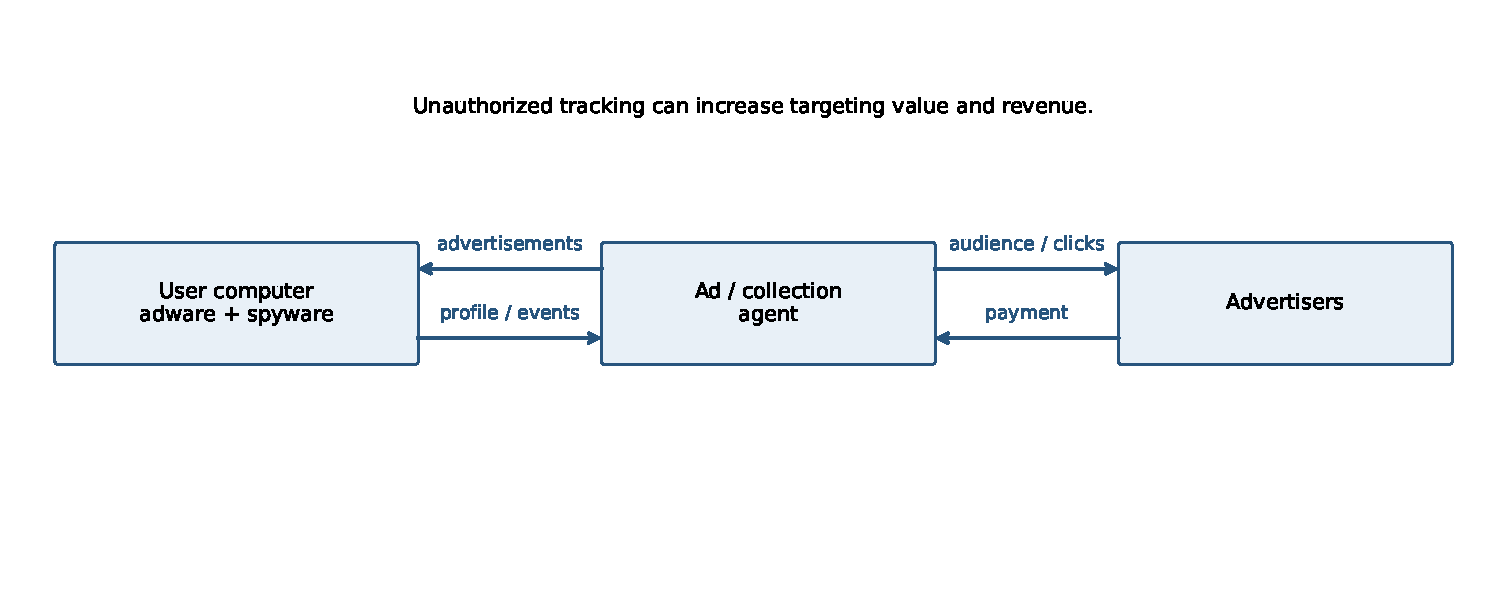
\includegraphics[width=\linewidth,height=.34\textheight,keepaspectratio]{assets/adware.pdf}
\end{center}



An installed adware component contacts an advertising agent,\allowbreak{} obtains advertisements and displays or injects them on the user's system. Advertisers pay the agent/\allowbreak{}operator for impressions,\allowbreak{} clicks or conversions.


Spyware adds collection of browsing interests,\allowbreak{} searches,\allowbreak{} application usage or other personal data. The operator can profile users,\allowbreak{} choose more profitable targeted ads and sell the data; abusive variants also steal credentials. More relevant ads can increase click/\allowbreak{}conversion revenue,\allowbreak{} explaining the incentive to combine the two components.


Keep the roles distinct: the \textbf{adware engine} displays ads,\allowbreak{} the \textbf{spyware engine} collects data,\allowbreak{} the \textbf{agent} distributes ads/\allowbreak{}receives reports,\allowbreak{} and \textbf{advertisers} fund the campaign. Not every ad-supported application secretly steals passwords; the security issue is unauthorized collection/\allowbreak{}actions and excessive privileges.




\clearpage
\subsection{A116 · 2018–19 · Q2(c)}\label{a116}

\textbf{Function hooking and three concealment targets · 12 marks}


Original: \href{../../CSE405-Security_Merged.pdf\#page=26}{past-paper PDF p. 26}. Sitting date: 24 October 2019. Printed Section A.


\textbf{Topics:} Rootkit cloaking,\allowbreak{} hooking and DLL injection.



\begin{quote}\small

\textbf{Question summary:} Define rootkit function hooking,\allowbreak{} its danger and three examples of avoiding detection.



\end{quote}


\Needspace{4\baselineskip}
{\color{ForestGreen}\textbf{Exam tip.} Draw the intercepted query path and distinguish hooking from direct structure modification.}


A rootkit provides concealment/\allowbreak{}persistence for other malicious activity. It can hide processes,\allowbreak{} files,\allowbreak{} services,\allowbreak{} registry entries,\allowbreak{} ports or user accounts. It is distinct from the payload it hides.


In a kernel hook,\allowbreak{} privileged malicious code redirects a kernel query's dispatch path or alters its result. For example:



\begin{Verbatim}[breaklines=true,breakanywhere=true,fontsize=\small,frame=single,rulecolor=\color{PanelBorder}]
process-list tool -> system query -> hooked enumeration routine
                                  -> remove malicious process record
                                  -> return a plausible filtered list
\end{Verbatim}

The process may keep executing while ordinary tools report it absent. File/\allowbreak{}directory and network enumeration can be filtered similarly. Installing a kernel hook normally needs elevated privileges or a separate privilege-escalation vulnerability. A user-mode API hook affects fewer observation paths; \textbf{DKOM} instead directly alters kernel bookkeeping structures and need not hook the query itself.


Detect with cross-view comparisons,\allowbreak{} integrity checks and trusted offline examination. A compromised kernel can lie to tools running under it,\allowbreak{} so ordinary successful antivirus output is not proof of a clean system. Recover from trusted media and rebuild when confidence cannot be restored.


Three concrete filtered observations are: (1) omit a malicious process from process enumeration; (2) hide its files in directory/\allowbreak{}file queries; (3) omit its listening port from network-connection queries. A service/\allowbreak{}registry query can be filtered too. These are concealment examples; they do not make all independent observation paths disappear.




\clearpage
\subsection{A117 · 2018–19 · Q2(d)}\label{a117}

\textbf{Morris worm speed and consequences · 8 marks}


Original: \href{../../CSE405-Security_Merged.pdf\#page=26}{past-paper PDF p. 26}. Sitting date: 24 October 2019. Printed Section A.


\textbf{Topics:} Worm propagation,\allowbreak{} epidemic models and case studies.



\begin{quote}\small

\textbf{Question summary:} Why did the Morris worm spread rapidly and what were the consequences?



\end{quote}


\Needspace{4\baselineskip}
{\color{ForestGreen}\textbf{Exam tip.} Include reinfection/\allowbreak{}resource exhaustion,\allowbreak{} not just “it exploited a buffer overflow.”}


The 1988 Morris worm used several propagation routes,\allowbreak{} including a \texttt{fingerd} buffer overflow,\allowbreak{} a Sendmail debugging facility,\allowbreak{} trusted remote execution and password guessing. Multiple routes expanded the susceptible population,\allowbreak{} and automatic replication avoided the need for each new user to launch an attachment.


Its reinfection behavior caused repeated copies to run on already affected hosts. The resulting process/\allowbreak{}load growth exhausted resources and disrupted services across many connected systems,\allowbreak{} even without a conventional file-destruction payload. Widespread connectivity,\allowbreak{} trust relationships and weak/\allowbreak{}unpatched services amplified the effect.


The malware slides distinguish propagation vectors from payload: rapid scanning/\allowbreak{}replication is the spread mechanism; overload and loss of service are the damage.




\clearpage
\subsection{A118 · 2018–19 · Q3(a)}\label{a118}

\textbf{Easter egg versus logic bomb · 6 marks}


Original: \href{../../CSE405-Security_Merged.pdf\#page=26}{past-paper PDF p. 26}. Sitting date: 24 October 2019. Printed Section A.


\textbf{Topics:} Backdoors,\allowbreak{} logic bombs and insider abuse.



\begin{quote}\small

\textbf{Question summary:} Give examples of an Easter egg and a logic bomb.



\end{quote}


\Needspace{4\baselineskip}
{\color{ForestGreen}\textbf{Exam tip.} Name the trigger and action for the logic bomb.}


An \textbf{Easter egg} is a hidden,\allowbreak{} usually benign feature activated by an unusual input sequence—for example,\allowbreak{} a secret credits screen in a game. Hidden functionality still needs review because it may violate policy or introduce defects.


A \textbf{logic bomb} executes malicious behavior when a condition is met—for example,\allowbreak{} deleting project files on a chosen date or when a programmer's name disappears from payroll. It may lie dormant until its trigger occurs.


Both can be deliberately hidden; the essential distinction is the intended harmful action and trigger,\allowbreak{} not whether ordinary users know the feature exists. A backdoor specifically creates an unauthorized access/\allowbreak{}bypass path and need not be identical to either example.




\clearpage
\subsection{A121 · 2018–19 · Q3(d)}\label{a121}

\textbf{Bot creation,\allowbreak{} control and uses · 10 marks}


Original: \href{../../CSE405-Security_Merged.pdf\#page=26}{past-paper PDF p. 26}. Sitting date: 24 October 2019. Printed Section A.


\textbf{Topics:} Botnet creation,\allowbreak{} C\&C and malicious agents.



\begin{quote}\small

\textbf{Question summary:} Explain botnet creation/\allowbreak{}control and possible activities.



\end{quote}


\Needspace{4\baselineskip}
{\color{ForestGreen}\textbf{Exam tip.} Separate infection/\allowbreak{}agent installation,\allowbreak{} C\&C command delivery and the eventual flood payload.}


A botnet is a collection of compromised hosts running remotely controlled agents. A botmaster distributes instructions via one or more C\&C endpoints or a peer-to-peer overlay. Agents report status and execute commands,\allowbreak{} often without their owners' knowledge.



\begin{Verbatim}[breaklines=true,breakanywhere=true,fontsize=\small,frame=single,rulecolor=\color{PanelBorder}]
                    botmaster
                  /           \
              C&C 1           C&C 2
             /  |  \         /  |  \
           bot bot bot     bot bot bot
              \   \         /   /
                coordinated traffic
                        victim
\end{Verbatim}

For DDoS,\allowbreak{} many bots simultaneously send requests/\allowbreak{}packets that exhaust the victim's link,\allowbreak{} state,\allowbreak{} CPU or application capacity. Distribution increases aggregate rate and makes simple source-IP blocking costly because legitimate users can share networks with bots. Spoofing is optional: many botnet floods use the bots' real addresses.


Defend with endpoint prevention/\allowbreak{}cleanup,\allowbreak{} segmentation,\allowbreak{} C\&C disruption,\allowbreak{} rate/\allowbreak{}admission controls and upstream traffic mitigation. A perimeter filter alone cannot restore an already saturated incoming link.


Other bot activities include spam,\allowbreak{} click fraud,\allowbreak{} credential/\allowbreak{}key logging and distributing additional malware. A P2P overlay can replace a single central C\&C hierarchy and make disruption more difficult.



\clearpage
\section{Network Security}

Primary deck: \href{../slides/Ch05-NetworkSecurity.pdf}{Ch05-NetworkSecurity.\allowbreak{}pdf}




\subsection{A004 · 2023–24 · Q2(a)}\label{a004}

\textbf{Rogue DHCP gateway and MITM with the correct gateway · 10 marks}


Original: \href{../../CSE405-Security_Merged.pdf\#page=3}{past-paper PDF p. 3}. Sitting date: 06 September 2025. Printed Section A.


\textbf{Topics:} DHCP starvation,\allowbreak{} spoofing and defenses; ARP spoofing,\allowbreak{} MITM and detection.



\begin{quote}\small

\textbf{Question summary:} Attacker IP is 10.10.10.32; router/\allowbreak{}DHCP server is 10.10.10.4. Give a forged client IP/\allowbreak{}default router for Alice. If the correct router is supplied,\allowbreak{} explain another way to become MITM.



\end{quote}


\Needspace{4\baselineskip}
{\color{ForestGreen}\textbf{Exam tip.} IP addresses choose routing destinations; Ethernet MAC addresses choose local next hops. Explain both when the real gateway IP is retained.}


Offer an unused host address on the same subnet,\allowbreak{} for example \textbf{10.10.10.33},\allowbreak{} and default router \textbf{10.10.10.32} (the attacker). The mask must make both reachable—for example /\allowbreak{}24 if consistent with the real network. Do not assign Alice an address already used by the router or attacker.


Alice then sends off-subnet packets to the attacker. To maintain a working connection,\allowbreak{} the attacker forwards them to 10.10.10.4. Routing/\allowbreak{}NAT or reverse-path manipulation is needed for replies to pass through the attacker as well; merely receiving outbound packets does not automatically provide a bidirectional MITM.


If the forged offer gives the correct router,\allowbreak{} use \textbf{ARP poisoning}: tell Alice that 10.10.10.4 has the attacker's MAC,\allowbreak{} and tell the router that Alice's IP has the attacker's MAC. Forward between the two. A malicious DNS-server option can instead redirect selected hostname traffic,\allowbreak{} but does not inherently intercept every connection and does not defeat properly validated TLS.



\begin{center}
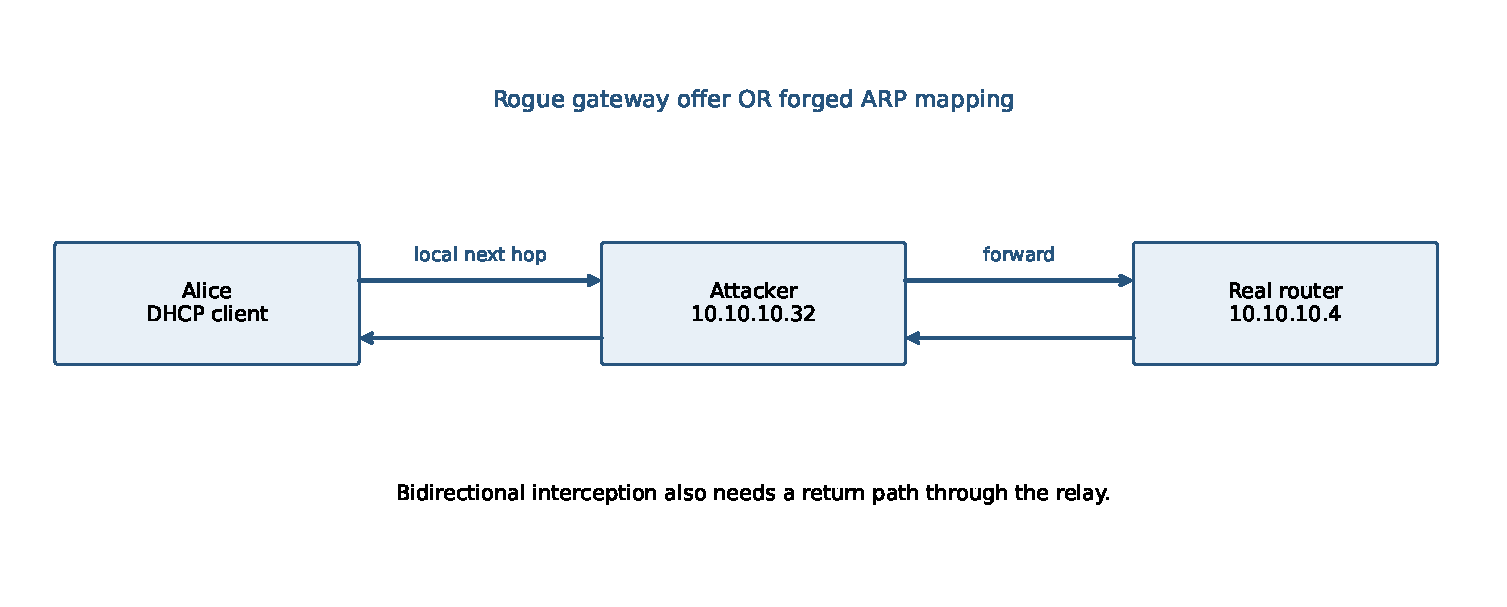
\includegraphics[width=\linewidth,height=.34\textheight,keepaspectratio]{assets/lan-mitm.pdf}
\end{center}



Defend with DHCP snooping (server replies only from trusted ports),\allowbreak{} request rate limits,\allowbreak{} binding-based dynamic ARP inspection and authenticated application protocols.




\clearpage
\subsection{A006 · 2023–24 · Q2(c)}\label{a006}

\textbf{Off-path TCP injection and establishing a replacement connection · 15 marks}


Original: \href{../../CSE405-Security_Merged.pdf\#page=3}{past-paper PDF p. 3}. Sitting date: 06 September 2025. Printed Section A.


\textbf{Topics:} TCP hijacking,\allowbreak{} spoofed segments and optimistic ACKs.



\begin{quote}\small

\textbf{Question summary:} Using the printed TCP diagram (continued on p. 4),\allowbreak{} evaluate malicious actions by an off-path attacker and impersonating the client after it resets the connection.



\end{quote}

\textbf{Coverage:} related application/\allowbreak{}extension. The network deck covers TCP state/\allowbreak{}hijacking; the modern blind-reset and ISN details extend it.



\Needspace{4\baselineskip}
{\color{ForestGreen}\textbf{Exam tip.} Separate “can spoof a packet,\allowbreak{}” “TCP accepts it,\allowbreak{}” and “application accepts the identity.” They are three different claims.}


An off-path attacker normally cannot see \(X,Y\),\allowbreak{} the ephemeral client port,\allowbreak{} or current windows. The diagram's symbolic sequence numbers are explanatory; they are \textbf{not an address leak to the attacker}. Spoofing the client's IP is insufficient to inject accepted bytes reliably.


If the tuple and current numbers become known or predictable,\allowbreak{} a client-to-server injected segment after DATA C needs the next client sequence number



\[
q=X+1+L_A+L_C,
\]

and an ACK consistent with received server bytes,\allowbreak{} initially \(Y+1+L_B\). Acceptance also depends on the receive window,\allowbreak{} TCP state and later traffic. A guessed in-window RST may disrupt legacy implementations; exact-sequence validation/\allowbreak{}challenge ACKs make blind resets harder. Flooding remains possible without successful hijacking.


For a \textbf{new} spoofed connection,\allowbreak{} the attacker can send a SYN under the client's source IP,\allowbreak{} but the server's SYN-ACK goes to the real client. To complete the handshake,\allowbreak{} the attacker must learn or predict the new server ISN and acknowledge it,\allowbreak{} and deal with the real client's resets. A prior connection's \(Y\) does not generally predict the next ISN. If the server authenticates clients at the application/\allowbreak{}TLS layer,\allowbreak{} a successful TCP handshake is still not authenticated impersonation.


Thus no reliable replacement-connection attack follows from the stated off-path capability alone. State additional assumptions if describing the classic predictable-ISN attack.




\clearpage
\subsection{A010 · 2023–24 · Q4(a)}\label{a010}

\textbf{UDP chargen/\allowbreak{}echo feedback versus TCP handshake · 10 marks}


Original: \href{../../CSE405-Security_Merged.pdf\#page=5}{past-paper PDF p. 5}. Sitting date: 06 September 2025. Printed Section A.


\textbf{Topics:} DoS/\allowbreak{}DDoS,\allowbreak{} reflection and resource exhaustion; TCP hijacking,\allowbreak{} spoofed segments and optimistic ACKs.



\begin{quote}\small

\textbf{Question summary:} JULY on UDP port 36 returns 36–360 random characters; PROTIDHONI on port 5 echoes its input. Give one empty UDP packet creating a feedback loop between X and Y,\allowbreak{} then assess a single spoofed TCP SYN when both services require a handshake.



\end{quote}


\Needspace{4\baselineskip}
{\color{ForestGreen}\textbf{Exam tip.} Trace every reply's source and destination ports. UDP has no handshake gate; TCP application services do.}


Send the empty UDP datagram with:



{\small\setlength{\tabcolsep}{3pt}
\begin{longtable}{>{\raggedright\arraybackslash}p{0.63270\linewidth}>{\raggedright\arraybackslash}p{0.33819\linewidth}}
\toprule
\textbf{Field} & \textbf{Value} \\
\midrule
\endhead
Source IP /\allowbreak{} port & Y /\allowbreak{} 5 \\
Destination IP /\allowbreak{} port & X /\allowbreak{} 36 \\
\bottomrule
\end{longtable}
}

X sends random characters back to Y:5. Y echoes them to X:36,\allowbreak{} provoking another random response,\allowbreak{} and so on. Both services consume bandwidth without further attacker packets,\allowbreak{} assuming they answer these requests indefinitely and packets continue to arrive. Reflection and application feedback create the problem; source spoofing hides the initiating sender.


With TCP,\allowbreak{} a single spoofed SYN does \textbf{not} create the same application-data loop. The recipient sends SYN-ACK to the spoofed peer,\allowbreak{} which has no matching connection and typically sends RST (or drops it). No three-way handshake/\allowbreak{}application request has completed. Since the attacker is off-path,\allowbreak{} it cannot generally learn the server sequence number needed to complete a forged handshake. There are therefore no magic seq/\allowbreak{}ACK values satisfying the requested one-SYN attack under the stated assumptions.


Prevent feedback by disabling unused services,\allowbreak{} refusing inappropriate service-to-service responses,\allowbreak{} limiting rates and applying source-address validation.




\clearpage
\subsection{A022 · 2022–23 · Q1(b)}\label{a022}

\textbf{SYN backlog exhaustion and cookie validation · 12 marks}


Original: \href{../../CSE405-Security_Merged.pdf\#page=11}{past-paper PDF p. 11}. Sitting date: 18 April 2024. Printed Section A.


\textbf{Topics:} SYN flooding and stateless SYN cookies.



\begin{quote}\small

\textbf{Question summary:} Explain SYN flooding with a figure and evaluate SYN cookies.



\end{quote}


\Needspace{4\baselineskip}
{\color{ForestGreen}\textbf{Exam tip.} Explain exactly when state is allocated and why returning the cookie is evidence of receiving the SYN-ACK.}


A normal TCP listener reserves state for a half-open connection after SYN and awaits the final ACK. Many incomplete handshakes can fill its backlog and deny legitimate clients.



\begin{center}
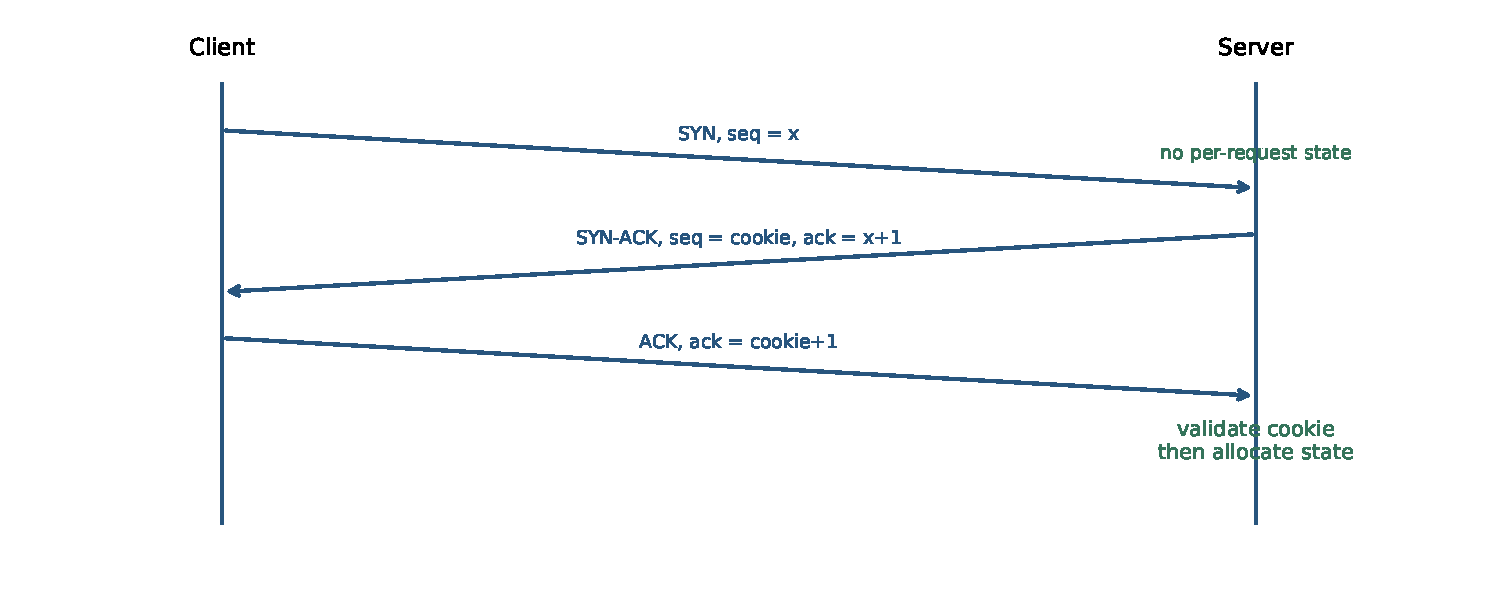
\includegraphics[width=\linewidth,height=.34\textheight,keepaspectratio]{assets/syn-cookie.pdf}
\end{center}



Instead of storing each request,\allowbreak{} the server chooses an initial sequence number encoding a short time value,\allowbreak{} supported parameters and a secret-dependent authenticator of the flow tuple. It sends SYN-ACK with this cookie and ACK equal to client ISN plus one. When the client returns ACK,\allowbreak{} the server checks \textbf{ACK−1},\allowbreak{} recomputes the authenticator for recent time slots,\allowbreak{} and allocates connection state only after validation.


Conceptually:



\[
c=\operatorname{Encode}\left(t,\mathrm{options},\operatorname{TruncMAC}_K(\mathrm{srcIP},\mathrm{srcPort},\mathrm{dstIP},\mathrm{dstPort},t,\mathrm{options})\right).
\]

The real cookie fits within the 32-bit TCP ISN,\allowbreak{} so authentication bits and options are limited. The secret is not sent to clients. A blind spoofing sender generally cannot see and return a correct cookie. An on-path adversary can,\allowbreak{} and attackers with genuine addresses can still complete handshakes and consume resources.


Cookies protect half-open \textbf{state},\allowbreak{} not an already saturated link,\allowbreak{} all CPU costs,\allowbreak{} or application floods. Historical slide statements about OS support/\allowbreak{}options are not universal claims about current implementations.


\href{https://www.rfc-editor.org/rfc/rfc4987}{Reference: RFC 4987}.




\clearpage
\subsection{A023 · 2022–23 · Q1(c)}\label{a023}

\textbf{DHCP starvation message flow and rogue-server relationship · 13 marks}


Original: \href{../../CSE405-Security_Merged.pdf\#page=11}{past-paper PDF p. 11}. Sitting date: 18 April 2024. Printed Section A.


\textbf{Topics:} DHCP starvation,\allowbreak{} spoofing and defenses.



\begin{quote}\small

\textbf{Question summary:} Explain DHCP starvation with a message diagram and analyze its relation to DHCP spoofing.



\end{quote}


\Needspace{4\baselineskip}
{\color{ForestGreen}\textbf{Exam tip.} Label starvation as DoS and rogue configuration as a separate trust failure.}


Normal allocation follows \textbf{DISCOVER → OFFER → REQUEST → ACK}. A client broadcasts discovery; a server offers a lease; the client selects it; the server acknowledges.


In starvation,\allowbreak{} an attacker presents many invented client identities and completes enough allocation exchanges to occupy the available lease pool. Legitimate new clients then receive no usable lease. Many DISCOVERs alone may consume pending offers temporarily,\allowbreak{} but a complete explanation includes lease commitment/\allowbreak{}retention behavior.



\begin{Verbatim}[breaklines=true,breakanywhere=true,fontsize=\small,frame=single,rulecolor=\color{PanelBorder}]
invented client i  -> server: DISCOVER
server            -> client: OFFER address i
invented client i  -> server: REQUEST address i
server            -> client: ACK lease i
repeat until the allocatable pool is exhausted
\end{Verbatim}

A rogue DHCP server can then offer an attacker-controlled gateway or DNS resolver to clients the legitimate server cannot serve. This \textbf{spoofing/\allowbreak{}MITM} phase is distinct from starvation's availability failure; spoofing can also succeed by winning a race without first exhausting the pool.


Use DHCP snooping with trusted server ports,\allowbreak{} rate limits on untrusted client ports,\allowbreak{} identity/\allowbreak{}lease limits and monitoring for abnormal allocation churn. Port-security limits alone may not cover all DHCP client-identifier variations.




\clearpage
\subsection{A027 · 2022–23 · Q3(a)}\label{a027}

\textbf{CAM exhaustion and switch behavior · 12 marks}


Original: \href{../../CSE405-Security_Merged.pdf\#page=11}{past-paper PDF p. 11}. Sitting date: 18 April 2024. Printed Section A.


\textbf{Topics:} Switch MAC-table flooding and port security.



\begin{quote}\small

\textbf{Question summary:} Explain MAC flooding with topology,\allowbreak{} effects on a switch and attacker benefits.



\end{quote}


\Needspace{4\baselineskip}
{\color{ForestGreen}\textbf{Exam tip.} Explain source learning and destination lookup separately; exhausting an ARP cache is a different attack.}


A switch learns \textbf{source MAC → ingress port} bindings in its finite CAM/\allowbreak{}FDB table. An attacker sends frames with many fabricated source MACs,\allowbreak{} exhausting or churning that table.



\begin{center}
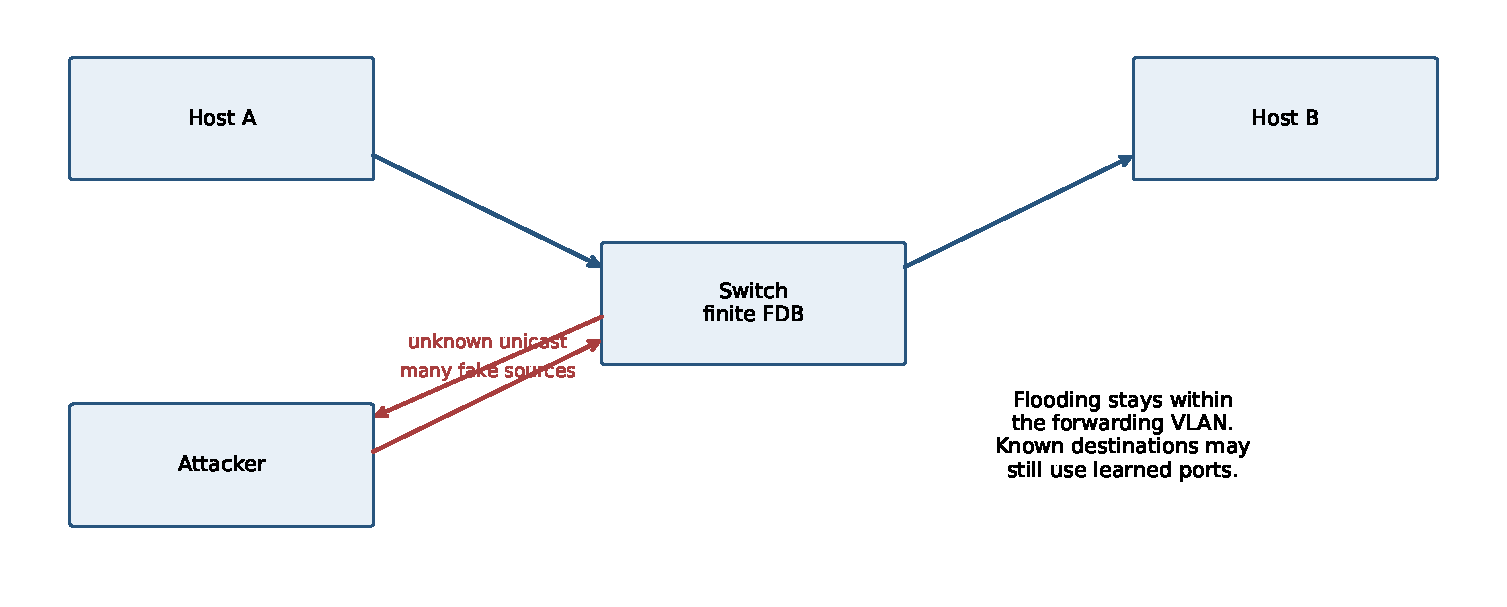
\includegraphics[width=\linewidth,height=.34\textheight,keepaspectratio]{assets/switch-flood.pdf}
\end{center}



When a destination MAC is unknown,\allowbreak{} ordinary switching may flood that frame to other forwarding ports \textbf{within its VLAN}. The attacker can then see traffic that would otherwise have been unicast elsewhere,\allowbreak{} and excessive flooding may cause congestion. This does not universally turn the device into a hub: existing known destinations may still be forwarded correctly,\allowbreak{} hardware behavior varies and VLAN boundaries remain relevant.


Use port-security MAC limits,\allowbreak{} appropriate violation actions,\allowbreak{} source controls,\allowbreak{} segmentation and unknown-unicast limits. Monitor abnormal source churn/\allowbreak{}FDB pressure. End-to-end encryption protects contents even if frames are copied. DAI addresses forged ARP bindings and is not a complete substitute for CAM-source limits.




\clearpage
\subsection{A060 · 2021–22 · Q6(a)}\label{a060}

\textbf{Detect optimistic ACKs by withholding a segment · 12 marks}


Original: \href{../../CSE405-Security_Merged.pdf\#page=17}{past-paper PDF p. 17}. Sitting date: 30 October 2023. Printed Section B.


\textbf{Topics:} TCP hijacking,\allowbreak{} spoofed segments and optimistic ACKs.



\begin{quote}\small

\textbf{Question summary:} Explain how randomly dropping data segments at the sender helps detect optimistic TCP ACK attacks.



\end{quote}

\textbf{Coverage:} related application/\allowbreak{}extension. The network deck explains TCP ACK state; optimistic-ACK probing is beyond its explicit treatment.



\Needspace{4\baselineskip}
{\color{ForestGreen}\textbf{Exam tip.} “Randomly drop packets” is incomplete: explain the impossible acknowledgment that supplies evidence.}


An optimistic receiver ACKs bytes it has not received,\allowbreak{} tricking a sender into increasing its congestion window and sending faster than the path can carry. An attacker can abuse this to amplify offered traffic.


The proposed sender defense secretly \textbf{withholds} a chosen segment before it ever enters the network and tracks the resulting byte gap. Suppose bytes 1000–1999 are withheld while later segments arrive. A correct cumulative ACK cannot advance beyond 1000 until those missing bytes have actually been transmitted and received (ACK numbers denote the next expected byte).


A receiver that acknowledges 3000 while the gap still exists claims receipt of bytes the sender never sent. The sender can flag/\allowbreak{}terminate or restrict that flow. Random selection makes it harder for a blind ACK generator to predict the probes. Merely observing network loss is weaker because retransmission/\allowbreak{}reordering can explain later ACKs; track exactly what was intentionally withheld and when retransmission becomes possible.


This is the historical proposed modification in the question,\allowbreak{} not an assumption that all TCP stacks implement it. It must account for legitimate cumulative ACK/\allowbreak{}SACK behavior and imposes some performance cost.


\href{https://drum.lib.umd.edu/items/d435007a-3809-4c75-8e4f-85ae20c5d5e7}{Primary study},\allowbreak{} \href{https://www.kb.cert.org/vuls/id/102014}{CERT vulnerability note}.




\clearpage
\subsection{A063 · 2021–22 · Q7(a)}\label{a063}

\textbf{SYN-cookie defense · 12 marks}


Original: \href{../../CSE405-Security_Merged.pdf\#page=17}{past-paper PDF p. 17}. Sitting date: 30 October 2023. Printed Section B.


\textbf{Topics:} SYN flooding and stateless SYN cookies.



\begin{quote}\small

\textbf{Question summary:} Explain how SYN cookies defend against SYN flooding.



\end{quote}


\Needspace{4\baselineskip}
{\color{ForestGreen}\textbf{Exam tip.} Explain exactly when state is allocated and why returning the cookie is evidence of receiving the SYN-ACK.}


A normal TCP listener reserves state for a half-open connection after SYN and awaits the final ACK. Many incomplete handshakes can fill its backlog and deny legitimate clients.



\begin{center}
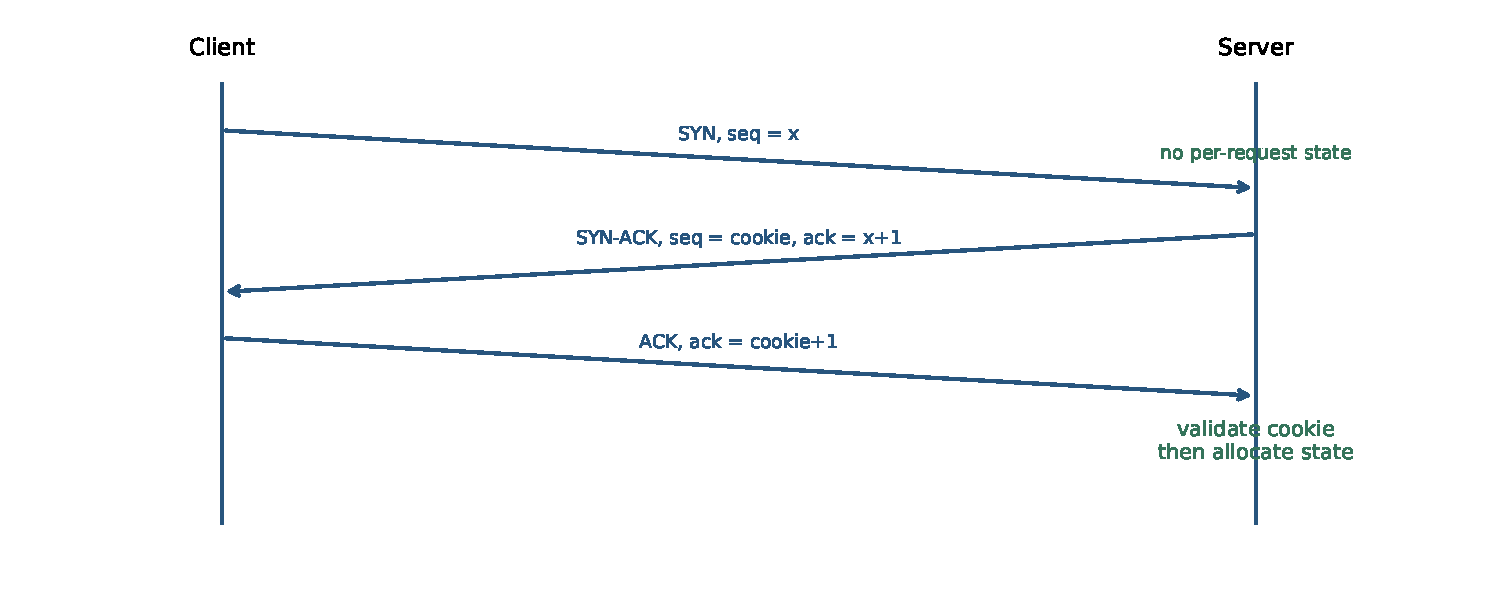
\includegraphics[width=\linewidth,height=.34\textheight,keepaspectratio]{assets/syn-cookie.pdf}
\end{center}



Instead of storing each request,\allowbreak{} the server chooses an initial sequence number encoding a short time value,\allowbreak{} supported parameters and a secret-dependent authenticator of the flow tuple. It sends SYN-ACK with this cookie and ACK equal to client ISN plus one. When the client returns ACK,\allowbreak{} the server checks \textbf{ACK−1},\allowbreak{} recomputes the authenticator for recent time slots,\allowbreak{} and allocates connection state only after validation.


Conceptually:



\[
c=\operatorname{Encode}\left(t,\mathrm{options},\operatorname{TruncMAC}_K(\mathrm{srcIP},\mathrm{srcPort},\mathrm{dstIP},\mathrm{dstPort},t,\mathrm{options})\right).
\]

The real cookie fits within the 32-bit TCP ISN,\allowbreak{} so authentication bits and options are limited. The secret is not sent to clients. A blind spoofing sender generally cannot see and return a correct cookie. An on-path adversary can,\allowbreak{} and attackers with genuine addresses can still complete handshakes and consume resources.


Cookies protect half-open \textbf{state},\allowbreak{} not an already saturated link,\allowbreak{} all CPU costs,\allowbreak{} or application floods. Historical slide statements about OS support/\allowbreak{}options are not universal claims about current implementations.


\href{https://www.rfc-editor.org/rfc/rfc4987}{Reference: RFC 4987}.




\clearpage
\subsection{A078 · 2020–21 · Q4(a)}\label{a078}

\textbf{ARP prevention,\allowbreak{} monitoring and locating the attacking port · 12 marks}


Original: \href{../../CSE405-Security_Merged.pdf\#page=19}{past-paper PDF p. 19}. Sitting date: 25 September 2022. Printed Section A.


\textbf{Topics:} ARP spoofing,\allowbreak{} MITM and detection.



\begin{quote}\small

\textbf{Question summary:} Give ARP-spoofing defenses and ways to identify an attacking host on the internal network.



\end{quote}


\Needspace{4\baselineskip}
{\color{ForestGreen}\textbf{Exam tip.} Separate detecting a bad binding from attributing it to a physical port/\allowbreak{}device.}


ARP maps an IPv4 next-hop address to an Ethernet MAC without strong native authentication. Forged replies can tell a victim that the gateway's IP belongs to the attacker and tell the gateway the inverse lie,\allowbreak{} creating a forwarding MITM.


Prevent with DHCP-snooping-derived \textbf{dynamic ARP inspection},\allowbreak{} carefully maintained static bindings for small critical environments,\allowbreak{} appropriate switch access controls and authenticated end-to-end protocols. Encryption protects payloads but does not remove false local routing or DoS.


Monitor ARP changes,\allowbreak{} duplicate claims for one IP,\allowbreak{} unusual gratuitous replies and binding conflicts using packet capture/\allowbreak{}ARPwatch-style tools. Compare with legitimate DHCP leases,\allowbreak{} inventory and known gateway MACs. Then correlate the suspicious MAC with the switch forwarding table,\allowbreak{} ingress-port counters and physical/\allowbreak{}802.1X identity to find its access port; isolate according to the response plan.


A single MAC serving several IPs is an indicator rather than proof: routers,\allowbreak{} virtualization and failover can do that legitimately. MACs can also be spoofed; do not equate a packet's source string with a trustworthy person identity.




\clearpage
\subsection{A099 · 2019–20 · Q4(b)}\label{a099}

\textbf{Making a switch flood unknown destinations · 12 marks}


Original: \href{../../CSE405-Security_Merged.pdf\#page=23}{past-paper PDF p. 23}. Sitting date: 07 September 2021. Printed Section A.


\textbf{Topics:} Switch MAC-table flooding and port security.



\begin{quote}\small

\textbf{Question summary:} Why make a switch behave like a hub,\allowbreak{} what attack does this and how can it be prevented?



\end{quote}


\Needspace{4\baselineskip}
{\color{ForestGreen}\textbf{Exam tip.} Explain source learning and destination lookup separately; exhausting an ARP cache is a different attack.}


A switch learns \textbf{source MAC → ingress port} bindings in its finite CAM/\allowbreak{}FDB table. An attacker sends frames with many fabricated source MACs,\allowbreak{} exhausting or churning that table.



\begin{center}
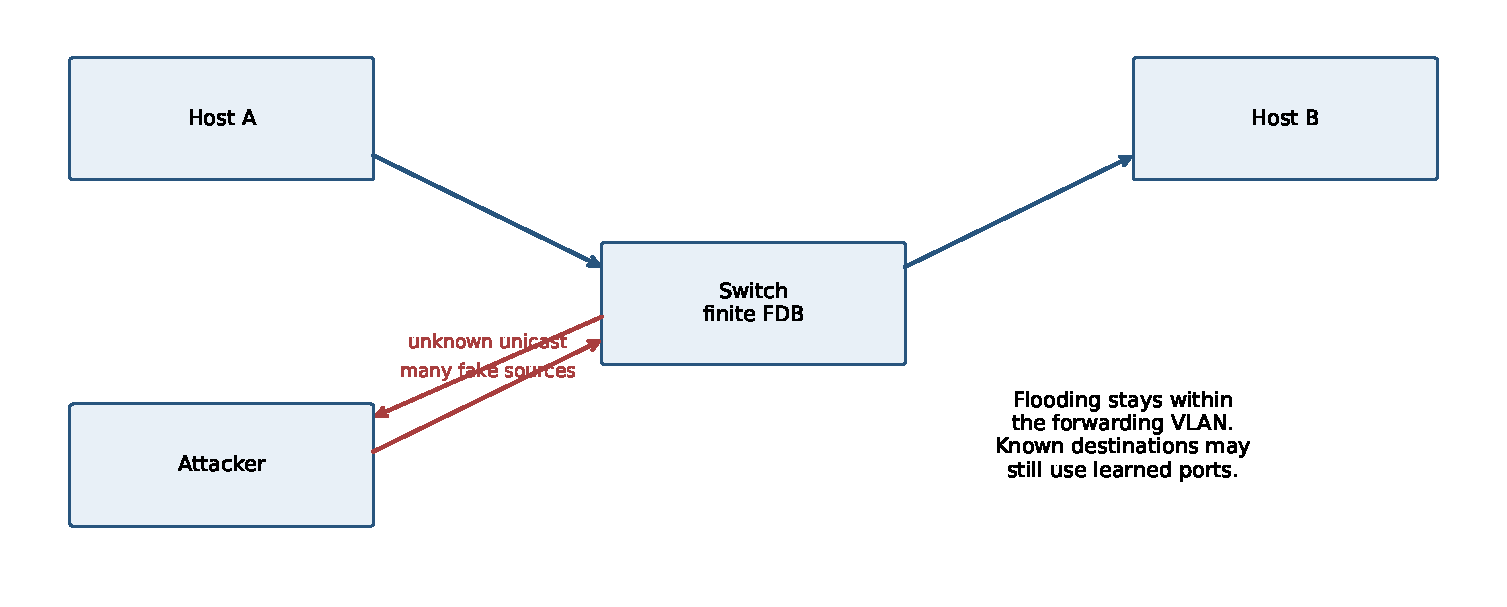
\includegraphics[width=\linewidth,height=.34\textheight,keepaspectratio]{assets/switch-flood.pdf}
\end{center}



When a destination MAC is unknown,\allowbreak{} ordinary switching may flood that frame to other forwarding ports \textbf{within its VLAN}. The attacker can then see traffic that would otherwise have been unicast elsewhere,\allowbreak{} and excessive flooding may cause congestion. This does not universally turn the device into a hub: existing known destinations may still be forwarded correctly,\allowbreak{} hardware behavior varies and VLAN boundaries remain relevant.


Use port-security MAC limits,\allowbreak{} appropriate violation actions,\allowbreak{} source controls,\allowbreak{} segmentation and unknown-unicast limits. Monitor abnormal source churn/\allowbreak{}FDB pressure. End-to-end encryption protects contents even if frames are copied. DAI addresses forged ARP bindings and is not a complete substitute for CAM-source limits.




\clearpage
\subsection{A100 · 2019–20 · Q4(c)}\label{a100}

\textbf{Withheld-segment detection of optimistic ACKs · 11 marks}


Original: \href{../../CSE405-Security_Merged.pdf\#page=23}{past-paper PDF p. 23}. Sitting date: 07 September 2021. Printed Section A.


\textbf{Topics:} TCP hijacking,\allowbreak{} spoofed segments and optimistic ACKs.



\begin{quote}\small

\textbf{Question summary:} Explain with examples how sender-side random segment dropping detects optimistic ACKs.



\end{quote}

\textbf{Coverage:} related application/\allowbreak{}extension. Optimistic-ACK details extend the TCP-state slides.



\Needspace{4\baselineskip}
{\color{ForestGreen}\textbf{Exam tip.} “Randomly drop packets” is incomplete: explain the impossible acknowledgment that supplies evidence.}


An optimistic receiver ACKs bytes it has not received,\allowbreak{} tricking a sender into increasing its congestion window and sending faster than the path can carry. An attacker can abuse this to amplify offered traffic.


The proposed sender defense secretly \textbf{withholds} a chosen segment before it ever enters the network and tracks the resulting byte gap. Suppose bytes 1000–1999 are withheld while later segments arrive. A correct cumulative ACK cannot advance beyond 1000 until those missing bytes have actually been transmitted and received (ACK numbers denote the next expected byte).


A receiver that acknowledges 3000 while the gap still exists claims receipt of bytes the sender never sent. The sender can flag/\allowbreak{}terminate or restrict that flow. Random selection makes it harder for a blind ACK generator to predict the probes. Merely observing network loss is weaker because retransmission/\allowbreak{}reordering can explain later ACKs; track exactly what was intentionally withheld and when retransmission becomes possible.


This is the historical proposed modification in the question,\allowbreak{} not an assumption that all TCP stacks implement it. It must account for legitimate cumulative ACK/\allowbreak{}SACK behavior and imposes some performance cost.


\href{https://drum.lib.umd.edu/items/d435007a-3809-4c75-8e4f-85ae20c5d5e7}{Primary study},\allowbreak{} \href{https://www.kb.cert.org/vuls/id/102014}{CERT vulnerability note}.




\clearpage
\subsection{A119 · 2018–19 · Q3(b)}\label{a119}

\textbf{Complete TCP hijacking · 9 marks}


Original: \href{../../CSE405-Security_Merged.pdf\#page=26}{past-paper PDF p. 26}. Sitting date: 24 October 2019. Printed Section A.


\textbf{Topics:} TCP hijacking,\allowbreak{} spoofed segments and optimistic ACKs; ARP spoofing,\allowbreak{} MITM and detection.



\begin{quote}\small

\textbf{Question summary:} Explain with a diagram how to perform TCP session hijacking.



\end{quote}


\Needspace{4\baselineskip}
{\color{ForestGreen}\textbf{Exam tip.} Separate observing numbers,\allowbreak{} injecting acceptable bytes and silencing conflicting legitimate traffic.}


An attacker first needs the connection tuple and sequence/\allowbreak{}window state. A practical on-LAN route in the lecture is ARP poisoning,\allowbreak{} which makes the attacker a forwarding intermediary:



\begin{Verbatim}[breaklines=true,breakanywhere=true,fontsize=\small,frame=single,rulecolor=\color{PanelBorder}]
client <----> attacker relay <----> server
             observe seq/ACK
             suppress/replace selected packets
\end{Verbatim}

Track bytes in both directions. To impersonate the client,\allowbreak{} a forged segment must use the client's source IP/\allowbreak{}port,\allowbreak{} server destination and an acceptable next sequence number/\allowbreak{}ACK. Its TCP checksum must match. If the real client continues sending conflicting stream data,\allowbreak{} the session can desynchronize or terminate; full takeover requires controlling/\allowbreak{}suppressing that competing traffic,\allowbreak{} not merely inserting one arbitrary packet.


Correct authenticated application encryption prevents accepted malicious \textbf{application content} without the session keys,\allowbreak{} although an on-path attacker may still disrupt availability. Random ISNs and blind-injection defenses help against off-path guessing but do not hide state from an on-path observer.




\clearpage
\subsection{A120 · 2018–19 · Q3(c)}\label{a120}

\textbf{Optimistic TCP ACK mechanism and mitigation · 10 marks}


Original: \href{../../CSE405-Security_Merged.pdf\#page=26}{past-paper PDF p. 26}. Sitting date: 24 October 2019. Printed Section A.


\textbf{Topics:} TCP hijacking,\allowbreak{} spoofed segments and optimistic ACKs.



\begin{quote}\small

\textbf{Question summary:} Define optimistic TCP ACK attack and give mitigations.



\end{quote}

\textbf{Coverage:} related application/\allowbreak{}extension. The deck covers TCP state but not optimistic-ACK algorithms.



\Needspace{4\baselineskip}
{\color{ForestGreen}\textbf{Exam tip.} “Randomly drop packets” is incomplete: explain the impossible acknowledgment that supplies evidence.}


An optimistic receiver ACKs bytes it has not received,\allowbreak{} tricking a sender into increasing its congestion window and sending faster than the path can carry. An attacker can abuse this to amplify offered traffic.


The proposed sender defense secretly \textbf{withholds} a chosen segment before it ever enters the network and tracks the resulting byte gap. Suppose bytes 1000–1999 are withheld while later segments arrive. A correct cumulative ACK cannot advance beyond 1000 until those missing bytes have actually been transmitted and received (ACK numbers denote the next expected byte).


A receiver that acknowledges 3000 while the gap still exists claims receipt of bytes the sender never sent. The sender can flag/\allowbreak{}terminate or restrict that flow. Random selection makes it harder for a blind ACK generator to predict the probes. Merely observing network loss is weaker because retransmission/\allowbreak{}reordering can explain later ACKs; track exactly what was intentionally withheld and when retransmission becomes possible.


This is the historical proposed modification in the question,\allowbreak{} not an assumption that all TCP stacks implement it. It must account for legitimate cumulative ACK/\allowbreak{}SACK behavior and imposes some performance cost.


\href{https://drum.lib.umd.edu/items/d435007a-3809-4c75-8e4f-85ae20c5d5e7}{Primary study},\allowbreak{} \href{https://www.kb.cert.org/vuls/id/102014}{CERT vulnerability note}.


Complementary mitigations include sensible pacing/\allowbreak{}traffic shaping and per-client resource limits; they reduce amplification but do not themselves prove receipt of every byte. The withheld-segment test specifically targets false receipt claims.



\clearpage
\section{DNS Security}

Primary deck: \href{../slides/Ch06-1-NetworkDNS.pdf}{Ch06-1-NetworkDNS.\allowbreak{}pdf}




\subsection{A009 · 2023–24 · Q3(c)}\label{a009}

\textbf{Kaminsky retries,\allowbreak{} bailiwick,\allowbreak{} DNS-over-TLS and DNSSEC · 20 marks}


Original: \href{../../CSE405-Security_Merged.pdf\#page=4}{past-paper PDF p. 4}. Sitting date: 06 September 2025. Printed Section A.


\textbf{Topics:} DNS poisoning,\allowbreak{} Kaminsky races,\allowbreak{} pharming and DNSSEC.



\begin{quote}\small

\textbf{Question summary:} An internal attacker loads many fakeN.\allowbreak{}buet.\allowbreak{}ac.\allowbreak{}bd image names to poison the shared resolver (no source-port randomization). Explain why many images help,\allowbreak{} whether the same page can poison www.\allowbreak{}google.\allowbreak{}com,\allowbreak{} and the effects of DNS-over-TLS and DNSSEC.



\end{quote}


\Needspace{4\baselineskip}
{\color{ForestGreen}\textbf{Exam tip.} Identify which zone the forged record concerns and which network hop each defense actually protects.}


Each fresh random subdomain forces a cache miss and creates another response race. The attacker attempts to match the outstanding query's name/\allowbreak{}type/\allowbreak{}class,\allowbreak{} transaction ID and socket tuple before the authoritative response arrives. A forged in-bailiwick delegation/\allowbreak{}NS response can try to redirect subsequent resolution for the parent zone. Repeating fresh names avoids waiting for one cached answer's TTL to expire.


For \(q\) independent races with per-race win probability \(p\):



\[
P(\text{at least one win})=1-(1-p)^q.
\]

If \(r\) distinct ID guesses fit in a race and the only unknown is a uniform 16-bit ID,\allowbreak{} \(p\approx \min(r,2^{16})/2^{16}\). Sending all IDs helps only if they arrive in time. Do not apply an unrestricted \(q r/2^{16}\) formula when names,\allowbreak{} sockets or implementation query coalescing prevent cross-matching.


The listed \texttt{fakeN.\allowbreak{}buet.\allowbreak{}ac.\allowbreak{}bd} queries do \textbf{not} authorize replacement of \texttt{google.\allowbreak{}com} data. A resolver enforcing bailiwick/\allowbreak{}trust rules discards unrelated additional records. Targeting another domain requires corresponding outstanding queries and an applicable poisoning opportunity; “all DNS is cached together” is insufficient.


\textbf{DNS over TLS depends on the hop.} Authenticating/\allowbreak{}encrypting the client-to-recursive-resolver connection prevents tampering on that link,\allowbreak{} but does not secure a separate UDP recursive-to-authoritative race. Authenticated protection of the attacked hop would stop network forgery there.


\textbf{DNSSEC} validates signed RRsets through DNSKEY/\allowbreak{}DS and a configured trust anchor. Forged answer/\allowbreak{}delegation data fails signature/\allowbreak{}chain validation for a securely signed zone. An untrusted key bundled in the answer is not a trust anchor. DNSSEC does not conceal queries or guarantee availability.



\begin{center}
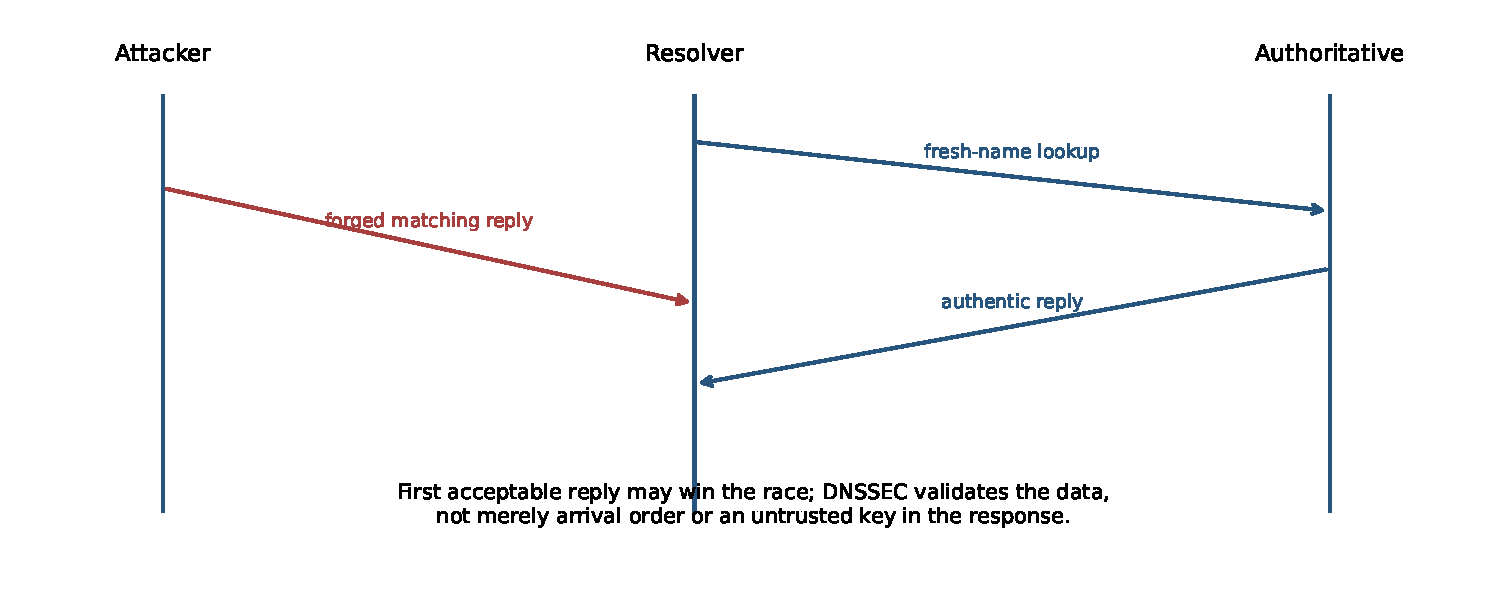
\includegraphics[width=\linewidth,height=.34\textheight,keepaspectratio]{assets/dns-race.pdf}
\end{center}



\href{https://www.rfc-editor.org/rfc/rfc5452}{Reference: RFC 5452},\allowbreak{} \href{https://www.rfc-editor.org/rfc/rfc4033}{DNSSEC introduction: RFC 4033}.




\clearpage
\subsection{A030 · 2022–23 · Q4(a)}\label{a030}

\textbf{DNS cache poisoning and three defenses · 12 marks}


Original: \href{../../CSE405-Security_Merged.pdf\#page=12}{past-paper PDF p. 12}. Sitting date: 18 April 2024. Printed Section A.


\textbf{Topics:} DNS poisoning,\allowbreak{} Kaminsky races,\allowbreak{} pharming and DNSSEC.



\begin{quote}\small

\textbf{Question summary:} Define DNS cache poisoning,\allowbreak{} explain exploitation and provide three defenses.



\end{quote}


\Needspace{4\baselineskip}
{\color{ForestGreen}\textbf{Exam tip.} Give a defense against the exact forgery path; “use a firewall” alone does not authenticate DNS data.}


A resolver stores a forged name/\allowbreak{}delegation mapping and later serves it as cached truth. Clients may be redirected to an attacker's server or denied service. An off-path attacker commonly forces an uncached lookup and races a guessed response against the authoritative reply.


The forged response must match the outstanding query's transaction ID,\allowbreak{} name/\allowbreak{}type/\allowbreak{}class,\allowbreak{} addresses and ports and satisfy record-trust/\allowbreak{}bailiwick rules. A 16-bit predictable identifier or fixed source port makes guessing easier. A cached malicious delegation can affect many subsequent names.


Three complementary defenses are:



\begin{enumerate}

\item \textbf{Unpredictable transaction IDs and per-query source ports:} enlarge the guessing space; keep entropy through NAT/\allowbreak{}firewalls.

\item \textbf{Strict response and bailiwick validation:} reject mismatched/\allowbreak{}unsolicited responses and unrelated additional records; restrict recursion to intended clients and patch resolver flaws.

\item \textbf{DNSSEC validation:} verify signed RRsets through authenticated delegation to a trust anchor. Reject bogus data for securely signed zones.

\end{enumerate}

Restricting recursion alone does not protect against an internal attacker or a browser-triggered lookup. DNSSEC provides authenticity/\allowbreak{}integrity,\allowbreak{} not encryption or total DoS prevention.



\begin{center}
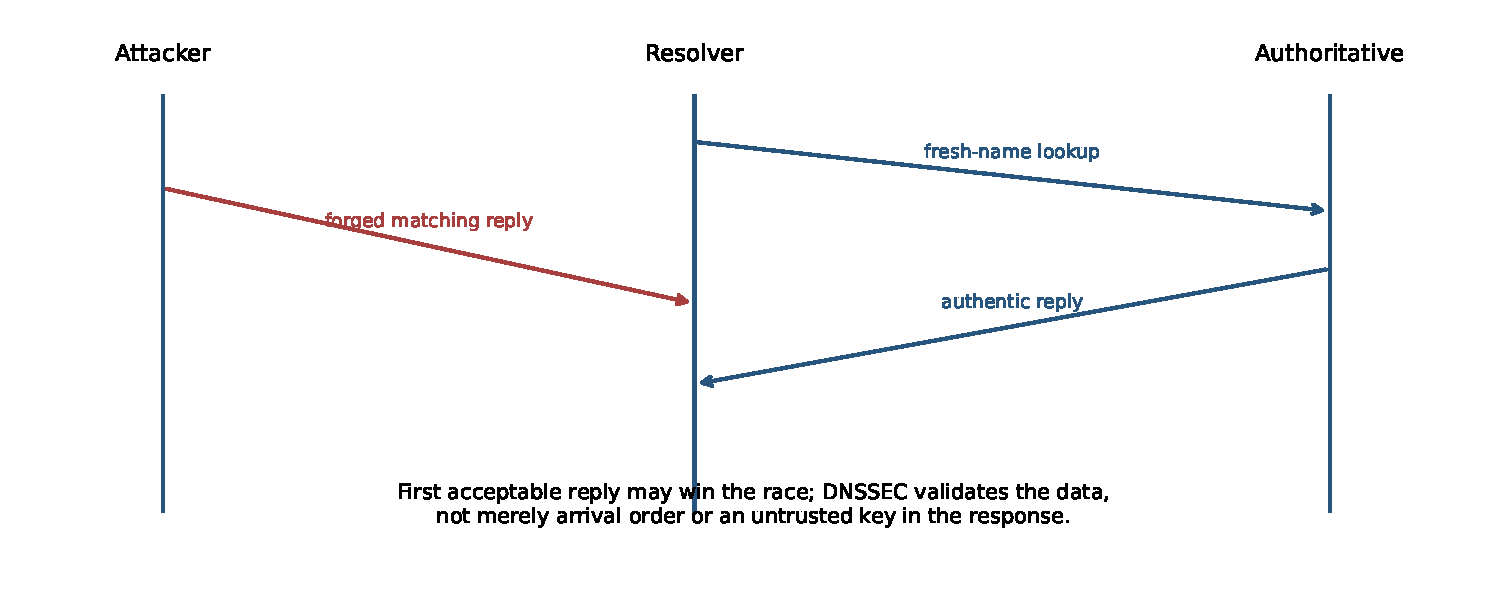
\includegraphics[width=\linewidth,height=.34\textheight,keepaspectratio]{assets/dns-race.pdf}
\end{center}



\href{https://www.rfc-editor.org/rfc/rfc5452}{Reference: RFC 5452}.




\clearpage
\subsection{A061 · 2021–22 · Q6(b)}\label{a061}

\textbf{Three DNS poisoning countermeasures · 12 marks}


Original: \href{../../CSE405-Security_Merged.pdf\#page=17}{past-paper PDF p. 17}. Sitting date: 30 October 2023. Printed Section B.


\textbf{Topics:} DNS poisoning,\allowbreak{} Kaminsky races,\allowbreak{} pharming and DNSSEC.



\begin{quote}\small

\textbf{Question summary:} Design three mechanisms to prevent or mitigate DNS cache poisoning.



\end{quote}


\Needspace{4\baselineskip}
{\color{ForestGreen}\textbf{Exam tip.} Give a defense against the exact forgery path; “use a firewall” alone does not authenticate DNS data.}


A resolver stores a forged name/\allowbreak{}delegation mapping and later serves it as cached truth. Clients may be redirected to an attacker's server or denied service. An off-path attacker commonly forces an uncached lookup and races a guessed response against the authoritative reply.


The forged response must match the outstanding query's transaction ID,\allowbreak{} name/\allowbreak{}type/\allowbreak{}class,\allowbreak{} addresses and ports and satisfy record-trust/\allowbreak{}bailiwick rules. A 16-bit predictable identifier or fixed source port makes guessing easier. A cached malicious delegation can affect many subsequent names.


Three complementary defenses are:



\begin{enumerate}

\item \textbf{Unpredictable transaction IDs and per-query source ports:} enlarge the guessing space; keep entropy through NAT/\allowbreak{}firewalls.

\item \textbf{Strict response and bailiwick validation:} reject mismatched/\allowbreak{}unsolicited responses and unrelated additional records; restrict recursion to intended clients and patch resolver flaws.

\item \textbf{DNSSEC validation:} verify signed RRsets through authenticated delegation to a trust anchor. Reject bogus data for securely signed zones.

\end{enumerate}

Restricting recursion alone does not protect against an internal attacker or a browser-triggered lookup. DNSSEC provides authenticity/\allowbreak{}integrity,\allowbreak{} not encryption or total DoS prevention.



\begin{center}
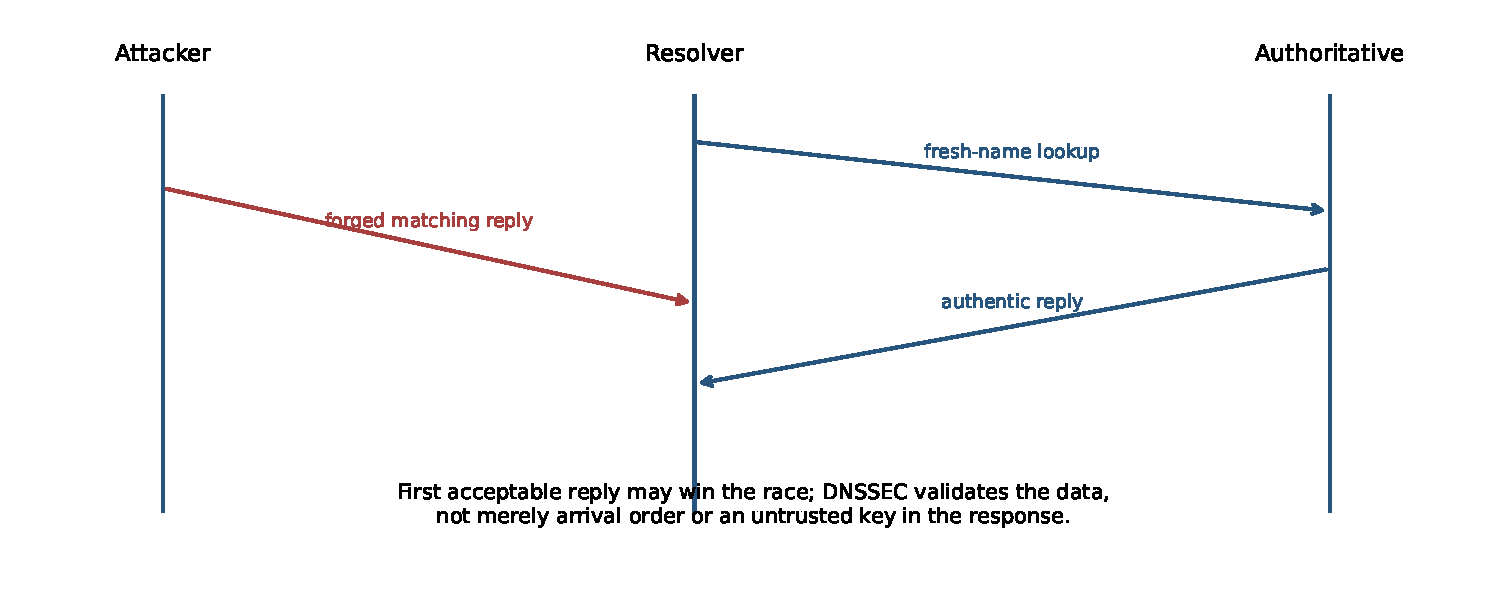
\includegraphics[width=\linewidth,height=.34\textheight,keepaspectratio]{assets/dns-race.pdf}
\end{center}



\href{https://www.rfc-editor.org/rfc/rfc5452}{Reference: RFC 5452}.




\clearpage
\subsection{A098 · 2019–20 · Q4(a)}\label{a098}

\textbf{DNS redirection as a MITM precursor · 12 marks}


Original: \href{../../CSE405-Security_Merged.pdf\#page=23}{past-paper PDF p. 23}. Sitting date: 07 September 2021. Printed Section A.


\textbf{Topics:} DNS poisoning,\allowbreak{} Kaminsky races,\allowbreak{} pharming and DNSSEC.



\begin{quote}\small

\textbf{Question summary:} Explain with a diagram how DNS spoofing can launch MITM.



\end{quote}


\Needspace{4\baselineskip}
{\color{ForestGreen}\textbf{Exam tip.} Explain the additional trust failure needed to turn DNS poisoning into interception of validated HTTPS.}



\begin{Verbatim}[breaklines=true,breakanywhere=true,fontsize=\small,frame=single,rulecolor=\color{PanelBorder}]
client asks resolver: bank.example address?
forged/corrupted answer: attacker IP
client -> attacker proxy -> real bank
client <- attacker proxy <- real bank
\end{Verbatim}

The attacker replaces a hostname's expected address,\allowbreak{} receives the client's connection and proxies to the real service while observing/\allowbreak{}modifying unprotected traffic. A local forged answer or poisoned recursive cache can supply the wrong mapping. To be MITM,\allowbreak{} the attacker must forward both sides rather than merely show an unrelated fake page.


Correct HTTPS hostname/\allowbreak{}certificate validation prevents a DNS redirect alone from authenticating the attacker as \texttt{bank.\allowbreak{}example}: it lacks the trusted corresponding server key. It may still cause failure/\allowbreak{}DoS,\allowbreak{} exploit a user overriding warnings or succeed with a separately compromised certificate/\allowbreak{}key. DNSSEC validation addresses signed DNS authenticity; authenticated TLS independently binds the server identity.




\clearpage
\subsection{A122 · 2018–19 · Q4(a)}\label{a122}

\textbf{Random-subdomain cache-poisoning advantage · 10 marks}


Original: \href{../../CSE405-Security_Merged.pdf\#page=26}{past-paper PDF p. 26}. Sitting date: 24 October 2019. Printed Section A.


\textbf{Topics:} DNS poisoning,\allowbreak{} Kaminsky races,\allowbreak{} pharming and DNSSEC.



\begin{quote}\small

\textbf{Question summary:} Why use subdomain DNS cache poisoning,\allowbreak{} and why can it succeed more readily than simple poisoning?



\end{quote}


\Needspace{4\baselineskip}
{\color{ForestGreen}\textbf{Exam tip.} Explain the two advantages separately: repeated cache misses and a valuable cached delegation target.}


A simple repeated query for one name may hit a cached answer,\allowbreak{} leaving no new authoritative response race until TTL expiry. Random fresh subdomains such as \texttt{nonce1.example},\allowbreak{} \texttt{nonce2.example} repeatedly cause cache misses.


For each outstanding lookup,\allowbreak{} the attacker races forged replies carrying an applicable delegation/\allowbreak{}NS change for the target zone. A successful accepted delegation can redirect later lookups beyond that one fresh name. New names provide many attempts without waiting for the original host record to expire.


Success still requires matching the actual query identifiers/\allowbreak{}socket and satisfying resolver trust/\allowbreak{}bailiwick rules. This is not permission to insert arbitrary records for unrelated domains,\allowbreak{} and a correct DNSSEC-validating resolver rejects forged data for a securely signed zone. Unpredictable IDs/\allowbreak{}source ports,\allowbreak{} strict validation and resolver updates reduce the race opportunity.




\clearpage
\subsection{A123 · 2018–19 · Q4(b)}\label{a123}

\textbf{DNS redirection in a pharming-versus-phishing comparison · 8 printed marks (mixed question)}


Original: \href{../../CSE405-Security_Merged.pdf\#page=26}{past-paper PDF p. 26}. Sitting date: 24 October 2019. Printed Section A.


\textbf{Topics:} DNS poisoning,\allowbreak{} Kaminsky races,\allowbreak{} pharming and DNSSEC.



\begin{quote}\small

\textbf{Question summary:} Explain the DNS-redirection (pharming) side of the printed comparison,\allowbreak{} with an example.



\end{quote}

\textbf{Sec A scope:} Covers the DNS/\allowbreak{}pharming component of the printed comparison. The phishing topic is assigned to Sec B. The printed 8 marks are for the complete comparison,\allowbreak{} not this component alone.


\textbf{Coverage:} related application/\allowbreak{}extension. Only the Sec A DNS/\allowbreak{}pharming component is developed here; the standalone phishing topic remains in Sec B.



\Needspace{4\baselineskip}
{\color{ForestGreen}\textbf{Exam tip.} Locate the altered mapping or resolver configuration. A fake-looking URL alone is not evidence of DNS poisoning.}


\textbf{Pharming} redirects a legitimate hostname to an attacker-controlled destination by changing a trusted-looking name-resolution path. For example,\allowbreak{} a poisoned resolver cache maps \texttt{bank.\allowbreak{}example} to the attacker's address. A user can type the correct hostname and still reach that address; this distinguishes DNS redirection from a lure persuading the user to visit a deceptive hostname.


Trace the Sec A mechanism:



\begin{Verbatim}[breaklines=true,breakanywhere=true,fontsize=\small,frame=single,rulecolor=\color{PanelBorder}]
user requests correct hostname -> resolver returns poisoned mapping
                              -> client connects to attacker address
\end{Verbatim}

A poisoned hosts file,\allowbreak{} rogue resolver configuration or compromised router can produce a similar redirection. Use protected resolver configuration,\allowbreak{} validated DNS responses/\allowbreak{}DNSSEC where applicable and correctly authenticated endpoint connections. A DNS change alone does not supply the trusted server's private key or defeat proper certificate validation; denial of service may still occur.



\clearpage
\section{Firewalls,\allowbreak{} Tunneling and IDS}

Primary deck: \href{../slides/Ch06-2-FW-Tunneling-IDS-REDUCED.pdf}{Ch06-2-FW-Tunneling-IDS-REDUCED.\allowbreak{}pdf}




\subsection{A007 · 2023–24 · Q3(a)}\label{a007}

\textbf{Can NIDS/\allowbreak{}firewall plus HTTPS always stop the network attacks? · 10 printed marks (mixed question)}


Original: \href{../../CSE405-Security_Merged.pdf\#page=4}{past-paper PDF p. 4}. Sitting date: 06 September 2025. Printed Section A.


\textbf{Topics:} Firewall state,\allowbreak{} evasion and defense limits; TCP hijacking,\allowbreak{} spoofed segments and optimistic ACKs; SYN flooding and stateless SYN cookies; DNS poisoning,\allowbreak{} Kaminsky races,\allowbreak{} pharming and DNSSEC; DoS/\allowbreak{}DDoS,\allowbreak{} reflection and resource exhaustion.



\begin{quote}\small

\textbf{Question summary:} An HTTPS-only server farm has a NIDS and firewall processing incoming requests. With an on-path attacker,\allowbreak{} assess the Sec A cases: RST injection,\allowbreak{} SYN flooding,\allowbreak{} DNS spoofing and DDoS.



\end{quote}

\textbf{Sec A scope:} Covers the four network-defense cases. The reflected-XSS case in the original five-part question belongs to Sec B and is excluded. The 10 printed marks cover all five cases; no per-case allocation is supplied.



\Needspace{4\baselineskip}
{\color{ForestGreen}\textbf{Exam tip.} Place each attack at its layer: link/\allowbreak{}IP,\allowbreak{} TCP,\allowbreak{} TLS or application. A protection at one layer need not authenticate the others.}


\textbf{No blanket guarantee follows from this setup.} A NIDS may only alert; a firewall's effectiveness depends on its policy,\allowbreak{} visibility and resources.



{\small\setlength{\tabcolsep}{3pt}
\begin{longtable}{>{\raggedright\arraybackslash}p{0.30002\linewidth}>{\raggedright\arraybackslash}p{0.67087\linewidth}}
\toprule
\textbf{Attack} & \textbf{Reason and relevant defense} \\
\midrule
\endhead
RST injection & TLS authenticates records,\allowbreak{} not ordinary TCP headers. An on-path adversary can observe sequence state and attempt a valid reset. State checks/\allowbreak{}TCP-level authentication can help; HTTPS alone does not authenticate RSTs. \\
SYN flooding & SYNs reach the server before TLS. SYN cookies/\allowbreak{}proxies and upstream limits reduce backlog exhaustion,\allowbreak{} but not all link saturation. \\
DNS spoofing & HTTPS certificate validation can stop successful server impersonation when DNS redirects to an unauthenticated server. It does not prevent poisoning itself or resulting denial of service. DNSSEC validation addresses signed DNS data. \\
DDoS & A firewall may filter attack traffic but cannot recover bandwidth already exhausted upstream. Distributed mitigation,\allowbreak{} capacity and application limits are needed. \\
\bottomrule
\end{longtable}
}



\clearpage
\subsection{A011 · 2023–24 · Q4(b)}\label{a011}

\textbf{TCP segmentation,\allowbreak{} reassembly and limits of a guaranteed evasion · 10 marks}


Original: \href{../../CSE405-Security_Merged.pdf\#page=5}{past-paper PDF p. 5}. Sitting date: 06 September 2025. Printed Section A.


\textbf{Topics:} Firewall state,\allowbreak{} evasion and defense limits.



\begin{quote}\small

\textbf{Question summary:} A smart stateful firewall blocks bytes spelling admin and allows everything else. Mallory splits the word into five packets sent out of order. Will that evade the rule? If not,\allowbreak{} propose a guaranteed strategy.



\end{quote}

\textbf{Coverage:} related application/\allowbreak{}extension. The deck distinguishes filter types; stream normalization and the impossibility of an unconditional guarantee are extensions.



\Needspace{4\baselineskip}
{\color{ForestGreen}\textbf{Exam tip.} State the inspection model first. “Stateful” does not automatically mean complete application parsing,\allowbreak{} and “encrypted” does not automatically mean permitted.}


If the firewall scans individual packets only,\allowbreak{} splitting \texttt{admin} prevents any one packet from containing the complete pattern. That can evade this \textbf{packet-only implementation},\allowbreak{} whether packets arrive in order or not.


A stateful \textbf{stream-inspecting} firewall can buffer TCP segments,\allowbreak{} order them by sequence number,\allowbreak{} normalize overlaps and scan the reassembled byte stream. It reconstructs \texttt{admin} just as the endpoint does. Reordering then provides no inherent evasion.


There is \textbf{no universally guaranteed bypass} of the specified smart firewall. Encryption or an encoding can hide literal bytes only if the receiving application accepts that representation and the firewall cannot decrypt/\allowbreak{}decode it. For example,\allowbreak{} a permitted authenticated tunnel can carry an encrypted \texttt{admin},\allowbreak{} but this assumes tunnel support,\allowbreak{} keys and a policy allowing that traffic. An application-aware firewall might inspect after decryption or reject it.


Likewise,\allowbreak{} fragmentation/\allowbreak{}overlap tricks depend on a disagreement between firewall and endpoint parsers; correctly matched reassembly defeats them. For an ideal filter that sees exactly the delivered application stream and rejects this word,\allowbreak{} delivering that same visible word while evading the rule is contradictory.




\clearpage
\subsection{A026 · 2022–23 · Q2(c)}\label{a026}

\textbf{Fingerprint/\allowbreak{}version/\allowbreak{}CVE assessment workflow · 11 marks}


Original: \href{../../CSE405-Security_Merged.pdf\#page=11}{past-paper PDF p. 11}. Sitting date: 18 April 2024. Printed Section A.


\textbf{Topics:} Reconnaissance,\allowbreak{} fingerprinting and vulnerability assessment.



\begin{quote}\small

\textbf{Question summary:} Formulate the steps for finding and exploiting a target vulnerability by scanning OS/\allowbreak{}application versions.



\end{quote}


\Needspace{4\baselineskip}
{\color{ForestGreen}\textbf{Exam tip.} Separate discovery,\allowbreak{} vulnerability inference and demonstrated exploitation. Each has different evidence.}


In the exam's authorized test environment:



\begin{enumerate}

\item Define the permitted hosts/\allowbreak{}services and obtain a baseline of expected availability.

\item Discover live hosts and open ports. A TCP connect scan completes a connection; a SYN scan interprets SYN-ACK/\allowbreak{}RST without completing an ordinary connection. Filtering/\allowbreak{}timeouts require careful interpretation.

\item Identify service banners/\allowbreak{}protocol behavior and estimate OS/\allowbreak{}version using tools such as Nmap. A banner is evidence,\allowbreak{} not proof: it can be hidden,\allowbreak{} misleading or refer to a backported patched build.

\item Match the exact product,\allowbreak{} version,\allowbreak{} configuration and platform against vendor advisories/\allowbreak{}CVE records. Check authentication requirements,\allowbreak{} exposed interfaces and patch status.

\item Validate the suspected issue safely in an isolated equivalent system,\allowbreak{} then demonstrate only the agreed impact on the test target. A version match alone does not establish successful code execution.

\item Preserve evidence,\allowbreak{} explain the root cause,\allowbreak{} patch or reconfigure,\allowbreak{} reduce exposure and retest the specific finding.

\end{enumerate}

The slides mention scanners/\allowbreak{}exploit tools; a good answer connects each tool's observation to the next decision rather than treating a scan result as automatic access.




\clearpage
\subsection{A031 · 2022–23 · Q4(b)}\label{a031}

\textbf{Honeypot placement,\allowbreak{} value and resource cost · 10 marks}


Original: \href{../../CSE405-Security_Merged.pdf\#page=12}{past-paper PDF p. 12}. Sitting date: 18 April 2024. Printed Section A.


\textbf{Topics:} Honeypot topology,\allowbreak{} monitoring and overhead.



\begin{quote}\small

\textbf{Question summary:} Explain with topology why an organization needs a honeypot and estimate its overhead.



\end{quote}


\Needspace{4\baselineskip}
{\color{ForestGreen}\textbf{Exam tip.} Distinguish direct production latency from operational and shared-resource cost.}



\begin{center}
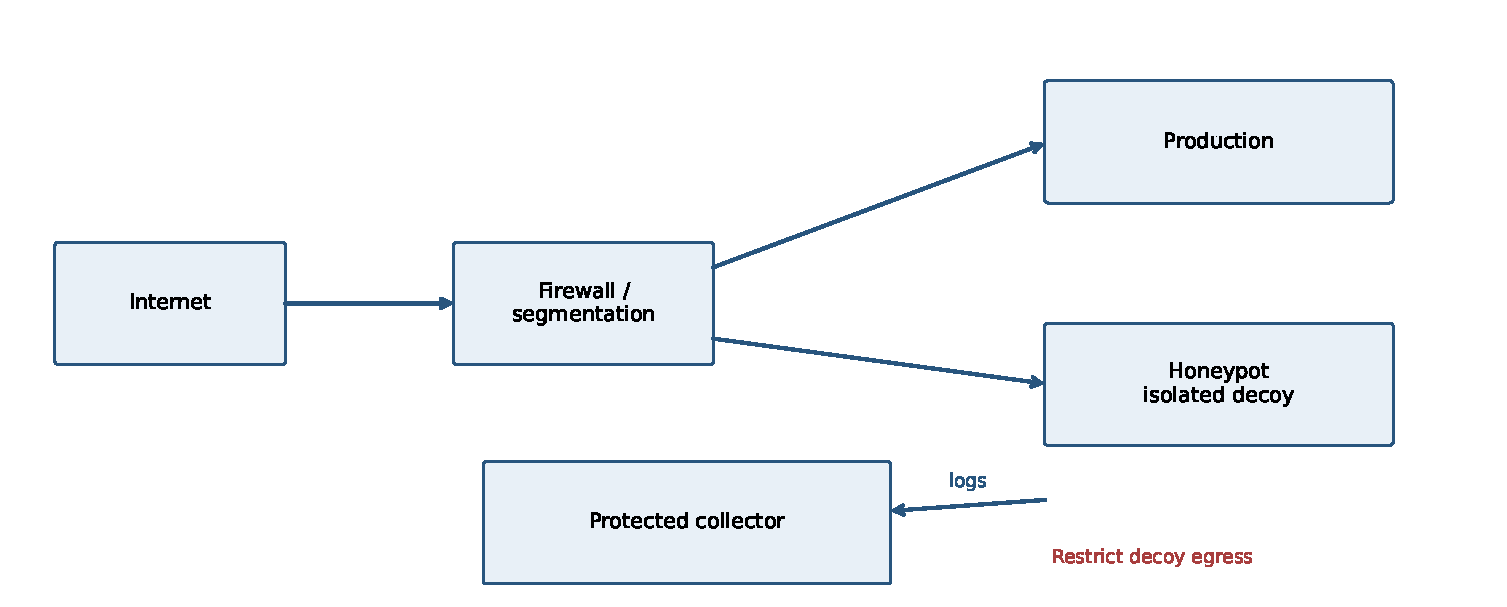
\includegraphics[width=\linewidth,height=.34\textheight,keepaspectratio]{assets/honeypot.pdf}
\end{center}



A honeypot is a deliberately attractive decoy with little or no legitimate production use. Access attempts provide comparatively high-signal evidence. Interaction can reveal exploit methods,\allowbreak{} malware,\allowbreak{} commands and C\&C destinations,\allowbreak{} and may divert an intruder from valuable systems.


Place it in a controlled segment/\allowbreak{}DMZ,\allowbreak{} monitor it from a protected collector and restrict its outbound reach. Never give it real credentials or a path for unrestricted attacks on production or third parties. A low-interaction decoy emulates selected services; a high-interaction host provides richer evidence at greater containment/\allowbreak{}maintenance cost.


\textbf{Overhead is not zero and has no fixed percentage in the question.} Costs include a VM/\allowbreak{}host,\allowbreak{} storage,\allowbreak{} logs,\allowbreak{} monitoring,\allowbreak{} analyst time,\allowbreak{} patch/\allowbreak{}reset work and some network traffic. A passive or separately segmented decoy need not sit in the production request path,\allowbreak{} so ordinary requests do not inherently incur an extra hop. Attack traffic or poor placement can nevertheless affect shared resources.


A honeypot observes attacks that touch it; it cannot replace general IDS,\allowbreak{} patching and access control.




\clearpage
\subsection{A032 · 2022–23 · Q4(c)}\label{a032}

\textbf{Stateful versus stateless filtering · 7 marks}


Original: \href{../../CSE405-Security_Merged.pdf\#page=12}{past-paper PDF p. 12}. Sitting date: 18 April 2024. Printed Section A.


\textbf{Topics:} Firewall state,\allowbreak{} evasion and defense limits.



\begin{quote}\small

\textbf{Question summary:} Compare stateful and stateless firewalls.



\end{quote}


\Needspace{4\baselineskip}
{\color{ForestGreen}\textbf{Exam tip.} Give an example packet accepted by a simplistic stateless rule but rejected for lack of state.}



{\small\setlength{\tabcolsep}{3pt}
\begin{longtable}{>{\raggedright\arraybackslash}p{0.22669\linewidth}>{\raggedright\arraybackslash}p{0.36032\linewidth}>{\raggedright\arraybackslash}p{0.37141\linewidth}}
\toprule
\textbf{Property} & \textbf{Stateless filter} & \textbf{Stateful filter} \\
\midrule
\endhead
Decision input & Current packet's fields and rules & Packet plus tracked flow/\allowbreak{}connection context \\
Return traffic & Must be allowed by explicit broad rules & Can allow replies to an established permitted flow \\
Unsolicited SYN-ACK & Could match a permissive source-port/\allowbreak{}flag rule & Can reject if no matching connection state exists \\
Resource use & Usually lower per-flow storage & State table consumes memory and can be exhausted \\
Visibility limit & Header rules do not establish application safety & Being part of a flow does not make its payload safe \\
\bottomrule
\end{longtable}
}

Stateful filtering follows TCP transitions/\allowbreak{}tuples and may validate sequence windows; exact tracking varies. UDP “state” generally means inferred tuple/\allowbreak{}time-based associations,\allowbreak{} not a UDP handshake. Application parsing and TLS decryption are additional capabilities,\allowbreak{} not guaranteed by the term stateful.




\clearpage
\subsection{A058 · 2021–22 · Q5(b)}\label{a058}

\textbf{AH versus ESP and transport/\allowbreak{}tunnel layouts · 12 marks}


Original: \href{../../CSE405-Security_Merged.pdf\#page=16}{past-paper PDF p. 16}. Sitting date: 30 October 2023. Printed Section B.


\textbf{Topics:} VPN and IPsec AH/\allowbreak{}ESP encapsulation.



\begin{quote}\small

\textbf{Question summary:} Compare IPsec AH and ESP with their encapsulations.



\end{quote}


\Needspace{4\baselineskip}
{\color{ForestGreen}\textbf{Exam tip.} Mark the exact encrypted/\allowbreak{}authenticated region instead of saying simply “AH authenticates,\allowbreak{} ESP encrypts.”}


\textbf{AH} provides packet integrity/\allowbreak{}data-origin authentication and anti-replay when enabled,\allowbreak{} but no confidentiality. Its authentication covers payload and selected immutable/\allowbreak{}predictable IP-header fields; mutable fields cannot be protected unchanged across transit.


\textbf{ESP} protects the encapsulated payload with confidentiality and,\allowbreak{} when configured,\allowbreak{} integrity/\allowbreak{}authentication (normally combined in secure deployments). It does not authenticate the outer IP header in the same way as AH. Anti-replay uses sequence numbers and a receiver window,\allowbreak{} with authenticated integrity necessary to trust them.



\begin{Verbatim}[breaklines=true,breakanywhere=true,fontsize=\small,frame=single,rulecolor=\color{PanelBorder}]
AH transport: IP | AH | TCP/UDP | data
AH tunnel:    new IP | AH | original IP | TCP/UDP | data
ESP transport: IP | ESP hdr | {TCP/UDP | data | ESP trailer} | auth tag
ESP tunnel: new IP | ESP hdr | {original IP | TCP/UDP | data | trailer} | tag
\end{Verbatim}

Braces mark the ESP-encrypted part when encryption is selected. ESP header fields such as SPI/\allowbreak{}sequence number remain visible but are integrity-protected when authentication is used. Tunnel mode hides the inner addresses from ordinary transit observation while outer endpoints remain visible.


AH's protection of address fields makes ordinary NAT problematic. ESP can traverse NAT using UDP encapsulation; do not claim all IPsec is intrinsically incompatible with NAT.



\begin{center}
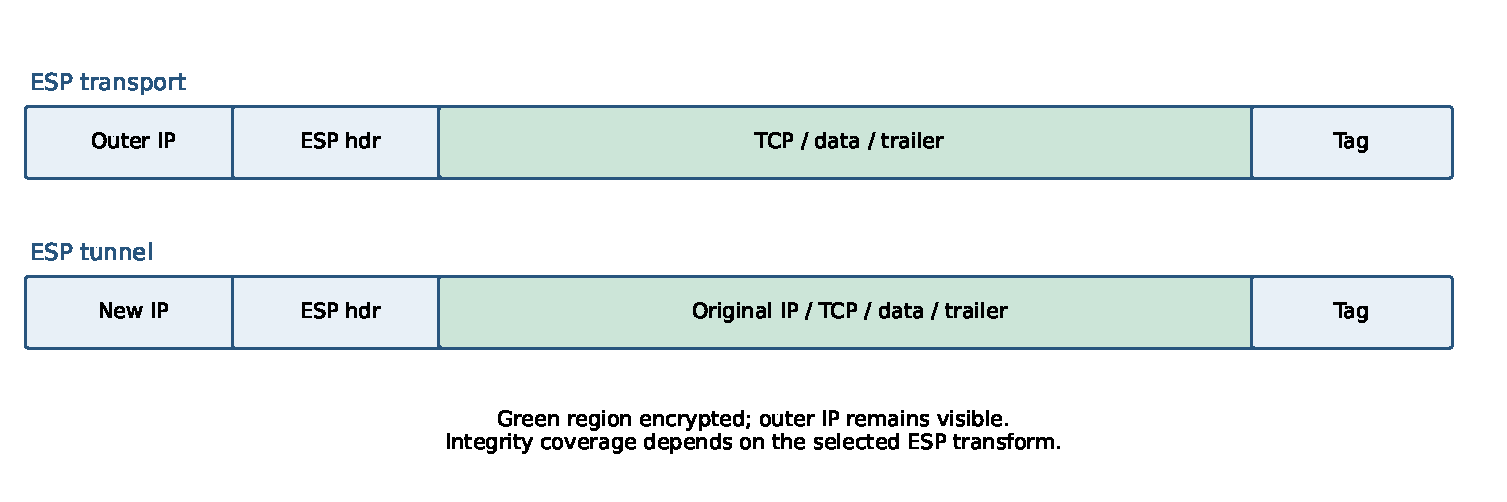
\includegraphics[width=\linewidth,height=.34\textheight,keepaspectratio]{assets/ipsec.pdf}
\end{center}



\href{https://www.rfc-editor.org/rfc/rfc4302}{References: RFC 4302},\allowbreak{} \href{https://www.rfc-editor.org/rfc/rfc4303}{RFC 4303}.




\clearpage
\subsection{A062 · 2021–22 · Q6(c)}\label{a062}

\textbf{Honeypot topology and effect on normal operation · 11 marks}


Original: \href{../../CSE405-Security_Merged.pdf\#page=17}{past-paper PDF p. 17}. Sitting date: 30 October 2023. Printed Section B.


\textbf{Topics:} Honeypot topology,\allowbreak{} monitoring and overhead.



\begin{quote}\small

\textbf{Question summary:} Explain the need for a honeypot with topology and whether it hampers normal operation.



\end{quote}


\Needspace{4\baselineskip}
{\color{ForestGreen}\textbf{Exam tip.} Distinguish direct production latency from operational and shared-resource cost.}



\begin{center}
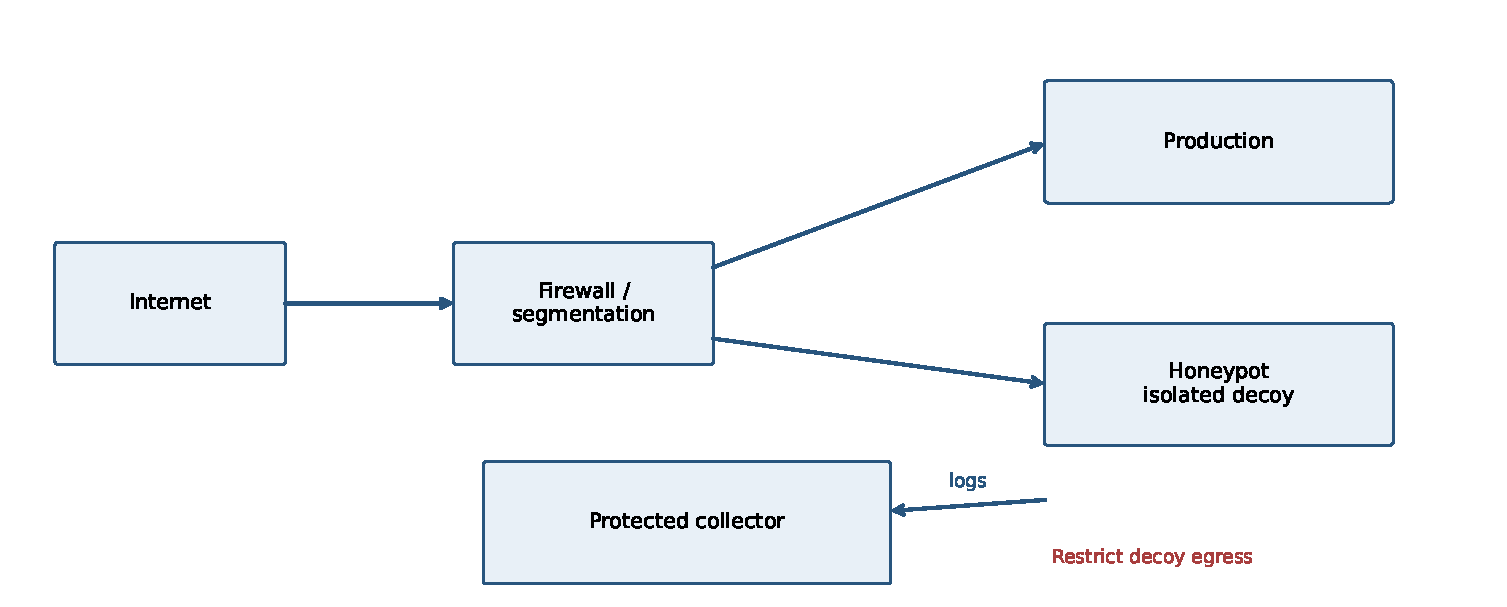
\includegraphics[width=\linewidth,height=.34\textheight,keepaspectratio]{assets/honeypot.pdf}
\end{center}



A honeypot is a deliberately attractive decoy with little or no legitimate production use. Access attempts provide comparatively high-signal evidence. Interaction can reveal exploit methods,\allowbreak{} malware,\allowbreak{} commands and C\&C destinations,\allowbreak{} and may divert an intruder from valuable systems.


Place it in a controlled segment/\allowbreak{}DMZ,\allowbreak{} monitor it from a protected collector and restrict its outbound reach. Never give it real credentials or a path for unrestricted attacks on production or third parties. A low-interaction decoy emulates selected services; a high-interaction host provides richer evidence at greater containment/\allowbreak{}maintenance cost.


\textbf{Overhead is not zero and has no fixed percentage in the question.} Costs include a VM/\allowbreak{}host,\allowbreak{} storage,\allowbreak{} logs,\allowbreak{} monitoring,\allowbreak{} analyst time,\allowbreak{} patch/\allowbreak{}reset work and some network traffic. A passive or separately segmented decoy need not sit in the production request path,\allowbreak{} so ordinary requests do not inherently incur an extra hop. Attack traffic or poor placement can nevertheless affect shared resources.


A honeypot observes attacks that touch it; it cannot replace general IDS,\allowbreak{} patching and access control.




\clearpage
\subsection{A067 · 2021–22 · Q8(b)}\label{a067}

\textbf{OS fingerprinting to validated vulnerability finding · 12 marks}


Original: \href{../../CSE405-Security_Merged.pdf\#page=17}{past-paper PDF p. 17}. Sitting date: 30 October 2023. Printed Section B.


\textbf{Topics:} Reconnaissance,\allowbreak{} fingerprinting and vulnerability assessment.



\begin{quote}\small

\textbf{Question summary:} Formulate the steps for exploiting a target after scanning its OS version.



\end{quote}


\Needspace{4\baselineskip}
{\color{ForestGreen}\textbf{Exam tip.} Separate discovery,\allowbreak{} vulnerability inference and demonstrated exploitation. Each has different evidence.}


In the exam's authorized test environment:



\begin{enumerate}

\item Define the permitted hosts/\allowbreak{}services and obtain a baseline of expected availability.

\item Discover live hosts and open ports. A TCP connect scan completes a connection; a SYN scan interprets SYN-ACK/\allowbreak{}RST without completing an ordinary connection. Filtering/\allowbreak{}timeouts require careful interpretation.

\item Identify service banners/\allowbreak{}protocol behavior and estimate OS/\allowbreak{}version using tools such as Nmap. A banner is evidence,\allowbreak{} not proof: it can be hidden,\allowbreak{} misleading or refer to a backported patched build.

\item Match the exact product,\allowbreak{} version,\allowbreak{} configuration and platform against vendor advisories/\allowbreak{}CVE records. Check authentication requirements,\allowbreak{} exposed interfaces and patch status.

\item Validate the suspected issue safely in an isolated equivalent system,\allowbreak{} then demonstrate only the agreed impact on the test target. A version match alone does not establish successful code execution.

\item Preserve evidence,\allowbreak{} explain the root cause,\allowbreak{} patch or reconfigure,\allowbreak{} reduce exposure and retest the specific finding.

\end{enumerate}

The slides mention scanners/\allowbreak{}exploit tools; a good answer connects each tool's observation to the next decision rather than treating a scan result as automatic access.




\clearpage
\subsection{A068 · 2021–22 · Q8(c)}\label{a068}

\textbf{Address-book allowlist as a spam policy · 11 marks}


Original: \href{../../CSE405-Security_Merged.pdf\#page=17}{past-paper PDF p. 17}. Sitting date: 30 October 2023. Printed Section B.


\textbf{Topics:} Firewall state,\allowbreak{} evasion and defense limits.



\begin{quote}\small

\textbf{Question summary:} Alice rejects all email except senders in her address book. Is this an effective spam defense?



\end{quote}

\textbf{Coverage:} related application/\allowbreak{}extension. Applies allowlist policy and sender-identity validation; email-specific authentication is supplementary.



\Needspace{4\baselineskip}
{\color{ForestGreen}\textbf{Exam tip.} Discuss both false negatives (spam from “allowed” identities) and false positives (new legitimate contacts).}


It reduces mail from unknown addresses but is neither complete spam prevention nor an acceptable policy for every user. An address-book entry is usually an \textbf{address string},\allowbreak{} not a cryptographic authentication of the sender. Attackers can forge visible From fields,\allowbreak{} exploit look-alike addresses or send from an actually compromised contact account.


Conversely,\allowbreak{} legitimate first-time senders,\allowbreak{} new staff,\allowbreak{} receipts and changed addresses may be rejected. That is a false-positive/\allowbreak{}usability cost and may cause users to disable the policy.


Use authenticated domain/\allowbreak{}message evidence,\allowbreak{} reputation/\allowbreak{}content controls and a quarantine/\allowbreak{}review path appropriate to the user's needs. SPF/\allowbreak{}DKIM/\allowbreak{}DMARC provide useful domain-level signals but do not prove a contact's account is uncompromised or every message benign. Strong allowlisting should use the intended authenticated identity rather than trusting a display name.




\clearpage
\subsection{A076 · 2020–21 · Q3(b)}\label{a076}

\textbf{Web-server assessment and validation workflow · 12 marks}


Original: \href{../../CSE405-Security_Merged.pdf\#page=18}{past-paper PDF p. 18}. Sitting date: 25 September 2022. Printed Section A.


\textbf{Topics:} Reconnaissance,\allowbreak{} fingerprinting and vulnerability assessment.



\begin{quote}\small

\textbf{Question summary:} Give a stepwise approach and tools to find and exploit popular web-server vulnerabilities.



\end{quote}


\Needspace{4\baselineskip}
{\color{ForestGreen}\textbf{Exam tip.} Separate discovery,\allowbreak{} vulnerability inference and demonstrated exploitation. Each has different evidence.}


In the exam's authorized test environment:



\begin{enumerate}

\item Define the permitted hosts/\allowbreak{}services and obtain a baseline of expected availability.

\item Discover live hosts and open ports. A TCP connect scan completes a connection; a SYN scan interprets SYN-ACK/\allowbreak{}RST without completing an ordinary connection. Filtering/\allowbreak{}timeouts require careful interpretation.

\item Identify service banners/\allowbreak{}protocol behavior and estimate OS/\allowbreak{}version using tools such as Nmap. A banner is evidence,\allowbreak{} not proof: it can be hidden,\allowbreak{} misleading or refer to a backported patched build.

\item Match the exact product,\allowbreak{} version,\allowbreak{} configuration and platform against vendor advisories/\allowbreak{}CVE records. Check authentication requirements,\allowbreak{} exposed interfaces and patch status.

\item Validate the suspected issue safely in an isolated equivalent system,\allowbreak{} then demonstrate only the agreed impact on the test target. A version match alone does not establish successful code execution.

\item Preserve evidence,\allowbreak{} explain the root cause,\allowbreak{} patch or reconfigure,\allowbreak{} reduce exposure and retest the specific finding.

\end{enumerate}

The slides mention scanners/\allowbreak{}exploit tools; a good answer connects each tool's observation to the next decision rather than treating a scan result as automatic access.


For a web server,\allowbreak{} also inventory enabled modules,\allowbreak{} TLS termination,\allowbreak{} reverse proxies and application versions; the externally visible Server header may not identify the vulnerable component. Validate the exact HTTP path/\allowbreak{}feature involved and use a reproducible minimal test with agreed limits.




\clearpage
\subsection{A080 · 2020–21 · Q4(c)}\label{a080}

\textbf{Base-rate fallacy with a numerical example · 11 marks}


Original: \href{../../CSE405-Security_Merged.pdf\#page=19}{past-paper PDF p. 19}. Sitting date: 25 September 2022. Printed Section A.


\textbf{Topics:} Intrusion detection,\allowbreak{} base rates and audit data.



\begin{quote}\small

\textbf{Question summary:} Define the base-rate fallacy,\allowbreak{} give an example and explain its effect on daily incident handling.



\end{quote}

\textbf{Coverage:} related application/\allowbreak{}extension. The deck teaches the four alarm outcomes; Bayes/\allowbreak{}base-rate calculation is an extension.



\Needspace{4\baselineskip}
{\color{ForestGreen}\textbf{Exam tip.} Use a confusion matrix or natural event counts,\allowbreak{} then compute true alarms divided by all alarms.}


The fallacy is treating a detector's high sensitivity or low false-positive rate as the probability that an \textbf{alarm} is a real attack,\allowbreak{} while ignoring how rare attacks are.


Let attack prevalence \(p=0.001\),\allowbreak{} sensitivity \(s=0.99\) and false-positive rate \(f=0.01\). Bayes' rule gives



\[
P(A\mid +)=\frac{sp}{sp+f(1-p)}=\frac{0.00099}{0.00099+0.00999}\approx 0.0902.
\]

Among 100,\allowbreak{}000 events,\allowbreak{} expect 100 attacks,\allowbreak{} 99 true alarms,\allowbreak{} 99,\allowbreak{}900 benign events and 999 false alarms. Only about \textbf{9\% of alarms} are true despite 99\% sensitivity and 99\% specificity.


Analysts face alert fatigue,\allowbreak{} wasted effort and delayed responses to real incidents. Improve precision through context/\allowbreak{}correlation,\allowbreak{} sensible thresholds,\allowbreak{} validated high-value rules and triage; reducing false positives must be balanced against false negatives. Track prevalence and evaluate precision as well as recall.




\clearpage
\subsection{A094 · 2019–20 · Q2(c)}\label{a094}

\textbf{Verify a reported DoS source and respond with evidence · 11 marks}


Original: \href{../../CSE405-Security_Merged.pdf\#page=22}{past-paper PDF p. 22}. Sitting date: 07 September 2021. Printed Section A.


\textbf{Topics:} Intrusion detection,\allowbreak{} base rates and audit data; OS trust,\allowbreak{} paging,\allowbreak{} boot and persistent memory images; DoS/\allowbreak{}DDoS,\allowbreak{} reflection and resource exhaustion.



\begin{quote}\small

\textbf{Question summary:} A hall administrator says your shared network segment is sending DoS traffic. You deny involvement but are unsure about your roommate. How do you verify and respond?



\end{quote}

\textbf{Coverage:} related application/\allowbreak{}extension. Uses IDS/\allowbreak{}network logs and OS event logging; incident-handling workflow extends the slides.



\Needspace{4\baselineskip}
{\color{ForestGreen}\textbf{Exam tip.} Explain attribution limits and the sequence verify → contain → investigate → recover.}


Ask for concrete indicators: timestamps/\allowbreak{}time zone,\allowbreak{} observed source IP/\allowbreak{}port,\allowbreak{} destination,\allowbreak{} protocol,\allowbreak{} traffic rate and available logs. Confirm the report through an independent known contact path rather than trusting an unsolicited caller.


Correlate those observations with local process/\allowbreak{}network logs,\allowbreak{} router/\allowbreak{}DHCP/\allowbreak{}NAT mappings and switch ingress records. A shared public IP or segment does not uniquely identify a roommate; source IPs can also be spoofed. Capture only the relevant authorized traffic and inspect for sustained abnormal outgoing connections,\allowbreak{} malware or unexpected processes.


If evidence suggests an affected machine,\allowbreak{} coordinate containment with the administrator: isolate the specific host/\allowbreak{}port,\allowbreak{} preserve useful evidence,\allowbreak{} remove/\allowbreak{}rebuild the compromised environment,\allowbreak{} patch the entry point and rotate exposed credentials. Block abusive traffic while allowing essential investigation,\allowbreak{} then verify that it has stopped. Do not accuse an individual solely from a shared address or erase all logs before diagnosis.




\clearpage
\subsection{A101 · 2019–20 · Q5(a)}\label{a101}

\textbf{PIDS,\allowbreak{} alarm outcomes and base-rate interpretation · 14 marks}


Original: \href{../../CSE405-Security_Merged.pdf\#page=24}{past-paper PDF p. 24}. Sitting date: 07 September 2021. Printed Section B.


\textbf{Topics:} Intrusion detection,\allowbreak{} base rates and audit data.



\begin{quote}\small

\textbf{Question summary:} Define protocol-based IDS,\allowbreak{} list alarm outcomes and explain base-rate fallacy.



\end{quote}

\textbf{Coverage:} related application/\allowbreak{}extension. IDS and the confusion matrix are explicit; PIDS specialization and Bayesian analysis are supplementary.



\Needspace{4\baselineskip}
{\color{ForestGreen}\textbf{Exam tip.} Use a confusion matrix or natural event counts,\allowbreak{} then compute true alarms divided by all alarms.}


A \textbf{protocol-based IDS (PIDS)} observes a protocol's messages,\allowbreak{} state transitions and expected semantics at a host/\allowbreak{}service or network boundary. It can detect invalid sequences or known malicious protocol patterns; mere TCP connectivity is not evidence that the application exchange is valid.



{\small\setlength{\tabcolsep}{3pt}
\begin{longtable}{>{\raggedright\arraybackslash}p{0.30327\linewidth}>{\raggedright\arraybackslash}p{0.32757\linewidth}>{\raggedright\arraybackslash}p{0.32757\linewidth}}
\toprule
\textbf{Actual event} & \textbf{Alarm} & \textbf{No alarm} \\
\midrule
\endhead
Attack & True positive & False negative \\
Benign & False positive & True negative \\
\bottomrule
\end{longtable}
}

The fallacy is treating a detector's high sensitivity or low false-positive rate as the probability that an \textbf{alarm} is a real attack,\allowbreak{} while ignoring how rare attacks are.


Let attack prevalence \(p=0.001\),\allowbreak{} sensitivity \(s=0.99\) and false-positive rate \(f=0.01\). Bayes' rule gives



\[
P(A\mid +)=\frac{sp}{sp+f(1-p)}=\frac{0.00099}{0.00099+0.00999}\approx 0.0902.
\]

Among 100,\allowbreak{}000 events,\allowbreak{} expect 100 attacks,\allowbreak{} 99 true alarms,\allowbreak{} 99,\allowbreak{}900 benign events and 999 false alarms. Only about \textbf{9\% of alarms} are true despite 99\% sensitivity and 99\% specificity.


Analysts face alert fatigue,\allowbreak{} wasted effort and delayed responses to real incidents. Improve precision through context/\allowbreak{}correlation,\allowbreak{} sensible thresholds,\allowbreak{} validated high-value rules and triage; reducing false positives must be balanced against false negatives. Track prevalence and evaluate precision as well as recall.




\clearpage
\subsection{A102 · 2019–20 · Q5(b)}\label{a102}

\textbf{Audit-record fields and statistical intrusion detection · 14 marks}


Original: \href{../../CSE405-Security_Merged.pdf\#page=24}{past-paper PDF p. 24}. Sitting date: 07 September 2021. Printed Section B.


\textbf{Topics:} Intrusion detection,\allowbreak{} base rates and audit data; OS trust,\allowbreak{} paging,\allowbreak{} boot and persistent memory images.



\begin{quote}\small

\textbf{Question summary:} List useful audit-record fields,\allowbreak{} explain statistical IDS and identify a weakness.



\end{quote}

\textbf{Coverage:} related application/\allowbreak{}extension. Event logging and IDS sensors are taught; statistical-model design is an extension.



\Needspace{4\baselineskip}
{\color{ForestGreen}\textbf{Exam tip.} Tie the listed audit fields to the behaviors your model actually measures.}


A useful event record includes timestamp/\allowbreak{}time zone,\allowbreak{} event/\allowbreak{}record ID,\allowbreak{} host/\allowbreak{}sensor,\allowbreak{} authenticated user/\allowbreak{}process and effective identity,\allowbreak{} action,\allowbreak{} target object/\allowbreak{}resource,\allowbreak{} source/\allowbreak{}destination addresses/\allowbreak{}ports as appropriate,\allowbreak{} outcome/\allowbreak{}error code and a correlation/\allowbreak{}session ID. Include enough context to link events without needlessly recording passwords or sensitive payloads.


A statistical/\allowbreak{}anomaly IDS builds a baseline or model of normal activity—such as login frequency,\allowbreak{} transfer volume,\allowbreak{} process behavior or service access. It scores new observations against that model and alerts on a threshold deviation or unlikely combination. Training,\allowbreak{} feature choice,\allowbreak{} aggregation window and threshold determine behavior.


A principal weakness is that \textbf{unusual is not identical to malicious}: legitimate new work can cause false alarms,\allowbreak{} while an attacker mimicking normal behavior may evade detection. Concept drift,\allowbreak{} compromised training data and low attack prevalence further complicate performance. Validate with labeled evidence and context,\allowbreak{} and combine anomaly scores with other signals.




\clearpage
\subsection{A103 · 2019–20 · Q5(c)}\label{a103}

\textbf{Why a decoy helps intrusion detection · 7 marks}


Original: \href{../../CSE405-Security_Merged.pdf\#page=24}{past-paper PDF p. 24}. Sitting date: 07 September 2021. Printed Section B.


\textbf{Topics:} Honeypot topology,\allowbreak{} monitoring and overhead.



\begin{quote}\small

\textbf{Question summary:} Explain why a honeypot is an effective IDS tool.



\end{quote}


\Needspace{4\baselineskip}
{\color{ForestGreen}\textbf{Exam tip.} Distinguish direct production latency from operational and shared-resource cost.}



\begin{center}
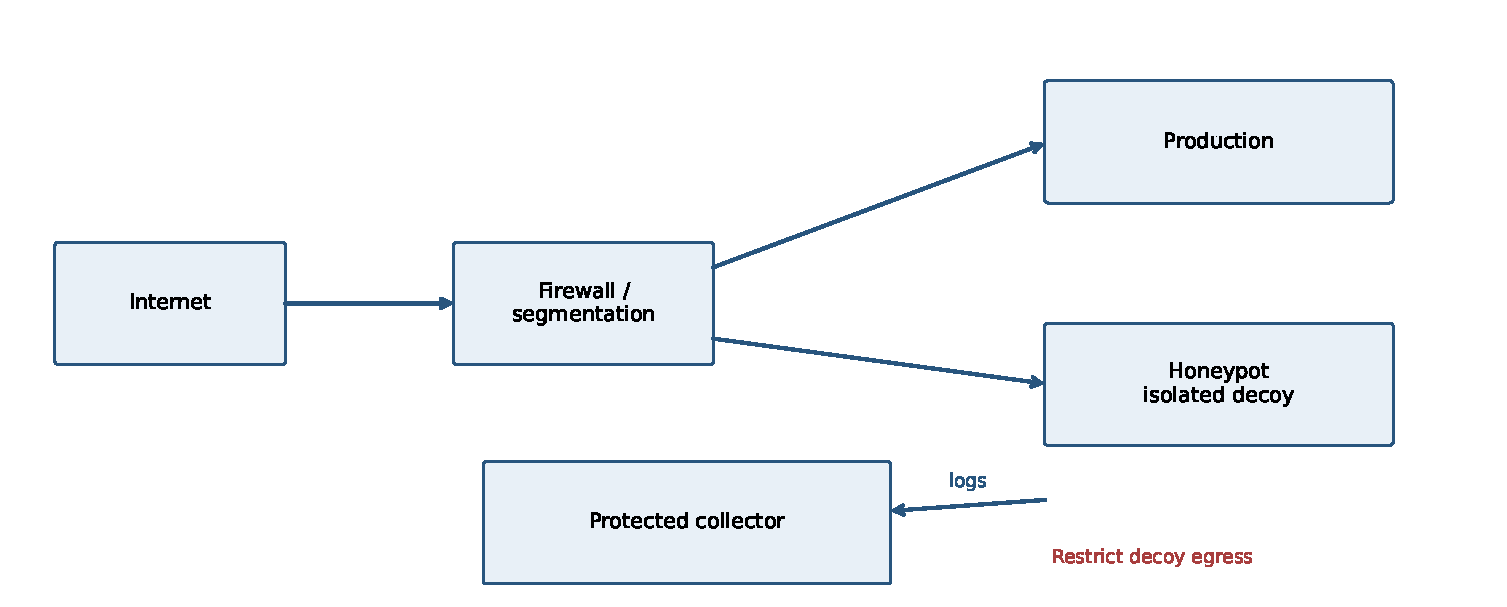
\includegraphics[width=\linewidth,height=.34\textheight,keepaspectratio]{assets/honeypot.pdf}
\end{center}



A honeypot is a deliberately attractive decoy with little or no legitimate production use. Access attempts provide comparatively high-signal evidence. Interaction can reveal exploit methods,\allowbreak{} malware,\allowbreak{} commands and C\&C destinations,\allowbreak{} and may divert an intruder from valuable systems.


Place it in a controlled segment/\allowbreak{}DMZ,\allowbreak{} monitor it from a protected collector and restrict its outbound reach. Never give it real credentials or a path for unrestricted attacks on production or third parties. A low-interaction decoy emulates selected services; a high-interaction host provides richer evidence at greater containment/\allowbreak{}maintenance cost.


\textbf{Overhead is not zero and has no fixed percentage in the question.} Costs include a VM/\allowbreak{}host,\allowbreak{} storage,\allowbreak{} logs,\allowbreak{} monitoring,\allowbreak{} analyst time,\allowbreak{} patch/\allowbreak{}reset work and some network traffic. A passive or separately segmented decoy need not sit in the production request path,\allowbreak{} so ordinary requests do not inherently incur an extra hop. Attack traffic or poor placement can nevertheless affect shared resources.


A honeypot observes attacks that touch it; it cannot replace general IDS,\allowbreak{} patching and access control.




\clearpage
\subsection{A111 · 2018–19 · Q1(b)}\label{a111}

\textbf{Compare IPsec ESP and AH formats · 9 marks}


Original: \href{../../CSE405-Security_Merged.pdf\#page=26}{past-paper PDF p. 26}. Sitting date: 24 October 2019. Printed Section A.


\textbf{Topics:} VPN and IPsec AH/\allowbreak{}ESP encapsulation.



\begin{quote}\small

\textbf{Question summary:} Contrast IPsec AH and ESP,\allowbreak{} including header encapsulations.



\end{quote}


\Needspace{4\baselineskip}
{\color{ForestGreen}\textbf{Exam tip.} Mark the exact encrypted/\allowbreak{}authenticated region instead of saying simply “AH authenticates,\allowbreak{} ESP encrypts.”}


\textbf{AH} provides packet integrity/\allowbreak{}data-origin authentication and anti-replay when enabled,\allowbreak{} but no confidentiality. Its authentication covers payload and selected immutable/\allowbreak{}predictable IP-header fields; mutable fields cannot be protected unchanged across transit.


\textbf{ESP} protects the encapsulated payload with confidentiality and,\allowbreak{} when configured,\allowbreak{} integrity/\allowbreak{}authentication (normally combined in secure deployments). It does not authenticate the outer IP header in the same way as AH. Anti-replay uses sequence numbers and a receiver window,\allowbreak{} with authenticated integrity necessary to trust them.



\begin{Verbatim}[breaklines=true,breakanywhere=true,fontsize=\small,frame=single,rulecolor=\color{PanelBorder}]
AH transport: IP | AH | TCP/UDP | data
AH tunnel:    new IP | AH | original IP | TCP/UDP | data
ESP transport: IP | ESP hdr | {TCP/UDP | data | ESP trailer} | auth tag
ESP tunnel: new IP | ESP hdr | {original IP | TCP/UDP | data | trailer} | tag
\end{Verbatim}

Braces mark the ESP-encrypted part when encryption is selected. ESP header fields such as SPI/\allowbreak{}sequence number remain visible but are integrity-protected when authentication is used. Tunnel mode hides the inner addresses from ordinary transit observation while outer endpoints remain visible.


AH's protection of address fields makes ordinary NAT problematic. ESP can traverse NAT using UDP encapsulation; do not claim all IPsec is intrinsically incompatible with NAT.



\begin{center}
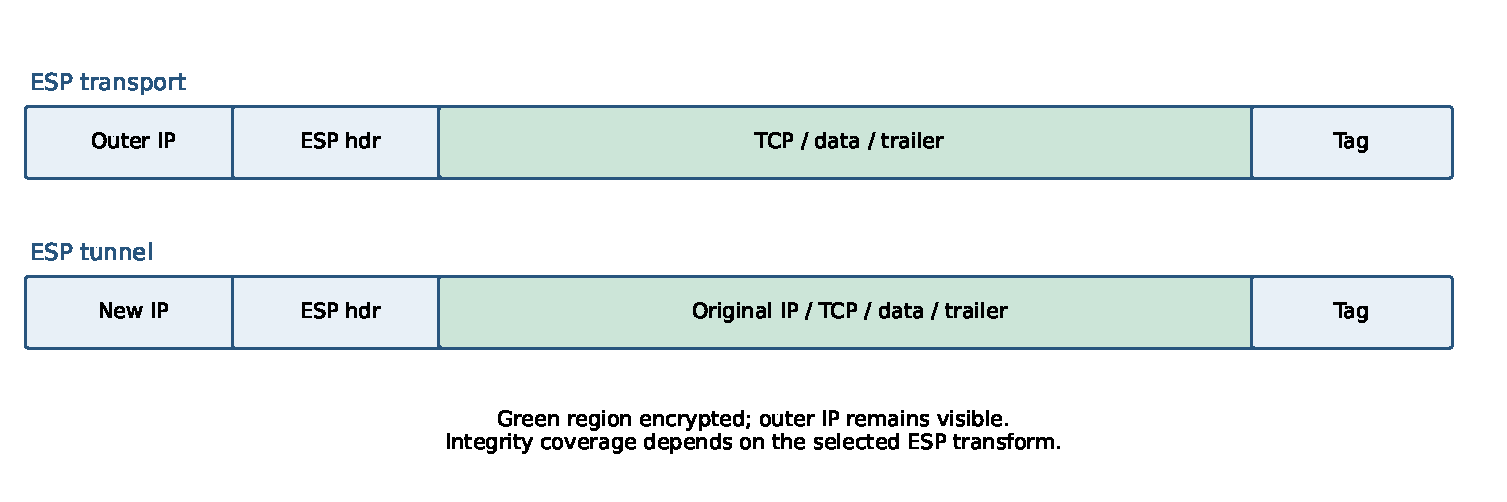
\includegraphics[width=\linewidth,height=.34\textheight,keepaspectratio]{assets/ipsec.pdf}
\end{center}



\href{https://www.rfc-editor.org/rfc/rfc4302}{References: RFC 4302},\allowbreak{} \href{https://www.rfc-editor.org/rfc/rfc4303}{RFC 4303}.




\clearpage
\subsection{A124 · 2018–19 · Q4(c)}\label{a124}

\textbf{Rule-based ARP-spoofing detection · 9 marks}


Original: \href{../../CSE405-Security_Merged.pdf\#page=26}{past-paper PDF p. 26}. Sitting date: 24 October 2019. Printed Section A.


\textbf{Topics:} Intrusion detection,\allowbreak{} base rates and audit data; ARP spoofing,\allowbreak{} MITM and detection.



\begin{quote}\small

\textbf{Question summary:} Give rules a rule-based IDS can use to detect ARP spoofing.



\end{quote}


\Needspace{4\baselineskip}
{\color{ForestGreen}\textbf{Exam tip.} Make the rule testable—state fields,\allowbreak{} trusted expectation and alert condition.}


Useful rules compare observations with trusted bindings and expected behavior:



\begin{itemize}

\item Alert when a protected IP,\allowbreak{} especially the gateway,\allowbreak{} is claimed by an unexpected MAC.

\item Alert on rapid IP-to-MAC binding changes or conflicting replies for one IP.

\item Flag ARP replies inconsistent with trusted DHCP-snooping/\allowbreak{}static bindings or arriving from an unauthorized ingress port.

\item Investigate excessive unsolicited/\allowbreak{}gratuitous ARP or one unexpected MAC claiming many unrelated hosts.

\end{itemize}

Correlate packet data with switch-port identity,\allowbreak{} lease records and known maintenance/\allowbreak{}failover events. A gratuitous reply or shared MAC is not automatically malicious: virtual routers,\allowbreak{} failover and proxy ARP can be legitimate. Rules need baselines/\allowbreak{}exceptions and must be evaluated for false positives/\allowbreak{}negatives.


An IDS typically alerts; DAI on a switch can enforce bindings and drop invalid packets. The same evidence can inform both,\allowbreak{} but detection and prevention are different actions.




\clearpage
\subsection{A125 · 2018–19 · Q4(d)}\label{a125}

\textbf{Honeypot detection,\allowbreak{} evidence and diversion · 8 marks}


Original: \href{../../CSE405-Security_Merged.pdf\#page=26}{past-paper PDF p. 26}. Sitting date: 24 October 2019. Printed Section A.


\textbf{Topics:} Honeypot topology,\allowbreak{} monitoring and overhead.



\begin{quote}\small

\textbf{Question summary:} Explain honeypot use cases with a diagram.



\end{quote}


\Needspace{4\baselineskip}
{\color{ForestGreen}\textbf{Exam tip.} Distinguish direct production latency from operational and shared-resource cost.}



\begin{center}
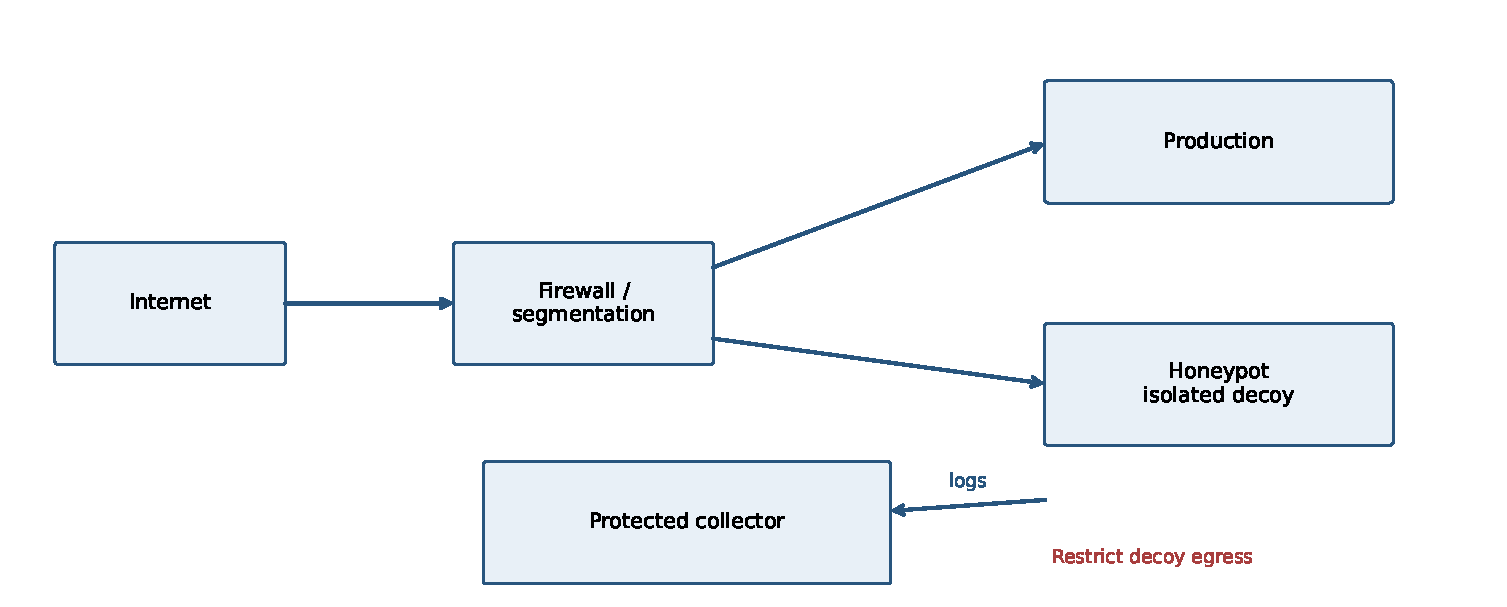
\includegraphics[width=\linewidth,height=.34\textheight,keepaspectratio]{assets/honeypot.pdf}
\end{center}



A honeypot is a deliberately attractive decoy with little or no legitimate production use. Access attempts provide comparatively high-signal evidence. Interaction can reveal exploit methods,\allowbreak{} malware,\allowbreak{} commands and C\&C destinations,\allowbreak{} and may divert an intruder from valuable systems.


Place it in a controlled segment/\allowbreak{}DMZ,\allowbreak{} monitor it from a protected collector and restrict its outbound reach. Never give it real credentials or a path for unrestricted attacks on production or third parties. A low-interaction decoy emulates selected services; a high-interaction host provides richer evidence at greater containment/\allowbreak{}maintenance cost.


\textbf{Overhead is not zero and has no fixed percentage in the question.} Costs include a VM/\allowbreak{}host,\allowbreak{} storage,\allowbreak{} logs,\allowbreak{} monitoring,\allowbreak{} analyst time,\allowbreak{} patch/\allowbreak{}reset work and some network traffic. A passive or separately segmented decoy need not sit in the production request path,\allowbreak{} so ordinary requests do not inherently incur an extra hop. Attack traffic or poor placement can nevertheless affect shared resources.


A honeypot observes attacks that touch it; it cannot replace general IDS,\allowbreak{} patching and access control.



\clearpage
\section{Review checklist}


\begin{itemize}

\item Protocol answers: label peers,\allowbreak{} message fields,\allowbreak{} authenticated identities,\allowbreak{} replay state and attacker position.

\item Probability answers: define the population/\allowbreak{}conditioning,\allowbreak{} compute intermediate counts and check units.

\item Memory answers: trace actual destination bounds,\allowbreak{} endianness,\allowbreak{} frame offsets and input restrictions; distinguish a control transfer from clean continuation.

\item Permission answers: distinguish real/\allowbreak{}effective identity,\allowbreak{} pathname/\allowbreak{}object identity and revocation of delegated rights.

\item Detection answers: discuss false positives,\allowbreak{} false negatives,\allowbreak{} attacker visibility and what the mechanism cannot observe.

\end{itemize}


\clearpage
\section{Sources and section scope}

Local source page maps and exam-frequency evidence are in \href{../analysis/FINAL_EXAM_TOPIC_ANALYSIS.md}{the Sec A analysis}. The \href{../analysis/SYLLABUS.md}{Sec A syllabus} defines the current topic boundary. This guide uses local Sec A answer sources and figures; it does not import Sec B answers. Older printed section labels are recorded only to locate questions,\allowbreak{} and never determine which current study guide owns a topic. Existing identifiers are preserved,\allowbreak{} so removed entries leave gaps in their numbering.


Primary technical references appear beside the answers that use them; these supplement the supplied course material rather than define a new course syllabus.


\end{document}
